\documentclass{ucetd}

% \usepackage{subfigure,epsfig,amsfonts}
% \usepackage{amsthm}
% \usepackage{natbib}
% \bibliographystyle{plain}

% \usepackage[normalem]{ulem}
% \usepackage{float}
\usepackage{url}
% \usepackage{makeidx}
% \usepackage{graphicx}
% \usepackage{graphics}
% \usepackage{multicol}
% \usepackage{xspace}
% \usepackage{chngpage}
%\usepackage{narrow}
%\usepackage{fullpage}
%\usepackage{subfigure}
\usepackage{subfig}
\usepackage{multirow}
\usepackage{rotating}
\usepackage{xcolor}
%\usepackage{algorithmic2e}
\usepackage{algpseudocode}
\usepackage{algorithm}
% \usepackage{savesym}
\usepackage{amsmath}
% \usepackage{amssymb,latexsym}
% \everymath{\displaystyle}
% \savesymbol{iint} 
% \usepackage{txfonts} 
% \restoresymbol{TXF}{iint}
%\usepackage{mathptmx} % amsmath makes the paper longer
% \usepackage{mathrsfs}
%\usepackage{algorithmic}
%\usepackage{algorithm}
%\usepackage{fullpage}
%\usepackage[font={small,bf},nooneline]{caption}
% \usepackage{hyphenat}
% \usepackage{leading}
% \let\labelindent\relax
\usepackage{enumitem}
\usepackage[natbib=true,backend=bibtex,style=numeric-comp,sorting=nyt,defernumbers,maxnames=99,doi=false,isbn=false,url=false]{biblatex}
% \usepackage{balance}
% \usepackage{pbox}

\definecolor{mygreen}{rgb}{0,0.6,0}
\definecolor{mygray}{rgb}{0.5,0.5,0.5}
\definecolor{mymauve}{rgb}{0.58,0,0.82}
\usepackage{listings}
\lstset{ %
  backgroundcolor=\color{white},   % choose the background color; you must add \usepackage{color} or \usepackage{xcolor}
  basicstyle=\scriptsize\ttfamily, % the size of the fonts that are used for the code
  breakatwhitespace=false,         % sets if automatic breaks should only happen at whitespace
  breaklines=true,                 % sets automatic line breaking
  captionpos=b,                    % sets the caption-position to bottom
  commentstyle=\color{mygreen},    % comment style
  deletekeywords={...},            % if you want to delete keywords from the given language
  escapeinside={\%*}{*)},          % if you want to add LaTeX within your code
  extendedchars=true,              % lets you use non-ASCII characters; for 8-bits encodings only, does not work with UTF-8
  frame=leftline,                  % adds a frame around the code
  keepspaces=true,                 % keeps spaces in text, useful for keeping indentation of code (possibly needs columns=flexible)
  keywordstyle=\color{blue},       % keyword style
  morekeywords={*,...},            % if you want to add more keywords to the set
  numbers=left,                    % where to put the line-numbers; possible values are (none, left, right)
  numbersep=5pt,                   % how far the line-numbers are from the code
  numberstyle=\tiny\color{mygray}, % the style that is used for the line-numbers
  rulecolor=\color{black},         % if not set, the frame-color may be changed on line-breaks within not-black text (e.g. comments (green here))
  showspaces=false,                % show spaces everywhere adding particular underscores; it overrides 'showstringspaces'
  showstringspaces=false,          % underline spaces within strings only
  showtabs=false,                  % show tabs within strings adding particular underscores
  stepnumber=1,                    % the step between two line-numbers. If it's 1, each line will be numbered
  stringstyle=\color{black},     % string literal style
  tabsize=1,                       % sets default tabsize to 2 spaces
  title=\lstname                   % show the filename of files included with \lstinputlisting; also try caption instead of title
}

\usepackage{pgfplots}
% options for pgfplots
\pgfplotsset{compat=1.8,compat/show suggested version=false}
\usetikzlibrary{calc,trees,arrows,patterns,plotmarks,shapes,snakes,er,3d,automata,backgrounds,topaths,decorations.pathmorphing,decorations.markings}
%\pgfplotsset{compat=newest}
\pgfplotsset{
   /pgfplots/bar  cycle  list/.style={/pgfplots/cycle  list={%
        {black,fill=black!30!white,mark=none},%
        {black,fill=red!30!white,mark=none},%
        {black,fill=green!30!white,mark=none},%
        {black,fill=yellow!30!white,mark=none},%
        {black,fill=brown!30!white,mark=none},%
     }
   },
}
% begin of externalization
\usetikzlibrary{external}
\tikzexternalize[prefix=out/]
\tikzexternalize
% don't externalize todonotes
%\makeatletter
%\renewcommand{\todo}[2][]{\tikzexternaldisable\@todo[#1]{#2}\tikzexternalenable}
%\makeatother
% end of externalization
\usetikzlibrary{patterns}
\usepgfplotslibrary{groupplots}
\pgfplotsset{
every axis label/.append style={font=\footnotesize},
tick label style={font=\footnotesize},
}
%\usepackage[normalem]{ulem}
%\setlength{\abovecaptionskip}{2pt plus 2pt minus 2pt}
\setlist{noitemsep,topsep=0pt}

% some useful shortcuts
\newcommand{\ie}{\textit{i.e., }}
\newcommand{\eg}{\textit{e.g., }}
\newcommand{\etal}{et al.\ }
% units for results
\newcommand{\uj}{\,$\mu$J}
\newcommand{\mw}{\,mW}
\newcommand{\uw}{\,$\mu$W}
\newcommand{\ns}{\,ns}
\newcommand{\us}{\,$\mu$s}
\newcommand{\ms}{\,ms}
\newcommand{\KB}{\,KB}
\newcommand{\MB}{\,MB}
\newcommand{\GB}{\,GB}
\newcommand{\MHz}{\,MHz}
\newcommand{\GHz}{\,GHz}

\newcommand{\TODO}[1]{\textcolor{gray}{\textbf{\ [TODO:\ #1]\ }}}

% Referencing various pieces of the document:
\newcommand{\figref}[1]{Figure~\ref{fig:#1}}
\newcommand{\figsref}[2]{Figures~\ref{fig:#1} and~\ref{fig:#2}}
\newcommand{\figrref}[2]{Figures~\ref{fig:#1}--\ref{fig:#2}}
\newcommand{\secref}[1]{Chapter~\ref{sec:#1}}
\newcommand{\secsref}[2]{Sections~\ref{sec:#1} and~\ref{sec:#2}}
\newcommand{\eqnref}[1]{Eqn.~\ref{eqn:#1}}
\newcommand{\eqnsref}[2]{Eqns.~\ref{eqn:#1} and~\ref{eqn:#2}}
\newcommand{\eqnrref}[2]{Eqns.~\ref{eqn:#1}--\ref{eqn:#2}}
\newcommand{\lstref}[1]{Listing~\ref{lst:#1}}
\newcommand{\insref}[1]{Instruction~\ref{ins:#1}}
\newcommand{\tblref}[1]{Table~\ref{tbl:#1}}
\newcommand{\appref}[1]{Appendix~\ref{app:#1}}
\newcommand{\appsref}[2]{Appendices~\ref{app:#1} and~\ref{app:#2}}
\newcommand{\algoref}[1]{Algorithm~\ref{algo:#1}}

\newcommand{\argmin}{\arg\!\min}
\newcommand{\argmax}{\arg\!\max}
\newcommand{\minimize}{minimize}
\newcommand{\maximize}{maximize}
\newcommand{\optimize}{optimize}
\newcommand{\st}{s.t.}

\newcommand{\app}[1]{\mbox{\texttt{#1}}}
\newcommand{\interface}[1]{\mbox{\texttt{#1}}}
\newcommand{\function}[1]{\mbox{\texttt{#1}}}
\newcommand{\struct}[1]{\mbox{\texttt{#1}}}
\newcommand{\variable}[1]{\mbox{\texttt{#1}}}
\newcommand{\pc}[1]{\mbox{\texttt{#1}}}

% Custom hyphenation rules
\hyphenation{Ang-strom}


%% Use these commands to set biographic information for the title page:
\title{Balancing Performance and Energy in Computing Systems}
\author{Connor Kelly Imes}
\department{Computer Science}
\division{Physical Sciences}
\degree{Doctor of Philosophy}
\date{June 2018}

%% Use these commands to set a dedication and epigraph text
\dedication{\TODO{Dedication Text}}
\epigraph{\TODO{Epigraph Text}}

\bibliography{seec}


\begin{document}
%% Basic setup commands
% If you don't want a title page comment out the next line and uncomment the line after it:
\maketitle
%\omittitle

% These lines can be commented out to disable the copyright/dedication/epigraph pages
\makecopyright
% \makededication
% \makeepigraph


%% Make the various tables of contents
\tableofcontents
\listoffigures
\listoftables

\acknowledgments
% Enter Acknowledgements here
There are so many people to thank, I cannot hope to list them all here.

None of my efforts before or during graduate school would have been possible without unwavering support from my family.
In then ten years and five different states since college, time and distance have only heightened my appreciation for everything you have given me.
Thank you.
% Thanks also for an ample supply of fish.

Those who aided my journey getting here, especially...
Professor Michael Crowley at the University of Southern California, for his letter of recommendation five years after I graduated.
My coworkers from Lockheed Martin, especially Gerald Nostrand for his letter of recommendation, and for just being an awesome technical manager---thanks for letting us be engineers.

Professor Hank Hoffmann, the best advisor a graduate student could ask for...
Besides the exceptional mentoring and support which would require a whole other document to describe, thanks for off-topic conversations, and for taking me into your confidence far more than most advisors ever would.
And for sending me \emph{everywhere}, especially Portugal, Hong Kong, Greece, and France.
I wish you could have joined in the adventures, but thanks also for trusting me to ``spread the gospel'' and defend our work on my own.
Now that you have tenure, my work here is done!

Also at the University of Chicago, especially...
Professors Andrew Chien and Haryadi Gunawi, for being on my Master's committee.
Professor Shan Lu, for being on my doctoral dissertation committee.
Nikita Mishra and David Kim, for collaborations and co-authorships.
Huazhe (Harper) Zhang and Kevin Zhao, for helping with the grunt work.
Ivana Marin{\u c}i{\'c}, for being well-connected and helping my with my job hunt.
The department technical and administrative staff, especially Bob Bartlett, Margaret Jaffey, Nita Yack, and Sandy Quarles---nothing would ever get done with you, you are all great!

Those who supported my research outside the university, especially...
Lars Bergstrom, for the summer position at Mozilla Research.
Steve Hofmeyr, for research collaboration, hosting me at Lawrence Berkeley National Laboratory, and being on my dissertation committee.
Our Proteus project collaborators at Rice, UT Austin, and MIT, especially Professors Krishna Palem and Don Fussell.

Finally, those providing support beyond research, especially...
Saeid Barati, for long chats, and for finding volleyball and softball groups where we can unwind, and sometimes even win.
Rhys Povey (Physics), for organizing so many social events, barbecues, and our intramural volleyball team.
Neville Eclov (Medical Physics), for having us on the Ioniziers softball team and hosting classy parties in the off-season.
Will Kong, Joe Wingerter, Kavon Farvardin, and Saeid Barati (again), for all the homebrewing and other social activities.
Roselyne Tchoua, for sharing in first-year struggles---it was nice having another adult to talk with!
G{\"o}kalp Demirci, for casual drinks, and being the only one to show up for my first-year Thanksgiving potluck.
Anne Farrell, for cookies, a bicycle, and impressively silent socialization.
All the PSD Happy Hour regulars from the department, for banter over cheap pizza and beverages.

For all members of Hank's group, past and present, especially those not yet mentioned but equally important to me (Zhixuan Zhou, Bernard Dickens, Muhammad Husni Santriaji), thanks for putting up with the sarcastic old guy in the room.
I hope I managed to drop a little wisdom along the way---if you find it, I might need it back.


\begin{abstract}

\end{abstract}


\mainmatter
\chapter{Introduction}
\label{sec:intro}

\section{Thesis Statement}

This dissertation explores two problems in balancing software performance and system energy consumption in computing systems: (1) meeting application performance goals while minimizing energy consumption, and (2) running applications as energy-efficiently as possible.
We address the first problem using control theory to meet performance goals by tuning system knobs such as DVFS frequencies, core allocations, and hardware power caps.
We treat the second as a classification problem, using machine learning classifiers, driven by low-level hardware counter metrics, to predict the most energy-efficient system knob settings at runtime.


\section{Problem Description}
\label{sec:intro-description}

Performance and energy consumption are conflicting goals in computing systems and must be appropriately balanced to satisfy user requirements.
As power and energy become first-class concerns in systems ranging from low-power embedded platforms to large-scale High Performance Computing (HPC) environments, there is an increasing need for software to manage hardware resource allocations to achieve a desirable balance in performance and power/energy consumption.
Fortunately, modern systems expose knobs to support trading performance and power.

For example, Dynamic Voltage and Frequency Scaling (DVFS) trades processor clock rate and power consumption for changes in throughput, and is ubiquitous in modern systems.
Dynamic power $P$ is proportional to the effective capacitance $C$ of a processor, the applied voltage $V$, and the clock frequency $f$ \cite{Hennessy:2003:CAQ:861856}:
\begin{equation}
P \propto \frac{1}{2}CV^2f
\label{eqn:bg-power}
\end{equation}
Higher clock frequencies typically result in higher performance, \eg for compute-bound applications.
However, voltage and frequency are correlated, meaning their values in \eqnref{bg-power} cannot be adjusted independently \cite{LeSueur2010}.
% Thermal design constraints limit the power consumption that a computing system can sustain, in turn limiting both the maximum and average performance that can be achieved.
Higher clock frequencies require higher voltage to maintain stable circuit operation; conversely, lower frequencies can maintain operation at lower voltages.
Reducing the voltage and frequency can offer significant power savings due to this non-linear relationship.
Newer technologies allow specifying power caps for hardware resources and letting the components optimize their own behavior subject to the power constraint, \eg Intel's Running Average Power Limit (RAPL) tunes DVFS much faster than software \cite{RAPL}.
Another common knob setting is the allocation of compute cores on multicore systems, allowing unallocated cores to enter low-power sleep states, or even shut down altogether to save power/energy.

If we consider each allowable combination of knob values to be a system \emph{setting} or \emph{configuration}, we can explore the impact of different knob combinations on performance and power consumption.
Therefore, to understand the behavior of a particular application on a system, we can perform a characterization by testing the application in each system configuration and recording the behavior.
The result is a \emph{tradeoff space}, where each system configuration produces unique application performance and system power values.
Often only a subset of the available configurations are actually desirable---it is straightforward to derive the Pareto-optimal configurations, or even those that lie on the (upper or lower) convex hull of the tradeoff space.

A significant amount of software is subject to performance requirements.
Power or energy can then be optimized under the performance constraint to increase battery life or reduce power costs.
Until recently, heuristic approaches were often sufficient to meet performance goals while achieving near-minimal energy consumption.
However, heuristic approaches to balancing performance and power/energy rely on assumptions about the performance/power tradeoff space of an application and system that we have found are not portable between applications and modern systems.
For example, the classic \emph{race-to-idle} heuristic can achieve low energy consumption on one system, but high energy consumption on another compared with a \emph{pace-to-idle} or \emph{never-idle} approach \cite{Imes2014}.
While performance/power tradeoff spaces were mostly linear on older systems, advances in technology are making them more convex on modern systems.
An important observation by Kim \etal is, ``Unless the function of a given machine is a straight line originating from the idle state, (0, $P_{idle}$), an idling heuristic is never optimal for all instances'' \cite{kim-cpsna2015}.
In short, the more convex the tradeoff space, the further from optimal any idling approach is.

A more optimal tradeoff in balancing performance and power is to maximize \emph{energy efficiency}, \ie the amount of work completed per unit of energy consumed (analogous to maximizing the ratio of performance to power).
Sometimes it is desirable simply to reduce the energy cost of a computation at the expense of slower execution.
In the High Performance Computing (HPC) domain, maximizing energy efficiency can maximize the throughput of power-constrained, hardware over-provisioned clusters \cite{PatkiRMAP}.
As with meeting performance goals, a similar problem with heuristics arises---the optimal approach varies between applications and systems.


\begin{figure}[t]
  \begin{centering}
  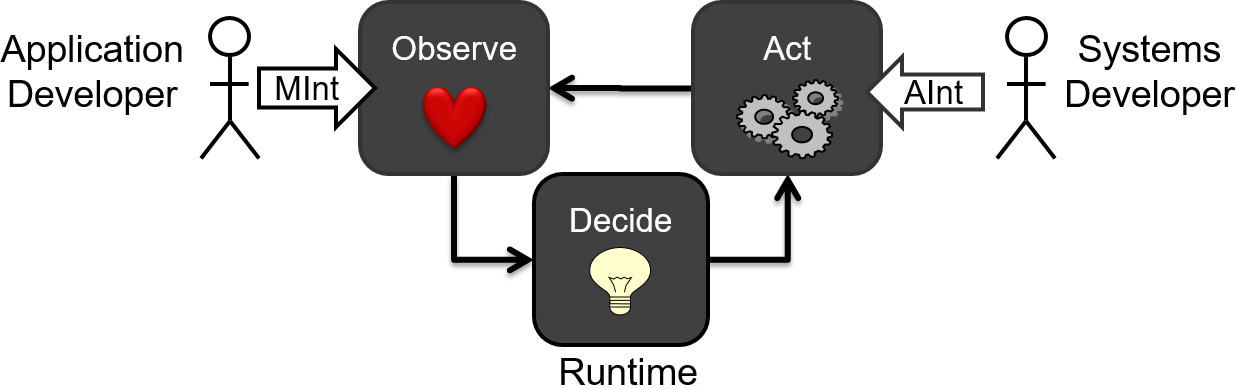
\includegraphics[width=0.6\textwidth]{figs/SEEC.png}
  \caption{A self-aware computing (SEEC) runtime model -- observe, decide, and act.}
  \label{fig:seec}
  \end{centering}
\end{figure}

The lack of both portability and optimality of heuristics demand that we develop more general approaches to addressing the problems in balancing performance and power/energy.
In his PhD dissertation, Hoffmann proposes a ``self-aware'' computing model (SEEC) that uses a closed-loop feedback design to \emph{observe}, \emph{decide}, and \emph{act} \cite{HoffmannPhD}.
\figref{seec} demonstrates this concept.
The SEEC model is more portable than many heuristics because it includes an observation step that measures behavior at runtime rather than relying strictly on assumptions made offline.
We build on this high-level model and use feedback systems that measure application and system behavior during runtime to make informed changes to resource allocations as new information becomes available.
Furthermore, our general feedback system designs do not depend on extremely accurate or complete models.
Instead, they rely on runtime measurements to fine-tune their decisions.


\section{Contributions}

This dissertation addresses two common goals in managing software performance and system energy consumption.
The first is the constrained optimization problem of meeting an application performance goal while minimizing energy consumption.
Software performance constraints are common in applications that run on platforms ranging from embedded to server-class.
% , \eg cloud-based software that must meet quality-of-service guarantees.
The second addresses the problem of running software as energy-efficiently as possible, \ie maximizing the ratio of work completed to energy consumed.
% Maximizing energy efficiency is particularly beneficial in HPC, where systems should be kept busy while reducing the cost of scientific insight.
We address these two problems with three distinct projects:
\begin{itemize}
\item POET, the \textbf{P}erformance with \textbf{O}ptimal \textbf{E}nergy \textbf{T}oolkit: A portable, control-theoretic framework for meeting soft application performance goals while optimizing energy consumption, which we demonstrate by tuning DVFS settings and core allocations.
\item CoPPer, \textbf{Co}ntrol \textbf{P}erformance with \textbf{P}ow\textbf{er}: A model-free, control-theoretic approach for meeting soft application performance constraints by tuning processor power caps and allowing the hardware to optimize energy consumption.
\item CEES, \textbf{C}lassification of \textbf{E}nergy-\textbf{e}fficient \textbf{S}ettings: A machine learning classification framework for predicting energy-efficient system settings based on low-level hardware performance counter metrics, which we demonstrate by tuning DVFS, socket allocations, and the use of HyperThreads.
\end{itemize}
\appref{tools} describes portable tools created to support these projects that we believe are useful to other researchers and developers.
\appref{urls} provides open-source release information for POET, CoPPer, and supporting tools.


\subsection{POET}

POET addresses the problem of meeting soft real-time application performance goals while minimizing energy consumption.
A significant amount of software is subject to performance constraints, from applications running on low-power embedded platforms to those in high-performance, high-power environments like on servers in datacenters.
Optimizing energy consumption increases the usable runtime of battery-powered systems like tablets, smartphones, and smaller devices we now classify as Internet of Things; for always-on devices, it reduces the runtime energy costs.

Kim \etal prove that an optimal solution to this constrained optimization problem requires, at most, two system configurations from the convex hull of the tradeoff space \cite{kim-cpsna2015}.
POET uses control theory to meet the performance goal and linear optimization to select the optimal pair of system configurations that satisfy the performance constraint.
While POET was originally designed for embedded systems \cite{POET}, we later evaluated it on a server-class system \cite{POETMCSoC}.

POET's evaluation uses DVFS and core allocation as the system knobs to control performance and energy consumption.
While significant prior work has used these knobs, their solutions tend to be restricted to particular applications and systems, limiting their portability.
In contrast, POET's design is independent of any particular application or platform and their performance/power tradeoff spaces.

We find that POET achieves:
\begin{itemize}
\item \textbf{Ease of Use}: Integrating POET with applications only requires a few additional lines of code.
\item \textbf{Predictable Performance}: POET meets a range of performance targets, minimizing the error between the goal and the achieved performance.
\item \textbf{Energy Savings}: Using an offline oracle, we verify that POET achieves near-optimal energy consumption (\eg 1.3\% over optimal on an Intel-powered tablet, 2.9\% on an ARM big.LITTLE system), which includes POET's runtime overhead.
\item \textbf{Adaptability}: POET adapts to phases in application and input behavior, achieving increased energy savings during periods of low computational demand.
Additionally, POET adapts to noise in the system introduced by co-scheduled applications to ensure that performance goals are still met when feasible, and makes a best effort otherwise.
\end{itemize}


\subsection{CoPPer}

CoPPer also addresses the problem of optimizing energy consumption under a soft performance constraint, but does so by tuning hardware power caps.
Recent trends suggest that software control of DVFS is being deprecated, making all prior software approaches that depend on DVFS obsolete.
Linux kernel developers have acknowledged this trend \cite{lwn602479}.
In fact, the Linux kernel documentation notes, ``the idea that frequency can be set to a single frequency is fictional for Intel Core processors. Even if the scaling driver selects a single P-State, the actual frequency the processor will run at is selected by the processor itself'' \cite{KernelPstate}.

However, hardware is not aware of application-level performance requirements, so a software component is still needed to ensure that performance constraints are respected.
Fortunately, emerging interfaces let software set \emph{power caps} on hardware, with hardware free to determine what DVFS frequencies should be used and when, so long as the average power over some time window is respected.
For example, Intel's Running Average Power Limit (RAPL) allows software to set power limits on hardware \cite{RAPL}.
This poses a new challenge.
Meeting performance constraints with DVFS is easy: simple linear models map changes in processor clock frequency to changes in application performance.
Meeting performance requirements with power capping is harder: power and speedup have a non-linear relationship (\eqnref{bg-power}) and most applications exhibit diminishing performance returns with increasing clock frequency (and thus power), \ie are not entirely compute-bound.

CoPPer proposes to leverage hardware power capping to control performance, leaving the energy optimization to the hardware.
Its evaluation uses Intel RAPL, which manages DVFS in hardware at finer-grained intervals than software can, while strictly respecting the imposed power limit.
CoPPer makes the following contributions:
\begin{itemize}
\item Demonstrates the need for a DVFS alternative that allows software to manage performance/power tradeoffs.
\item Proposes software-defined power capping as a replacement for software-managed DVFS.
\item Presents CoPPer, a feedback controller that meets performance goals by manipulating hardware power caps, handles non-linearity in power cap/performance tradeoffs, and introduces adaptive \emph{gain limits} to further reduce power when it does not increase performance.
\item Evaluates CoPPer using Intel RAPL on a dual-socket, 32-core server.
We find that CoPPer achieves performance guarantees similar to software DVFS control, but with better energy efficiency.
Specifically, CoPPer improves energy efficiency by 6\% on average with a 12\% improvement for memory-bound applications.
At the highest performance targets, CoPPer's gain limit saves even more energy: 8\% on average and 18\% for memory-bound applications.
\end{itemize}


\subsection{CEES}
\label{sec:intro-ee}

In other scenarios, it is desirable to maximize energy efficiency, \ie complete a fixed-size computation using the least energy possible without a performance constraint.
It is becoming well-established that the \emph{race-to-idle} heuristic is not energy-efficient.
% Our discussion of \emph{race-to-idle} in the context of performance constraints earlier is irrelevant, since if that heuristic cannot meet a constraint, no other approach can.
It may then seem reasonable to simply run in the lowest-power system configuration, but this approach fails to account for elapsed time, so energy consumption may still exceed optimal even when consuming low power.
Identifying the most energy-efficient system setting is challenging since the optimal setting varies depending on varying application resource demands.

We address this problem in the High Performance Computing (HPC) domain.
It has historically been desirable in HPC to run software as fast as possible.
The motivation behind this approach is either to: (1) get an answer to a scientific question as fast as possible, or (2) for the HPC cluster to complete as much work as possible, \ie maximize the cluster throughput.
The goal of completing an application as fast as possible leaves little room for power/energy optimization, although some work has been done in this area (see \secref{related}).
Until recently, maximizing application performance also solved the latter problem.
Now we are moving toward the era of exascale systems with strict power budgets \cite{Exascale20MW}.
Hardware over-provisioning, which allows more systems to operate in a cluster than can actually be supported if each were consuming their maximum power budget, has been proposed as an approach to improve cluster throughput \cite{PatkiRMAP}.
It works because systems do not usually require their maximum allowable power budget.
In these new hardware over-provisioned, power-constrained clusters, maximizing energy efficiency instead of application performance will both decrease the cost of per-application scientific insight and maximize the throughput of the cluster.

Our solution is to treat this challenge as a classification problem, using samples from low-level hardware performance counters to drive machine learning algorithms that predict the most energy-efficient configuration to use.
This approach does not require the software to provide its own instrumentation, nor does the classifier need to know anything about the application in advance.
Using classification instead of estimation reduces the computational overhead of the software solution, at the cost of less insight into the resource predictor's decision.
We tune DVFS, socket allocation, and the use of HyperThreads.

This work makes the following contributions:
\begin{itemize}
\item Proposes optimizing \emph{energy efficiency} instead of \emph{runtime} to decrease the cost of scientific computation.
\item Establishes the problem complexity---of 15 different machine learning classification techniques evaluated, only some are suitable for optimizing energy efficiency.
\item Demonstrates that sufficiently powerful classifiers can dramatically reduce energy consumption by accurately predicting energy-efficient system settings at runtime.
\item Extrapolates from empirical results to posit that optimizing energy efficiency can improve the throughput of hardware over-provisioned, power-constrained systems by up to 24\%.
\end{itemize}

\chapter{Related Work}
\label{sec:related}

This chapter discusses work related to performance, power, and energy awareness.
We first discuss work relating to POET and CoPPer---meeting performance constraints and optimizing energy consumption.
% Research in this area is common in the embedded systems domain, though some work has explored approaches for systems at larger scales.
We then discuss power and energy-aware work in the High Performance Computing domain, where trading performance for power/energy savings is less common.
Finally, we describe research projects by other researchers that build off work in this dissertation.


\section{Performance Constraints and Energy Awareness}

Computing systems are often underutilized, leading to significant portions of time where application performance requirements can be met using less than the full system capacity \cite{google,MeisnerISCA2011}.
This trend has led to flourishing scheduling research that tailors resource usage to meet performance requirements, often while optimizing another dimension like power or energy consumption.
Modern systems expose a variety of configurable resources, which energy-aware schedulers can adjust to tune performance and power behavior.
This flexibility allows the system to adapt to different circumstances or different application needs, but also increases software complexity.
The problem is exacerbated when approaches must achieve portability across a range of different systems, which expose different resources to software and have unique performance/power tradeoff spaces.

% DVFS and core allocation
Software-based DVFS management is essential for many energy-aware scheduling algorithms \cite{Albers,YDS}.
At the processor level, DVFS has been used to meet performance requirements \cite{Lu2002,Wu2004} and implement power capping \cite{lefurgy2008power}.
Allowing DVFS to be set separately on different cores provides further benefits \cite{Isci2006,Rangan2009}.
Similarly, managing DRAM DVFS increases energy efficiency \cite{Memscale,Diniz2007}.
Recent survey papers devote entire sections to the various ways DVFS has been used in scheduling systems \cite{MittalSurvey,ZhuralevSurvey}.
In modern multicore systems, allocating a subset of cores and sockets (with aggressive clock-gating to save power) is also common, and more recently comes with the additional challenge of scheduling for heterogeneous architectures \cite{Petrucci2012}.

% Naive approaches
One simple heuristic for minimizing energy is \emph{race-to-idle}, which allocates all resources until a job completes and then idles the system until the next job arrives \cite{google}.
This heuristic is portable since it does not require knowledge about the system, but empirical studies show that it is not optimal \cite{google,Cheng2009,Yang2007,Yun2010}.
A recent study by Kim \etal demonstrates that an optimal solution requires knowledge of how the different configurable resources in a system affect the specific application under control---information which \emph{race-to-idle} does not use \cite{kim-cpsna2015}.
The same study shows that \emph{race-to-idle} is dominated by a \emph{pace-to-idle} heuristic, \ie \emph{pace-to-idle} is theoretically never worse than \emph{race-to-idle} and can be much better.

% Multiple knobs
It is not surprising that a number of different frameworks have arisen for intelligently controlling multiple resources to minimize energy.
Many empirical studies have shown that it is more energy-efficient to coordinate multiple resources than to manage any one alone \cite{google,Cheng2009,Yang2007,Yun2010}.
Examples include systems that coordinate DVFS with core usage \cite{packandcap-old,TCST,packandcap-new}, coordination of processor and DRAM DVFS \cite{Chen2011,CoScale,Felter2005,Li2007}, and DVFS with thread scheduling \cite{Rangan2009,Winter2010}.
Several other approaches coordinate processor-wide DVFS with adaptations to the memory system and processor pipeline \cite{Bitirgen2008,dubach2010,METE}.
For example, Dubach \etal coordinate several microarchitectural features~\cite{dubach2010},
Petrucci \etal coordinate thread scheduling and the use of heterogeneous cores \cite{Petrucci2012}, while Maggio \etal coordinate core allocation and clock speed~\cite{TCST}.
Bertini \etal coordinate tiers of a multi-tier webserver for e-commerce \cite{Bertini2007}.
AbouGhazaleh \etal coordinate the speed of the processor and cache \cite{AbouGhazaleh2007}, while Yun \etal also coordinate the speeds of multiple on-chip components \cite{Yun2010}.
Liu \etal coordinate job scheduling and clock speed on clusters \cite{Liu2008}.
Bitirgen \etal coordinate clock speed, cache, and memory bandwidth in a multicore~\cite{Bitirgen2008}.
The METE system manages clock speed, memory bandwidth, and core usage \cite{METE}.
Sinangil \etal co-design a processor architecture which exposes both monitoring and configurable resources with an operating system that dynamically manages those resources \cite{sinangil2014self}.
All of these approaches coordinate multiple resources, but do so using system-specific implementations, \eg METE's controller would have to be redesigned to work with Bitirgen et al.'s architecture.

% Complementary approaches
We also note two approaches that are complementary to POET.
Zhao \etal manage processor speed to meet both reliability and timing constraints with minimal energy \cite{Zhao2012}.
This problem is complicated by the effect DVFS scaling has on hardware reliability.
It is possible that POET's general approach to resources other than DVFS might allow additional energy savings if incorporated in Zhao et al.'s work.
He \etal propose adaptive energy management in the power circuitry itself to meet timing constraints while adapting the delivered energy to increase battery efficiency \cite{He2013}.
It is possible that combining POET's runtime-level resource management with this supply-level approach would further increase efficiency.

% General frameworks for multiple resources
Several frameworks have been proposed to meet real-time constraints by managing multiple resources.
These approaches are typically implemented as middleware that take a specification of available resources and a performance goal, and then meet that goal.
Rajkumar \etal propose a general framework (with system-specific implementation) for allocating resources to achieve real-time requirements, but this approach is not energy-aware \cite{Rajkumar}.
Sojka \etal propose a portable middleware layer for allocating resources to meet soft real-time constraints, but this system does not minimize energy \cite{Sojka}.
ControlWare is another middleware approach that uses control theory to meet quality-of-service constraints, but does not address energy concerns \cite{ControlWare}.

These approaches provide portable real-time guarantees, which is itself a hard problem, but they do not provide energy savings.
LEO is a machine learning system that can meet performance constraints with minimal energy consumption \cite{LEO}.
LEO is very accurate and provides high energy savings, even with no prior knowledge of the application currently running.
Its approach is extremely portable, but also incurs very high overhead.
Interestingly, LEO and POET have complementary weaknesses---POET has low runtime overhead, but requires prior knowledge in the form of a configuration model while LEO has high overhead, but requires no prior knowledge.
Follow-up work to LEO addressed this issue with CALOREE (discussed futher in \secref{related-inspired}) \cite{CALOREE}.
PTRADE also uses control theory to manage general collections of resources \cite{PTRADE}, and is perhaps the most similar to POET.
PTRADE minimizes power consumption, but not necessarily energy.
In addition, PTRADE uses heuristic optimizations, which are not portable, while POET uses a true minimal-energy scheduling algorithm.


\section{High Performance Computing}

Power and energy in HPC systems is a growing concern, though prior work in the area has often not allowed trading performance for power or energy savings.
For example, Adagio uses DVFS to save energy with less than 1\% increase in runtime \cite{RountreeAdagio}.
Other work depends on accurate prediction of a code's critical path to reduce power where it will not slow down an application \cite{Jitter,Marathe2015}.
Patki \etal propose to better utilize available power with hardware over-provisioning to increase total system throughput \cite{PatkiRMAP}.
Sarood \etal have shown similar results: hardware over-provisioning increases performance given a power cap \cite{Sarood2013}.
Hardware over-provisioning acknowledges that compute resources are no longer the primary factor limiting cluster size---power is, allowing us to more aggressively trade performance and power/energy consumption.

Other works demonstrate that low-level hardware performance counters can drive solutions for modeling and improving power/energy consumption \cite{Libutti2014,Sasaki,Chetsa,WuHPCComputer}.
Using Dynamic Concurrency Throttling and DVFS to reduce energy consumption without performance loss, Curtis-Maury \etal use hardware events to create an energy-aware logistic regression model for predicting performance and power \cite{Curtis-Maury2008}.

As the number of system settings increases and their interaction becomes more complicated, several approaches have turned to machine learning to manage them.
Paragon \cite{Paragon} and Quasar \cite{quasar} guarantee quality-of-service constraints in heterogeneous data centers using a scheduler based on the learning system that won the Netflix prize \cite{NetflixPrize}.
LEO (mentioned previously) uses a Hierarchical Bayesian Model to minimize energy for different system utilization requirements \cite{LEO}.
These approaches all estimate the performance and power of every possible system configuration, then search those estimates to find the best configuration that meets their operating constraints.
The need to estimate every configuration's behavior is expensive, requiring half a second \cite{LEO} to several seconds \cite{Paragon} of overhead.
In contrast, our proposed approach simply returns the best system settings without predicting their actual energy efficiency, an approach that requires orders of magnitude less overhead (see \secref{classifiers-eval-overhead}).
Ferroni \etal use classification based on hardware events to select the best power model for an application from a predetermined set, and then assign resources to that application in a multi-tenant virtualized infrastructure \cite{FerroniTACO}.
This approach and our proposed approach are complementary, in that Ferroni \etal assign resources at the node-level, while our proposed approach can fine-tune resource usage within a node.

Our approach for maximizing energy efficiency is most closely related to other node-level approaches for managing performance and energy.
PUPiL maximizes node performance given a power cap by adjusting system settings to the particular needs of an application \cite{pupil}.
Chasapis \etal maximize performance for power-capped NUMA nodes by recognizing the effect that manufacturing variability can have on individual core performance \cite{Chasapis2016}.
Both of these approaches maximize performance for a given power constraint.
Neither, however, is capable of minimizing energy, which requires changing both power and performance as in our proposed approach.
ParallelismDial is a node-level approach for managing application-level parallelism to increase energy efficiency \cite{Sridharan2013}.
ParallelismDial has similar goals to our proposed approach, but they are complementary---it works at the application level, while our approach operates at the system level.
In future work, it would likely be beneficial to combine the two to further reduce overhead and improve energy savings.


\section{Inspired Projects}
\label{sec:related-inspired}

Research in this dissertation, and POET in particular, has been used as the foundation for projects by other researchers.

Farrell and Hoffmann build on POET to create MEANTIME, which provides hard real-time guarantees instead of soft performance guarantees \cite{meantime}.
They use the concept of approximate computing to tune application accuracy when their runtime determines that a performance constraint may not be met.
The approach usually only requires small changes to application accuracy, \eg peak signal-to-noise ratio (PSNR) and the bitrate of a video encoder, while still tuning system-level knobs like in POET to save energy.

Aforementioned work by Mishra \etal combines POET with machine learning in a project called CALOREE, which reduces the amount of offline work needed to generate the controller's resource specification \cite{CALOREE}.
CALOREE uses transfer learning, taking information from both previously seen applications and the current application, to model how interacting resources affect the current application's speedup.
It then makes online updates to the controller's resource specification and pole value using more accurate models.

POET and Bard were also the starting point in an ongoing project called Proteus.
Proteus is developing a programming language called FAST, which allows programmers to provide \emph{intent specifications} instructing the runtime of desired constraints and optimizations.
FAST satisfies these intents by tuning both application and system knobs, \eg to manage application performance, application accuracy, and system power or energy consumption.

\chapter{POET: The Performance with Optimal Energy Toolkit}
\label{sec:poet}

This chapter describes POET (the \textbf{P}erformance with \textbf{O}ptimal \textbf{E}nergy \textbf{T}oolkit).
\secref{related} discussed existing work in managing performance and power/energy awareness.
Like POET, a number of these approaches use feedback control to manage timing constraints \cite{Agilos,Bertini2007,grace2,CoAdapt,Maggio13,TCST,ControlWare,PTRADE,Fu2012,Li2007}.
POET is most related to prior approaches that abstract resource management into a middleware or runtime, like \cite{ControlWare,Sojka,PTRADE,Rajkumar}.
Control techniques provide a formal framework for reasoning about the dynamic behavior of the system.
POET is unique in its energy awareness, in its design for portability, and the incorporation of a true minimal-energy resource allocation algorithm.

\TODO{Combine RTAS and MCSoC papers, including motivation, usage, and evaluation.}

\section{Motivation}
\label{sec:poet-motivation}

To motivate the need for POET, we summarize prior work \cite{Imes2014}.
We evaluate timing and energy tradeoffs on two embedded platforms: a Sony Vaio SVT11226CXB tablet system with an Intel Haswell processor and an ODROID-XU+E ARM big.LITTLE development board.
The two platforms have: (1) different configurable resources for performance/power management, and (2) timing/energy tradeoffs with different topologies.
Resource allocation strategies that save energy on one are wasteful on the other.

\tblref{poet-machines} presents each system's configurable resources.
The Vaio allows configuring the number of active cores, the use of hyperthreads, processor clock speed, and the use of TurboBoost.
The ODROID supports configuring the number of active cores, whether the application uses the ``big'' (Cortex-A15 high-performance, high-power) or ``LITTLE'' (Cortex-A7 low-performance, low-power) cores, and the independent clock speeds of the big and LITTLE clusters.

\begin{table}[t]
\caption{Two embedded platforms with different configurable components.}
\label{tbl:poet-machines}
\tiny
\centering
\begin{tabular}{lcccccccc}
  \textbf{Platform} & 
  \textbf{Processor} &
  \textbf{Cores} & 
  \textbf{Core Types} &
  \textbf{Speeds (GHz)} &
  \textbf{TurboBoost} &
  \textbf{HyperThreads} & 
  \textbf{Num. Configs} \\
  % \textbf{Configurations} \\
  \hline
  \hline
  SVT11226CXB & Intel Haswell  & 2 & 1             & 0.6--1.5          & yes & yes & 46 \\
  ODROID-XU+E & ARM big.LITTLE & 8 & 2 (A15, A7)   & 0.8--1.6, 0.5--1.2 & no  & no  & 70 \\
  \hline 
  \hline
\end{tabular}
% \vskip -.7em
\end{table}

Our example features a video encoder, composed of jobs, where each job encodes a frame.
We instrument the encoder to report the latency and platform energy consumption for each job.
\figref{poet-x264-motivation-tradeoffs} shows the tradeoffs between job latency and system energy consumption for each platform, where each point represents the average behavior of a different configuration.
The x-axis shows latency, normalized to 1---the empirically determined worst case.
The y-axis shows energy, normalized to 1---the highest measured energy.
The tradeoffs are obviously very different for the Vaio and the ODROID.
For the Vaio, energy increases as frame latency increases; \ie a slower job wastes energy.
For the ODROID, energy decreases as frame latency increases; \ie slower encodings save energy.

\begin{figure}[t]
  % \vskip -1.8em
  \centering
  \subfloat[Latency/Energy tradeoffs.]%
  {\begin{tikzpicture}

\definecolor{s1}{RGB}{228, 26, 28}
\definecolor{s2}{RGB}{55, 126, 184}
\definecolor{s3}{RGB}{77, 175, 74}
\definecolor{s4}{RGB}{152, 78, 163}
\definecolor{s5}{RGB}{255, 127, 0}

\begin{groupplot}[
    group style={
        group name=plots,
        group size=1 by 1,
        xlabels at=edge bottom,
        xticklabels at=edge bottom,
        vertical sep=5pt
    },
xlabel={\footnotesize Latency},
xlabel near ticks,
height=4.2cm,
%width=0.5\textwidth,
width = 4.6cm,
xmajorgrids,
ymajorgrids,
grid style={dashed},
xtick={0,0.25,0.5,0.75,1.0},
xticklabels={0,0.25,0.5,0.75,1.0},
xticklabel style={font=\footnotesize},
xmin=0,
xmax=1.1,
yticklabel pos=left,
enlargelimits=false,
tick align = outside,
tick style={white},
xticklabel shift={-5pt},
yticklabel shift={-5pt},
ylabel shift={-2pt},
ylabel style={align=center},
unbounded coords=jump,
]

\nextgroupplot[ylabel={\footnotesize Energy}, 
%ylabel shift={6mm},
ytick={0,0.25,0.5,0.75,1.0},
yticklabels={0,0.25,0.5,0.75,1.0},
yticklabel style={font=\footnotesize},
ymin=0,
ymax=1.1,
legend entries={{Vaio},{ODROID}},
legend style={draw=none,at={(0.5,1.35)},anchor=north,legend columns=4,line width=5pt,font=\footnotesize},
]
\addplot[thick, solid, color=s1, only marks, mark=square*] table[x index=2,y index=5,col sep=tab] {img/poet/tradeoffs-vaio.txt};
\addplot[thick, solid, color=s3, only marks, mark=*] table[x index=2,y index=5,col sep=tab] {img/poet/tradeoffs-odroid.txt};


\end{groupplot}

\end{tikzpicture}
%
  \label{fig:poet-x264-motivation-tradeoffs}}
  \subfloat[Heuristic energy consumption.]%
  {\begin{tikzpicture}

\begin{groupplot}[
    group style={
        group name=plots,
        group size=1 by 1,
        xlabels at=edge bottom,
        xticklabels at=edge bottom,
        vertical sep=5pt
    },
% axis x line* = bottom,
xlabel near ticks,
major x tick style = transparent,
height=4.2cm,
%width=0.95\columnwidth,
width=4.6cm,
xmin=0,
xmax=3,
enlargelimits=false,
tick align = outside,
tick style={white},
ytick=\empty,
xticklabel shift={-5pt},
%x tick label style={rotate=0, anchor=south},
xlabel={\footnotesize Platform},xtick={1,2,3},
xticklabels={
{\scriptsize Vaio},
{\scriptsize ODROID}
},
ymin=1,
ymax=2.25,
ytick={1.0,1.25,1.5,1.75,2.0},
yticklabels={1.00,1.25,1.50,1.75,2.00,2.25},
legend cell align=left, 
legend style={ column sep=1ex },
ymajorgrids,
grid style={dashed},
]
\nextgroupplot[ylabel={\footnotesize Energy},
ybar=\pgflinewidth,
bar width=8pt,
legend entries = {{never-idle},{race-to-idle}},
legend style={draw=none,legend columns=2,at={(0.5,1.35)},anchor=north,font=\footnotesize},
]
\addplot table[x index=0,y index=2, col sep=space] {img/poet/heuristics2.txt};
\addplot table[x index=0,y index=3, col sep=space] {img/poet/heuristics2.txt};


\end{groupplot}

\end{tikzpicture}
%
  \label{fig:poet-x264-motivation-heuristics}}
  \caption{Timing and energy behavior for encoding video on the Vaio and ODROID.}
  \label{fig:poet-x264-motivation}
\end{figure}

The different shapes of these tradeoff spaces lead to different optimal resource allocation strategies.
Empirical studies show that the \emph{race-to-idle} heuristic, which makes all resources available and then idles after completing a job, is near-optimal on systems like the Vaio~\cite{google,Hoelzle2009,HotPower,Imes2014,PowerSlope}.
On systems like the ODROID, recent approaches save energy by keeping the system constantly busy, like the \emph{never-idle} heuristic~\cite{Carroll13,HotPower,Imes2014,LeSueur11,Lin2010}.

To demonstrate the importance of choosing the right strategy, we analyze the two heuristics on both platforms and compare their energy consumption to optimal (found by measuring every possible resource configuration).
We set a latency target equal to twice the minimum latency and measure the energy consumption of encoding 500 video frames using each heuristic.
\figref{poet-x264-motivation-heuristics} shows the results, normalized to optimal.
Both heuristics meet the latency target, but their energy consumptions vary tremendously.
On the Vaio, \emph{race-to-idle} is near-optimal, but \emph{never-idle} consumes 13\% more energy.
Conversely, \emph{never-idle} is near-optimal for the ODROID, but \emph{race-to-idle} consumes $2 \times$ more energy.

These results demonstrate that resource allocation strategy greatly affects energy consumption, and more importantly, that heuristic solutions are not portable across systems.
These two points motivate the need for an approach like POET, which provides near-optimal resource allocation while remaining platform-independent.
% POET's runtime uses control theory to meet timing constraints and linear programming to minimize energy consumption.
% A POET user does not need to be a control or optimization expert, but simply make small changes to their application code.
% POET makes it easy for embedded developers to write portable applications providing predictable timing and minimal energy across a range of devices.

\section{General and Portable Resource Allocation}
\label{sec:poet-framework}

The goal of POET's resource allocation framework is twofold.
First, it must provide predictable timing so application jobs meet their deadlines.
Second, it should minimize energy consumption given the timing requirement.
While these two subproblems are intrinsically connected, they can be decoupled to provide a general solution.
The complexity arises from the need to keep resource allocation general with respect to the running application and the hardware platform.
We tackle the problem of providing predictable timing using control theory by computing a \emph{generic control signal}.
Using the computed control signal, we then solve the energy minimization problem using mathematical optimization.

\figref{poet-runtime} illustrates our approach.
The \textbf{application} informs the runtime of its job \emph{performance goal}.
Measuring each job start and completion time (\emph{performance feedback}), POET's runtime computes the \emph{performance error} and passes it to the \textbf{controller}.
The controller uses the error to calculate a \emph{generic control signal}, indicating how much the application speed should be altered.
This signal is used by the \textbf{optimizer}, together with the \textbf{resource specification}, to produce a \emph{resource schedule} that achieves the desired performance goal while minimizing energy consumption.
Both the controller and the optimizer are designed independently of any particular application and system.
The only assumption made is that applications are composed of repeated jobs with a soft real-time performance goal.
% As we target multicore platforms, we assume each job may be processed by multiple, communicating threads.

\begin{figure}[t]
  \centering
  \tikzset{%
  app/.style    = {draw, thin, rectangle, minimum height = 2em,
    minimum width = 2em, fill=black!25},
  block/.style    = {draw, thick, rectangle, minimum height = 2.5em,
    minimum width = 2.5em},
  blockres/.style    = {draw, thick, rectangle, minimum height = 2.5em,
    minimum width = 2.5em, fill=green!25},
  biblock/.style  = {draw, thick, rectangle, minimum height = 5.5em,
    minimum width = 6em, fill=red!25},
  sum/.style      = {draw, circle, node distance = 2cm}, % Adder
  input/.style    = {coordinate}, % Input
  output/.style   = {coordinate} % Output
}

\begin{tikzpicture}[scale=1.0,transform shape, auto, thick, node distance=1.5cm, >=triangle 45]

\draw
  % Drawing the top blocks
  node [input, name=goalaccuracy] {} 
  node [left of=goalaccuracy, node distance=0.35mm]{}
  node [sum, right of=goalaccuracy] (sumaccuracy) {} % negative feedback
  node [block, right of=sumaccuracy, align=center, node distance=3.5cm] (controlaccuracy) 
    {Controller}
  node [block, right of=controlaccuracy, align=center, node distance=4.2cm] (translateaccuracy) 
    {Optimizer}
  node [blockres, above of=translateaccuracy, align=center, node distance=1.8cm] (resourcefile) 
    {Resource\\Specification}
;
  % Connectng lines
\draw[->](goalaccuracy) -- node[align=center] {Performance\\Goal}(sumaccuracy);
\draw[->](sumaccuracy) -- node[align=center] {Performance\\Error}(controlaccuracy);
\draw[->](controlaccuracy) -- node[align=center] {Generic\\Control\\Signal}(translateaccuracy);
\draw[->](resourcefile) -- (translateaccuracy);

% Draw software system
\draw
  node [biblock, right of=translateaccuracy, node distance=4.5cm, align=center] (system)
    {\\System\\\\\\}
;
\draw
  node [app, right of=translateaccuracy, node distance=4.5cm, align=center, yshift=-0.5cm] (software)
    {Application}
;

% lines from translators to software
\draw[->](translateaccuracy.east) -- node [name=ka,align=center]{Resource\\Schedule} (translateaccuracy.east -| system.west);

% Connectng lines
\coordinate (feedbackup) at ([yshift=-0.6cm]sumaccuracy.south);
\draw (software.west |- feedbackup) -| node [near end,align=center] {Performance\\Feedback} (feedbackup);
\draw[->](feedbackup) -- node[pos=0.99] {$-$} (sumaccuracy);

\end{tikzpicture}
  % \vskip -.5em
  \caption{Overview of the POET runtime.}
  \label{fig:poet-runtime}
% \vskip -.3em
\end{figure}


\subsection{Controller}

The application provides a \emph{performance goal} (work rate) $R_{ref}$, which is easily computed from a workload size (number of jobs) $\omega$ and desired latency goal (deadline) $\tau$ for those $\omega$ jobs:
\begin{equation}
  R_{ref} = \frac{\omega}{\tau}
  \label{eqn:poet-latency-to-performance}
\end{equation}
The controller cancels the error between the desired performance, $R_{ref}$, and the measured performance, $r_m(t)$, which it models as:
\begin{equation}
r_m(t) = s(t-1) \cdot b_r(t-1)
\label{eqn:poet-performance}
\end{equation}
The error $e_r(t)$ is then easily computed as:
\begin{equation}
e_r(t) = R_{ref} - r_m(t)
\label{eqn:poet-error}
\end{equation}
The controller performs its calculations at discrete work (job) intervals to produce a new desired speedup, $s(t)$, implementing the \emph{integral control law}~\cite{Hellerstein2004a}:
\begin{equation}
  s(t) = s(t-1) + (1-\alpha) \cdot \frac{e_r(t)}{b_r(t)}
  \label{eqn:poet-control}
\end{equation}
where $\alpha$ is a \emph{pole} of the closed loop characteristic equation~\cite{ICSE2014} such that $\alpha$ lies within the unit circle:
\begin{equation}
  0 \le \alpha < 1
  \label{eqn:pole}
\end{equation}
The pole is configurable.
Small $\alpha$ values make the controller highly reactive, while large values make it slow to respond to external changes.
However, a large $\alpha$ ensures robustness with respect to transient fluctuations and may be beneficial for very noisy systems.
A small $\alpha$ will cause the controller to react quickly, potentially producing a noisy control signal.

The parameter $b_r(t)$ represents the application's base speed, which directly influences the controller.
Different applications will have different base speeds.
Applications may also experience \emph{phases}, where base speed changes over time.
To accommodate these situations, POET continually estimates base speed using a Kalman filter~\cite{welch2006kalman}, which adapts $b_r(t)$ of \eqnref{poet-control} to the current application behavior.
Assuming minimal measurement variance (\ie even if an application is noisy, the signaling framework does not add additional noise) and denoting the application timing variance as $q_b(t)$, the Kalman filter formulation is standard:
\begin{equation}
\left \lbrace
\begin{array}{rcl}
\hat{b}^{-}(t) & = & \hat{b}(t-1) \\
e^{-}_{b}(t) & = & e_{b}(t-1) + q_b(t) \\
k_b(t) 
  & = & \frac{e^{-}_{b}(t) \cdot s(t)}{[s(t)]^2
        \cdot e^{-}_{b}(t)} \\
\hat{b}(t) 
  & = & \hat{b}^{-}(t) + k_b(t) 
        \, \left[ r_m(t) - s(t) \cdot \hat{b}^{-}(t) \right] \\
e_{b}(t) & = & [1 - k_b(t) \cdot s(t-1)] \, e^{-}_{b}(t)
\end{array}
\right .
\label{eqn:kalman-filter}
\end{equation}
This formulates Kalman gain for job latency as $k_b(t)$, the \emph{a priori} and \emph{a posteriori} estimates of the base speed as $\hat{b}^{-}(t)$ and $\hat{b}(t)$, and the \emph{a priori} and \emph{a posteriori} estimates of the error variance as $e^{-}_{b}(t)$ and $e_{b}(t)$.
The Kalman filter produces a statistically optimal estimate of the system's parameters and is provably exponentially convergent~\cite{CaoSchwartz2003}.

Unlike prior work, the POET controller does not reason about a particular set of resources, but computes a generic control signal $s(t)$.
The advantage of using the Kalman filter is that POET's formulation is independent of particular applications and systems.
POET provides formal guarantees about its steady-state convergence and robustness without requiring users to understand control theory or Kalman filtering---$s(t)$ is computed by the controller, $r_m(t)$ and $q_b(t)$ are measured, and all other parameters are derived.


\subsection{Optimizer}
\label{sec:poet-optimizer}

The optimizer turns the generic control signal computed by the controller into a system-specific resource allocation strategy, translating the speedup $s(t)$ computed with \eqnref{poet-control} into a \emph{schedule} for the available resources.
The \emph{schedule} is computed for the next $\omega$ work units (jobs).

As shown in \figref{poet-runtime}, the optimizer takes, as input, a resource specification containing the set of available system configurations.
There are $C$ possible configurations in the system and by convention, we number the configurations from $0$ to $C-1$.
We use $c = 0$ to indicate the configuration where the least amount of resources is given to the application. %, corresponding to a low-power idle state or sleep state when available.
In contrast, configuration $C-1$ maximizes the resource availability.
Each configuration $c$ is associated with performance and power values, speedup $s_c$ and powerup $p_c$ respectively, which are normalized to $c = 0$.

Given this information, POET solves the following optimization problem:
\begin{eqnarray}
\minimize && \sum_{c=0}^{C-1} \tau_c \cdot p_c \label{eqn:poet-power} \\
\st %&& \nonumber\\
&& \sum_{c=0}^{C-1} \tau_c \cdot s_c \cdot b_r(t) =  \omega \label{eqn:poet-work} \\
&& \sum_{c=0}^{C-1} \tau_c =  \tau \label{eqn:poet-deadline} \\
&& 0 \le \tau_c \le \tau, \qquad \forall c \in \{0,\ldots,C-1\} \label{eqn:poet-time}
\end{eqnarray}
\eqnref{poet-power} minimizes the total energy consumption.
\eqnref{poet-work} constrains all jobs to complete in the next control period.
\eqnref{poet-deadline} ensures that the time is fully scheduled and \eqnref{poet-time} imposes that a non-negative time is assigned to each configuration.
Solving linear optimization problems is, in general, hard, but this particular problem has a structure that makes it practical to solve.
Feasible solutions are confined to a polytope in the positive quadrant defined by the two constraints \eqnsref{poet-work}{poet-deadline}.
Thus, linear programming theory states an optimal solution exists for this problem when all the $\tau_c$ are equal to zero except for (at most) two configurations~\cite{LP}.

\begin{algorithm}[t]
  \caption{Finding a Minimal-Energy Schedule.}
  \begin{algorithmic}
    \footnotesize
    \Require $C$ \Comment{system configurations, given by user}
    \Require $\omega$ \Comment{discrete work units, given by application}
    \Require $s(t)$ \Comment{speedup, given by \eqnref{poet-control}}
    \State $U = \{c \mid s_c \le s(t) \}$
    \State $O = \{c \mid s_c > s(t)\}$
    \State $candidates = U \times O = \{\langle u, o \rangle \mid u \in U, o \in O\}$
    \State $energy = \infty$
    \State $optimal = \langle -1, -1 \rangle$
    \State $schedule = \langle -1, -1 \rangle$ \newline
    \For {$\langle u, o \rangle \in candidates$} \Comment{loop over all pairs}
    \State $\omega_u = \omega \cdot \frac{s_u \cdot (s_o - s(t))}{s(t) \cdot (s_o - s_u)}$ \Comment{compute the work units to spend in each configuration in pair}
    \State $\omega_o = \omega - \omega_u$
    \State $newEnergy = \omega_u \cdot p_u + \omega_o \cdot p_o$ \Comment{compute energy of this pair}
    \If {$newEnergy < energy$} \Comment{compare energy to best found so far}
    \State $energy = newEnergy$
    \State $optimal = \langle u, o \rangle$
    \State $schedule = \langle \omega_u,\omega_o \rangle$
    \EndIf
    \EndFor \newline \newline
    \Return $optimal$ \Comment{pair of configurations with minimal energy} \newline
    \Return $schedule$ \Comment{work units to spend in each configuration}
  \end{algorithmic}
  \label{algo:poet-optimal}
\end{algorithm}

\algoref{poet-optimal} takes the set of configurations $C$, the controller's speedup $s(t)$, and the number of work units $\omega$ in a control period.
It then divides the configurations in two distinct subsets.
The first subset contains all configurations with a speedup less than or equal to the target.
The second contains the remaining configurations, \ie those with speedups greater than required.
Subsequently, \algoref{poet-optimal} loops over all feasible pairs of configurations, with one from each subset, to determine how much time should be spent in each configuration given speedup constraint.
If the energy of the pair is lower than any previous energy, the algorithm stores the current best pair, its energy, and its schedule.
When the algorithm terminates, its output is the pair of chosen configurations and their assigned times.
The algorithm tests all possible pairs from the two subsets, each of which contains at most $C$ elements, so an upper bound to the algorithm complexity is $O(C^2)$.
We know that there is an optimal solution to the linear program with at most two non-zero $\tau_c$ (as the dual problem has two dimensions \cite{LP}).
Therefore, \algoref{poet-optimal} will find a minimal-energy schedule.


\subsection{Generality and Robustness}

The controller and the optimizer both reason about speedup instead of absolute performance or latency.
The absolute performance of the application, measured by the average latency of its jobs, will vary as a function of the application itself and the platform it executes on.
However, speedup is a general concept and can be applied to any application and system, providing a more general metric for control.
Moreover, the controller customizes the behavior of a specific application using the estimate of its base speed produced by the Kalman filter
The optimizer operates in a platform-independent manner, using the available configurations provided as input to find the optimal solution, without relying on a particular heuristic that may be system-specific or application-dependent.
Finally, the customizable pole $\alpha$ in \eqnref{poet-control} allows for flexibility and robustness to inaccuracies and noise.

The ability to control robustness to inaccuracies and model errors is a major advantage of feedback control systems~\cite{ICSE2014}.
In particular, POET is stable and converges to the desired latency without oscillations provided that $0 \le \alpha < 1$.
Formal analysis of this behavior can be obtained by applying standard control techniques---see the original POET publication for further details \cite{POET}.

In addition to provable convergence, the control formulation allows us to analyze POET's robustness to user error.
In particular, suppose $\Delta$ is a multiplicative error term, indicating the largest error in the speedup values provided in the system configurations.
That is, if the provided speedup is $s_p$, the real value is $s_p \cdot \Delta$.
POET cancels the error despite inaccurate information if and only if $0 < \Delta < \frac{2}{1-\alpha}$.
The value of $\alpha$ therefore determines how robust POET is to errors in speedup specifications.
For example, when $\alpha = 0.1$, $s_p$ can be off by a factor of $2$ and the system is still guaranteed to converge.
Users who can provide good system models will therefore use a small $\alpha$, while less confident users can select a larger $\alpha$.
All the experiments in our evaluation use $\alpha=0$ to test our implementation in the least forgiving setting.
A detailed analysis of POET's robustness is presented in the original POET publication \cite{POET}.

\section{Implementation}
\label{sec:poet-implementation}

We describe how the framework in the previous section is realized in a C library.
We specify the information that must be provided by POET's users, describe the library interface, and then discuss the implementation of the runtime engine.

\subsection{External Inputs}

POET requires three pieces of information from users.
First, it needs the available system configurations and their associated timing and power characteristics.
Second, it needs a means to measure timing and power consumption during runtime.
Third, it requires the application to specify the desired latency target.

The first input is the specification of available system configurations.
POET separates the system configurations into two data structures.
The first is system-agnostic and contains a configuration identifier along with \textbf{speedup} and \textbf{powerup} values.
The second is system-specific and can take any form a developer considers appropriate to define a system configuration.
To simplify the programmer's job, POET includes a default format for this second structure which contains a configuration identifier, the DVFS frequency to apply, and the number of cores to use.
Snippets of actual configuration files representing both these data structures are presented in \figref{config-examples}.
\secref{poet-usage} describes how to characterize a system's timing and power behavior.
These results can be used to create configurations if they are not already available.

\begin{figure}[t]
\centering
\begin{minipage}{.45\columnwidth}
\lstset{
  belowskip=0pt,
  aboveskip=0pt,
}
\begin{lstlisting}[frame=tlr,%
  caption={System-agnostic.},%
  label={lst:control_config_example}]%

#id        speedup         powerup
0          1               1
1          1.20            1.09
2          1.40            1.16
3          1.60            1.30
4          2.12            1.35
5          2.53            1.50
6          2.88            1.64
7          3.18            1.69
\end{lstlisting}
\end{minipage}
% \hfill
\hspace*{0.4cm}
\begin{minipage}{.45\columnwidth}
\lstset{
  belowskip=0pt,
  aboveskip=0pt,
}
\begin{lstlisting}[frame=tlr,%
  caption={System-specific.},%
  label={lst:cpu_config_example}]%

#id        frequency        cores
0          250000           0
1          300000           0
2          350000           0
3          400000           0
4          250000           1
5          300000           1
6          350000           1
7          250000           2
\end{lstlisting}
\end{minipage}
% \vskip -1.5em
\caption{Example of POET configuration files.}
\label{fig:config-examples}
\end{figure}

To measure both latency and power, we modify the Heartbeats API \cite{PTRADE} to record power data along with timing statistics.
We then modify applications to issue heartbeats at appropriate points during processing, typically after the completion of every job.
The issued heartbeats contain power and timing data that POET queries at runtime.

The third necessary input is a latency target.
The user provides the target through the Heartbeats API, specifying a minimum and maximum latency goal.
The timing targets can change during runtime, and POET will take care of the adaptation automatically.


\subsection{Software Interface}
\label{sec:poet-interface}

Users interact with only three POET functions.
\function{poet\_init} initializes POET and returns a \variable{poet\_state} data structure reference.
\function{poet\_apply\_control} executes the controller, runs \algoref{poet-optimal}, and configures the platform.
\function{poet\_destroy} cleans up the \variable{poet\_state} data structure.

POET's initialization function takes, as parameters, references to: the heartbeat data structure used to store the timing and power of the application, the system's configurations, and the function that applies the given system configurations.
It also receives an optional reference to the function that determines the system's current state and a log file name.
The first system configuration data structure (system-agnostic) is of type \variable{poet\_control\_state\_t}, and the second (system-specific) has type \variable{void}.

The two functions passed by reference are the only ones that need to know the format of the second data structure and are therefore passed the \variable{void} type reference given to \function{poet\_init} as parameters.
The first of these two functions must have a signature that matches the \variable{poet\_apply\_func} definition and the second must match the \variable{poet\_curr\_state\_func} definition.

The other two API functions, \function{poet\_apply\_control} and \function{poet\_destroy}, take the \variable{poet\_state} reference as their only parameter.
This variable contains all the control state required to implement the framework described in \secref{poet-framework}.

Auxiliary functions are also provided to load system configurations from files, discover the initial system configuration, and apply system configurations.
The latter two of these meet the \variable{poet\_curr\_state\_func} and \variable{poet\_apply\_func} definitions, respectively, and can be passed to \function{poet\_init}.
These auxiliary functions are platform-dependent and thus kept separate to maintain portability, allowing users to easily substitute their own versions.
They are, however, generic enough that most Linux users do not need to write their own.


\subsection{Runtime}

After an application signals its power and latency with a heartbeat, it makes a call to \function{poet\_apply\_control}, which contains POET's core logic.
Heartbeats are initialized with a {\em window size} value that indicates the number of jobs to complete in a given {\em time interval}.
The window size is analogous to $I(t)$ from \eqnref{poet-work}, while the time interval is equivalent to $\tau$ from \eqnref{poet-time} and \algoref{poet-optimal}.
At the completion of a window, the POET runtime calculates the estimated base speed with \eqnref{kalman-filter}, then computes the latency error with \eqnref{poet-error}.
It subsequently applies the controller of \eqnref{poet-control} to determine the speedup necessary to eliminate the computed error.
Finally it determines the energy-minimal resource schedule that achieves the necessary speedup using \algoref{poet-optimal} and applies the first configuration in the schedule by executing the provided \variable{poet\_apply\_func} function.

The last step, a call to the \variable{poet\_apply\_func} specified by the user, is a platform-dependent operation.
For example, the function included with POET for Linux platforms invokes the \app{taskset} utility to force the process and all of its threads onto the desired number of cores and uses the \app{cpufrequtils} interface to adjust the cores' clock speeds.
Developers can specify their own function.
For example, a system may require a different approach to change the number of active cores.
Also, a system may have additional configurable resources that could be adjusted, like memory and network bandwidth.

The only remaining task is to apply the second configuration in the schedule at the appropriate time during the next window.
When the computed number of heartbeats to wait passes, the \variable{poet\_apply\_func} function executes again, but no further computation is performed.
At the completion of the heartbeat window, the control process repeats.

The code snippet shown in \lstref{poet-example} provides an example of application code, highlighting the POET function calls.
% Adding POET to existing applications does not require many modifications to the original code.
The complete modification of an existing application requires nine function calls plus associated variable declarations, for a total of 14 lines of code.
The user provides a desired latency target via the Heartbeats API using the \variable{min\_heartrate} and \variable{max\_heartrate} variables, which represent a desired minimum and maximum speed in terms of jobs completed per second.
POET simply takes the average of these two values, meaning they can be the same.
Given $I(t)$ jobs in a window and a target latency $\tau$, the desired rates are easily computed as:
\begin{equation}
  min\_heartrate = max\_heartrate = \frac{I(t)}{\tau} 
  \label{eqn:latency-to-performance}
\end{equation}
As demonstrated below, Heartbeats initialization also accepts requests for minimum and maximum accuracy and power -- POET does not use these, so they can safely be set to any value.
When initializing POET, the user should specify the system's configurations, encoded in \variable{control\_states} and \variable{cpu\_states}.

\lstset{emph={%  
    poet_state, poet_init, poet_apply_control, poet_destroy%
    },emphstyle={\color{black}\bfseries\underbar}%
}%
\begin{lstlisting}[language=C,%
  caption={Example of POET application code.},%
  label={lst:poet-example}]%

// initialization
heartbeat_t* heart =
  heartbeat_acc_pow_init(window_size, buffer_depth, "heartbeat.log",
                         min_heartrate, max_heartrate, min_accuracy, max_accuracy,
                         1, hb_energy_impl_alloc(), min_power, max_power);
get_control_states(NULL, &control_states, &nstates);
get_cpu_states(NULL, &cpu_states, &nstates);
poet_state* state = poet_init(heart, nstates, control_states, cpu_states,
                              &apply_cpu_config, &get_current_cpu_state,
                              buffer_depth, "poet.log");
// execution of main loop
while(running) {
  heartbeat_acc(heart, count++, 1);
  poet_apply_control(state);
  doWork();
}
// cleanup
poet_destroy(state);
free(control_states);
free(cpu_states);
heartbeat_finish(heart);
\end{lstlisting}

\TODO{Also present updated interface?}

\section{Experimental Design}
\label{sec:poet-usage}

This section details the applications used to evaluate POET and the different evaluation platforms.
The evaluation is broken down into two categories: an embedded systems evaluation and a server-class system evaluation.


\subsection{Applications}

To represent a wide variety of embedded applications, we use eight different benchmarks, none of which were originally written to provide predictable timing.
We choose applications that do not enforce any timing guarantees to challenge POET's approach as much as possible.

The first five applications are included in the PARSEC benchmark suite~\cite{parsec}.
Specifically, we use \app{blackscholes}, \app{bodytrack}, \app{facesim}, \app{ferret}, and \app{x264}.
\app{Bodytrack} and \app{x264} process video input and could be required to match the frame rate of a live feed (\eg from an on-board camera).
\app{Ferret} is a toolkit for content-based similarity search of non-text data and should satisfy a latency requirement on how fast results are returned to users.
\app{Facesim} creates realistic animations of a human face from a model and time sequence of muscle movements, and must maintain a real-time frame rate.
The sixth and seventh applications are \app{dijkstra} and \app{sha}, from the ParMiBench benchmark suite~\cite{parmibench}.
\app{Dijkstra} computes single-source shortest paths in a graph (we use the parallelized multiple queue implementation).
\app{SHA} (Secure Hash Algorithm) is used for secure storage and transmission of data and must maintain response time to ensure timely communication.
The last application is \app{STREAM}~\cite{stream}, a synthetic benchmark for measuring sustainable memory bandwidth, representing a variety of memory-bound applications.

All benchmarks are modified as discussed in~\secref{poet-implementation}, adding Heartbeats and POET calls.
All application inputs used are packaged with the original benchmarks, with the exception of the \app{x264} input which comes from a set of standard test sequences.


\subsection{Evaluation Platforms}

The first part of the evaluation uses two modern embedded devices with different hardware---a Sony VAIO SVT11226CXB tablet PC with a mobile Intel Haswell processor, and a Hardkernel ODROID-XU+E ARM big.LITTLE development platform.
We selected these two platforms because prior work has shown that they expose different timing and energy tradeoffs~\cite{Imes2014}.
% \tblref{poet-embedded-systemknobs} shows the hardware details for both, highlighting the configurable resources, the cardinality of the set of alternatives for each, and the maximum speedup achievable by manipulating that resource alone.
Both platforms run Ubuntu Linux 14.04 LTS.
The Vaio uses kernel 3.13.0, while the ODROID runs kernel 3.4.104.

% \begin{table}[t]
% \caption{Embedded system configurations.}
% \centering
% \begin{tabular}{clcc}
%   & \textbf{Resource} & \textbf{Settings} & \textbf{Max Speedup} \\
% \hline
% \hline
%   \multirow{3}{*}{\begin{turn}{90}\textbf{Vaio}\end{turn}} 
%   & cores        &  2 & 1.81 \\
%   & core speeds  & 11 & 2.72 \\
%   & hyperthreads &  2 & 1.10 \\ 
% \hline
% \hline
%   \multirow{4}{*}{\begin{turn}{90}\textbf{O-XU+E}\end{turn}} 
%   & big cores          & 4 & 6.10 \\
%   & big core speeds    & 9 & 1.97 \\
%   & LITTLE cores       & 4 & 3.94 \\
%   & LITTLE core speeds & 8 & 2.40 \\
% \hline
% \hline
% \end{tabular}
% \label{tbl:poet-embedded-systemknobs}
% \end{table}

The second part of the evaluation uses a dual-socket server system, where each socket contains 8 cores.
With HyperThreading, the system exposes 32 virtual cores.
There are 16 DVFS settings available, including TurboBoost.
The server system also runs Ubuntu 14.04 LTS with Linux kernel 3.13.0.

A \textbf{configuration} is a unique combination of allowable values for the system resources.
In all cases, \app{cpufrequtils} controls processor clock speeds and \app{taskset} controls core allocation.
While the Vaio claims to support different frequency settings on different virtual cores, our experience leads us to conclude that this is not the case.
Thus, we allow only configurations where all cores are set to the same frequency.
The ODROID's version of the Exynos5 Octa does not support executing on the big and LITTLE clusters simultaneously, and all cores in a cluster must operate at the same frequency.
We use a mainline Linux kernel with the default In Kernel Switcher for managing cluster migration.
%IKS maintains compatibility with existing schedulers by modifying existing DVFS systems, but at a cost of supporting execution on only one cluster at a time. This is achieved on the ODROID by using dummy frequency values for the LITTLE cores so as not to overlap with the frequencies provided by the big cores.
On the server system, we set the DVFS frequency on all cores, like on the Vaio.

\begin{table}[t]
\small
\centering
\caption{System power characteristics.}
\begin{tabular}{cccc}
  \textbf{System} & \textbf{Idle Power} & \textbf{Min Power} & \textbf{Max Power} \\
  \hline
  \hline
  Vaio        & 2.50 W  & 3.04 W  & 8.05 W \\
  ODROID-XU+E & 0.12 W  & 0.17 W  & 8.14 W \\
  Server      & 17.90 W & 37.80 W & 199.26 W \\
  % ODROID-XU3  & 0.21 W  & 0.19 W  & 6.37 W \\
  \hline
  \hline
\end{tabular}
\label{tbl:poet-power}
\end{table}

Capturing power/energy metrics naturally requires hardware resources that expose power or energy data to software.
To capture power measurements on the Vaio and the server system, we use the Model-Specific Registers (MSRs) provided by Intel~\cite{SandyBridge}.
On the ODROID, we poll INA-231 power sensors to capture power data for the A15 and A7 clusters as well as for the DRAM and for the GPU~\cite{ina231}.
Basic power figures for the three platforms are shown in~\tblref{poet-power}.
The modified version of Heartbeats includes energy readers for some common hardware (\eg the MSR) and exposes a simple interface for extending to new hardware.
Collecting power data on new platforms with different power or energy monitors is easy and does not require any modifications to POET.

\begin{table}[t]
\small
\centering
\caption{Embedded systems evaluation inputs and configuration details.}
\begin{tabular}{cccc}
  \textbf{Application} & \textbf{Input} & \textbf{Jobs} & \textbf{Window Size} \\
  \hline
  \hline
  blackscholes   & 1 million options              & 400 batches   & 20 \\
  bodytrack      & sequenceB                      & 261 frames    & 20 \\
  facesim        & Storytelling                   & 100 frames    & 20 \\
  ferret         & corel:lsh                      & 2,000 queries & 20 \\
  x264           & ducks\_take\_off               & 500 frames    & 20 \\
  dijkstra       & input\_small                   & 1,000 paths   & 20 \\
  sha            & in\_file(1-16)                 & 1,000 hashes  & 50 \\
  STREAM         & self-generated                 & 1,000 updates & 50 \\
  \hline
  \hline
\end{tabular}
\label{tbl:poet-embedded-inputs}
\end{table}

\begin{figure}[t]
  \centering
  \begin{tikzpicture}

\begin{groupplot}[
    group style={
        group name=plots,
        group size=1 by 1,
        xlabels at=edge bottom,
        xticklabels at=edge bottom,
        vertical sep=5pt
    },
%axis x line* = bottom,
xlabel near ticks,
major x tick style = transparent,
xlabel={},
height=3.5cm,
width=0.95\columnwidth,
xmin=0,
xmax=9,
enlargelimits=false,
tick align = outside,
tick style={white},
ytick=\empty,
xticklabel shift={0pt},
x tick label style={rotate=35, anchor=east, font=\scriptsize},
xtick={1,2,3,4,5,6,7,8,9},
xticklabels={
{blackscholes},
{bodytrack},
{facesim},
{ferret},
{x264},
{dijkstra},
{sha},
{STREAM}},
ymin=0,
ymax=0.6,
ytick={0,0.15,0.30,0.45,0.60},
yticklabels={0,0.15,0.30,0.45,0.60},
legend cell align=left,
legend style={ column sep=1ex },
ymajorgrids,
grid style={dashed},
ylabel shift={0mm},
ylabel style={align=center},
]
\nextgroupplot[ylabel={\footnotesize Coeff. of Variation \\ \scriptsize (Std. Deviation/Mean)},
ybar=\pgflinewidth,
bar width=8pt,
legend entries = {{Vaio},{ODROID-XU+E}},
legend style={draw=none,legend columns=2,at={(0.5,1.4)},anchor=north,font=\footnotesize},
]
\addplot table[x index=0,y index=3, col sep=tab] {img/poet/variability-embedded.txt};
\addplot table[x index=0,y index=2, col sep=tab] {img/poet/variability-embedded.txt};


\end{groupplot}

\end{tikzpicture}

  \caption{Embedded systems application latency variability.}
  \label{fig:poet-embedded-variation}
\end{figure}

\tblref{poet-embedded-inputs} shows the inputs used for each of the applications on the embedded platforms.
We quantify this inherent unpredictability by measuring the latency of each job and computing the coefficient of variation (ratio of standard deviation to the mean) over all jobs in an application.
\figref{poet-embedded-variation} demonstrates this unpredictability for each application when running without POET.
The figure shows that our applications have a range of natural behavior from low variance (implying natural predictability, \eg \app{blackscholes}) to high variance (meaning that the application naturally has widely distributed latencies, \eg \app{x264}).
The variability in the applications is largely the same across platforms, indicating that it is a fundamental property of the applications and not the devices.

\begin{table}[t]
\small
\centering
\caption{Server-class system evaluation inputs and configuration details.}
\begin{tabular}{cccc}
  \textbf{Application} & \textbf{Input} & \textbf{Jobs} & \textbf{Window Size} \\
  \hline
  \hline
  blackscholes   & 10 million options             & 400 batches   & 50 \\
  bodytrack      & sequenceB                      & 261 frames    & 50 \\
  facesim        & Storytelling                   & 100 frames    & 20 \\
  ferret         & corel:lsh                      & 2,000 queries & 50 \\
  x264           & rush\_hour                     & 1,500 frames  & 100 \\
  dijkstra       & input\_large                   & 1,000 paths   & 50 \\
  sha            & in\_file(1-16)                 & 1,000 hashes  & 50 \\
  STREAM         & self-generated                 & 1,000 updates & 50 \\
  \hline
  \hline
\end{tabular}
\label{tbl:poet-server-inputs}
\end{table}

\begin{figure}[t]
  \begin{tikzpicture}

\begin{groupplot}[
    group style={
        group name=plots,
        group size=1 by 1,
        xlabels at=edge bottom,
        xticklabels at=edge bottom,
        vertical sep=5pt
    },
%axis x line* = bottom,
xlabel near ticks,
major x tick style = transparent,
xlabel={},
height=3.5cm,
width=0.95\columnwidth,
xmin=0,
xmax=9,
enlargelimits=false,
tick align = outside,
tick style={white},
ytick=\empty,
xticklabel shift={0pt},
x tick label style={rotate=35, anchor=east, font=\scriptsize},
xtick={1,2,3,4,5,6,7,8,9},
xticklabels={
{blackscholes},
{bodytrack},
{facesim},
{ferret},
{x264},
{dijkstra},
{sha},
{STREAM}},
ymin=0,
ymax=0.6,
ytick={0,0.15,0.30,0.45,0.60},
yticklabels={0.00,0.15,0.30,0.45,0.60},
legend cell align=left,
legend style={ column sep=1ex },
ymajorgrids,
grid style={dashed},
ylabel shift={0mm},
ylabel style={align=center},
]
\nextgroupplot[ylabel={\footnotesize Coeff. of Variation \\ \scriptsize (Std. Deviation/Mean)},
ybar=\pgflinewidth,
bar width=8pt,
legend entries = {{Server}},
legend style={draw=none,legend columns=1,at={(0.5,1.4)},anchor=north,font=\footnotesize},
]
\addplot table[x index=0,y index=2, col sep=tab] {img/poet/variability-server.txt};


\end{groupplot}

\end{tikzpicture}

  \caption{Server system application latency variability.}
  \label{fig:poet-server-variation}
\end{figure}

\tblref{poet-server-inputs} lists the inputs used for each of the applications on the server system.
The server-class system is significantly more powerful than the embedded systems.
The overhead of changing resource allocations is also higher due to the larger core count.
As a result, we increased both the size or length of some inputs and the window period size.
Again, we quantify the variability in the applications and present the results in \figref{poet-server-variation}.
As expected, they are similar to those from the embedded systems.

\section{Evaluation}
\label{sec:poet-evaluation}



\section{Inspired Projects}
\label{sec:poet-inspired}

\TODO{Find appropriate place for this material, \eg an Appendix?}

POET has also been used as the foundation for other controllers and projects.
We expanded on POET to create Bard, which adds the ability to instead meet soft power constraints and maximize performance \cite{Bard}.
Farrell and Hoffmann build on POET by additionally changing application accuracy to provide hard real-time guarantees \cite{meantime}.
Mishra \etal combine POET with machine learning in a project called CALOREE to reduce the amount of offline work needed to generate resource specifications, and update both the specification and pole value online as new application behavior is learned \cite{CALOREE}.
POET was also the starting point in an ongoing project called Proteus, in which we are developing a programming language called FAST that allows programmers to specify more general constraints and optimizations called \emph{intents}, which uses both system and application knobs to satisfy.

Additionally, POET (and the work that motivated it \cite{Imes2014}) ultimately led to developing EnergyMon, a portable software interface for accessing energy metrics at runtime \cite{energymon}.
EnergyMon was integrated with Mozilla's Servo web browsing engine \cite{servo}.
It is also utilized in other research projects, like the aforementioned FAST language, and in the next project in this thesis, CoPPer.

\chapter{CoPPer: Control Performance with Power}
\label{sec:copper}

This chapter describes CoPPer (\textbf{Co}ntrol \textbf{P}erf\-ormance with \textbf{P}ow\textbf{er}), a software system that uses adaptive control theory to meet application performance goals by manipulating hardware power caps \cite{CopperTR}.
As software management of DVFS is becoming deprecated, we propose CoPPer as a replacement.
CoPPer has three key features.
First, it works on applications \emph{without prior knowledge} of their specific performance/power tradeoffs; \ie it does not require a system or application-specific power cap/performance model based on pre-characterization, making it suitable for general purpose computing workloads composed of repeated jobs.
Second, it uses a Kalman filter to adapt control to \emph{non-linearities} in the power cap/performance relationship.
Third, it introduces adaptive \emph{gain limits} to prevent power from being over-allocated when applications cannot achieve additional speedup.
That is, if a workload's performance does not improve with expanded power limits, CoPPer will not allocate additional power, whereas standard control-theoretical approaches take no additional power-saving action.
Thus, CoPPer saves energy in many cases compared to existing DVFS-based approaches while maintaining its formal guarantees.


\section{Motivation}
\label{sec:copper-motivation}

We discuss the current processor landscape as justification for why DVFS might soon no longer be controllable by software.
We then illustrate how the simple linear models that work well for meeting performance requirements by tuning DVFS can produce sub-optimal behavior when directly applied to power capping.


\subsection{The Future of Software DVFS}
There are strong indications that DVFS will not be directly controllable by software in future processors.
Since SandyBridge, Intel processors take software DVFS settings as suggestions, and hardware has been free to dynamically alter the actual clockspeed and voltage independently from the software-specified setting \cite{lwn602479,KernelPstate}.
With the Skylake architecture, Intel has been actively campaigning to move DVFS management wholly to hardware and instead have software specify power.
The hardware is then free to rapidly change DVFS settings to achieve better performance while still respecting those power limits \cite{SpeedShift}.
For example, if software sets power limits requiring any 50ms time window to average 100W, hardware is free to use turbo mode to speed up the processing of any bursty work within that 50ms, as long as it compensates by running in a low-power state for some of that time.

Of course, even as DVFS shifts to hardware, it will still be software's responsibility to provide its own notion of either ``best'' or ``good enough'' performance, subject to hardware-imposed constraints like thermal design power and energy consumption costs.
The capability to specify power caps and simultaneously provide some optimization is already provided by interfaces like Intel's RAPL \cite{RAPL}.
Recent work shows that a combination of RAPL and software resource management can achieve even better performance while guaranteeing power consumption \cite{pupil}.
What is still needed, however, is the software component that guarantees performance without using DVFS.
We address this need with CoPPer, which provides soft performance guarantees by manipulating hardware power caps, thus allowing the hardware to perform fine-grained optimizations.


\subsection{The Challenges of Actuating Power}
\label{sec:copper-motivation-power}

DVFS is being replaced with hardware power capping, but meeting performance targets with power caps instead of DVFS settings introduces new challenges.
\figref{copper-tradeoffs-vips} demonstrates how the compute-bound \app{vips} application's performance is affected by DVFS frequencies (\figref{copper-tradeoffs-vips-dvfs}) compared to processor power caps (\figref{copper-tradeoffs-vips-pwr}) on our evaluation system.
Three challenges are immediately apparent from the figures.
First, DVFS produces a linear response in performance, but power capping is \emph{non-linear}.
Second, power capping has \emph{diminishing returns}: as power increases, the change in performance becomes smaller.
Third, \emph{the range} of DVFS settings is much smaller than power settings: the ratio of the maximum to minimum DVFS setting is $11/4=2.75$, but power capping has a ratio of over 6 (as can be seen from the x-axes).

\begin{figure}[t]
  \centering
  % \vskip -1.8em
  \subfloat[DVFS]%
  {\begin{tikzpicture}

\definecolor{s1}{RGB}{228, 26, 28}
\definecolor{s2}{RGB}{55, 126, 184}
\definecolor{s3}{RGB}{77, 175, 74}
\definecolor{s4}{RGB}{152, 78, 163}
\definecolor{s5}{RGB}{255, 127, 0}

\begin{groupplot}[
    group style={
        group name=plots,
        group size=1 by 1,
        xlabels at=edge bottom,
        xticklabels at=edge bottom,
        vertical sep=5pt
    },
xlabel={\footnotesize $Frequency~(Normalized)$ 
%(normalized to worst case)
},
xlabel near ticks,
height=4cm,
%width=0.5\textwidth,
width = 4.5cm,
xmajorgrids,
ymajorgrids,
grid style={dashed},
xtick={1,1.5,2,2.5,3,3.5,4,4.5},
xticklabels={1,1.5,2,2.5,3,3.5,4,4.5},
xticklabel style={font=\footnotesize},
xmin=0.75,
xmax=3,
yticklabel pos=left,
enlargelimits=false,
tick align = outside,
tick style={white},
xticklabel shift={-5pt},
yticklabel shift={-5pt},
ylabel shift={-2pt},
ylabel style={align=center},
unbounded coords=jump,
]

\nextgroupplot[ylabel={\footnotesize Speedup}, 
%ylabel shift={6mm},
ytick={0,0.5,1.0,1.5,2.0,2.5,3.0},
yticklabels={0,0.5,1.0,1.5,2.0,2.5,3.0},
yticklabel style={font=\footnotesize},
ymin=0.75,
ymax=3.0,
]
\addplot[thick, solid, color=s1, only marks, mark=square*, mark size=1.2] table[x index=6,y index=4,col sep=comma] {img/copper/tradeoffs/tradeoffs-vips-dvfs.csv};


\end{groupplot}

\end{tikzpicture}
%
  \label{fig:copper-tradeoffs-vips-dvfs}}
  \subfloat[Power Cap]%
  {\begin{tikzpicture}
\begin{centering}


\definecolor{s1}{RGB}{228, 26, 28}
\definecolor{s2}{RGB}{55, 126, 184}
\definecolor{s3}{RGB}{77, 175, 74}
\definecolor{s4}{RGB}{152, 78, 163}
\definecolor{s5}{RGB}{255, 127, 0}

\begin{groupplot}[
    group style={
        group name=plots,
        group size=1 by 1,
        xlabels at=edge bottom,
        xticklabels at=edge bottom,
        vertical sep=5pt
    },
xlabel={\footnotesize $Power~Cap~(Normalized)$ 
%(normalized to worst case)
},
xlabel near ticks,
height=4cm,
%width=0.5\textwidth,
width = 4.5cm,
xmajorgrids,
ymajorgrids,
grid style={dashed},
xtick={1,1.5,2,2.5,3,3.5,4,4.5,5,5.5,6,6.5},
xticklabels={1,,2,,3,,4,,5,,6},
xticklabel style={font=\footnotesize},
xmin=0.5,
xmax=6.5,
yticklabel pos=left,
enlargelimits=false,
tick align = outside,
tick style={white},
xticklabel shift={-5pt},
yticklabel shift={-5pt},
ylabel shift={-2pt},
ylabel style={align=center},
unbounded coords=jump,
]

\nextgroupplot[ylabel={\footnotesize Speedup}, 
%ylabel shift={6mm},
ytick={0,0.5,1.0,1.5,2.0,2.5,3.0},
yticklabels={0,0.5,1.0,1.5,2.0,2.5,3.0},
yticklabel style={font=\footnotesize},
ymin=0.75,
ymax=3.0,
]
\addplot[thick, solid, color=s1, only marks, mark=square*, mark size=1.2] table[x index=6,y index=4,col sep=comma] {img/copper/tradeoffs/tradeoffs-vips-pwr.csv};


\end{groupplot}
\end{centering}

\end{tikzpicture}
%
  \label{fig:copper-tradeoffs-vips-pwr}}
  \caption{DVFS / Power Cap performance impact for \app{vips}.}
  \label{fig:copper-tradeoffs-vips}
\end{figure}

The linear relationship between DVFS and performance makes it easy to apply textbook control theoretic techniques to build a performance management system based on DVFS, and many examples exist in the literature \cite{GRAPE,ControlWare,lefurgy2008power,SWiFT,KaramanolisEtAl-2005a,josep-isca2016,ICSE2014}.
With DVFS, control models assume that---for compute-bound applications---a $2\times$ change in frequency produces a $2\times$ change in performance.
Applying the same techniques to build a performance management system based on power capping is more complicated.
The major issue is that controllers based on time-invariant linear models will have varying error dependent on the current power cap.
The simple solution is to build a linear model that never overestimates the relationship between power and speedup \cite{ICSE2014}.
The downsides to this approach are: (1) a developer must know the maximum error for any application the system might run and (2) the overestimate slows the control reaction.

\begin{figure}
  \centering
  \begin{tikzpicture}
\begin{centering}

\definecolor{s1}{RGB}{228, 26, 28}
\definecolor{s2}{RGB}{55, 126, 184}
\definecolor{s3}{RGB}{77, 175, 74}
\definecolor{s4}{RGB}{152, 78, 163}
\definecolor{s5}{RGB}{255, 127, 0}

\begin{groupplot}[
    group style={
        group name=plots,
        group size=1 by 1,
        xlabels at=edge bottom,
        xticklabels at=edge bottom,
        vertical sep=5pt
    },
height=3.3cm,
width=0.95\columnwidth,
xmajorgrids,
ymajorgrids,
grid style={dashed},
xmin=0,
xmax=30,
yticklabel pos=left,
enlargelimits=false,
tick align = outside,
tick style={white},
xticklabel shift={-5pt},
yticklabel shift={-5pt},
ylabel shift={-2pt},
ylabel style={align=center},
unbounded coords=jump,
]

\nextgroupplot[ylabel={\footnotesize Performance \\ \footnotesize (Normalized)}, % Performance
%xtick={0,500,1000,1500,2000,2500,3000,3500,4000,4500},
ytick={0.0,0.5,0.75,0.875, 1.0,1.125,1.25,1.5,2.0},
yticklabels={,0.5,0.75,,1.0,,1.25,1.5,2.0},
%xtick={90,95,100,105,110},
%xticklabels={90,95,100,105,110},
%yticklabel style={font=\footnotesize},
xlabel={\footnotesize Control Period},
xmin=0,
xmax=30,
ymin=.75,
ymax=1.25,
legend entries={{Performance~Requirement},{DVFS},{Conservative~Power~Cap}, {Aggressive~Power~Cap}},
legend style={fill=none,draw=none,at={(0.5,1.5)},anchor=north,legend columns=4,
line width=5pt,font=\footnotesize},
]

\addplot[thick, dashed, black] coordinates {(0,1) (399,1)};
\addplot[thick, solid, color=s4, mark=o] table[x index=0,y index=1,col sep=tab] {img/copper/VIPS-example.txt};
\addplot[thick, solid, color=s5, mark=square] table[x index=0,y index=2,col sep=tab] {img/copper/VIPS-example.txt};
\addplot[thick, solid, color=s3, mark=triangle] table[x index=0,y index=2,col sep=tab] {img/copper/VIPS-example-oscillate.txt};
%\addplot[thick, dashed, black] coordinates {(99,0) (99,1.5)};
%\addplot[thick, dashed, black] coordinates {(130,0) (130, 2)};
\end{groupplot}
\end{centering}

\end{tikzpicture}

  % \vskip -1.8em
  \caption{DVFS and power capping with linear models.}
  \label{fig:copper-vips-example}
\end{figure}

\figref{copper-vips-example} shows the difference between a controller based on a linear DVFS model extracted from \figref{copper-tradeoffs-vips-dvfs} and two (one conservative and one aggressive) based on fitting time-invariant linear models to the power capping data from \figref{copper-tradeoffs-vips-pwr}.
All approaches start at the maximum DVFS or power setting and must bring performance down to the required level while minimizing energy.
\figref{copper-vips-example} shows the DVFS controller quickly reaches the desired performance, but the conservative power capping controller is much slower to react.
The conservative approach never violates the performance requirement, but its slow reaction wastes energy.
The aggressive approach over-reacts, oscillating around the performance target instead of settling on it.
These results demonstrate how sensitive the power capping approaches can be to their input models.
The next section describes an adaptive control design for meeting performance goals with power capping that overcomes the difficulties highlighted by this example without requiring a user-specified model.

\section{A General Power Capping Design}
\label{sec:copper-framework}

\begin{figure}[t]
  \centering
  \tikzset{%
  app/.style    = {draw, thin, rectangle, minimum height = 2em,
    minimum width = 2em, fill=black!25},
  block/.style    = {draw, thick, rectangle, minimum height = 2.5em,
    minimum width = 2.5em},
  blockres/.style    = {draw, thick, rectangle, minimum height = 2.5em,
    minimum width = 2.5em, fill=green!25},
  biblock/.style  = {draw, thick, rectangle, minimum height = 5.5em,
    minimum width = 6em, fill=red!25},
  sum/.style      = {draw, circle, node distance = 2cm}, % Adder
  input/.style    = {coordinate}, % Input
  output/.style   = {coordinate} % Output
}

\begin{tikzpicture}[scale=1.0,transform shape, auto, thick, node distance=1.5cm, >=triangle 45]

\draw
  % Drawing the top blocks
  node [input, name=goalaccuracy] {} 
  node [left of=goalaccuracy, node distance=0.35mm]{}
  node [sum, right of=goalaccuracy] (sumaccuracy) {} % negative feedback
  node [block, right of=sumaccuracy, align=center, node distance=3.9cm] (controlaccuracy) 
    {~Controller~}
  % node [block, right of=controlaccuracy, align=center, node distance=3.0cm] (translateaccuracy) 
  %   {Mapper}
  node [blockres, above of=controlaccuracy, align=center, node distance=1.8cm] (resourcefile) 
    {Min / Max\\Power}
;
  % Connectng lines
\draw[->](goalaccuracy) -- node[align=center] {Performance\\Goal}(sumaccuracy);
\draw[->](sumaccuracy) -- node[align=center] {Performance\\Error}(controlaccuracy);
% \draw[->](controlaccuracy) -- node[align=center] {Generic\\Control\\Signal}(translateaccuracy);
\draw[->](resourcefile) -- (controlaccuracy);

% Draw software system
\draw
  node [biblock, right of=controlaccuracy, node distance=5.2cm, align=center] (system)
    {\\System\\\\\\}
;
\draw
  node [app, right of=controlaccuracy, node distance=5.2cm, align=center, yshift=-0.5cm] (software)
    {Application}
;

% lines from translators to software
\draw[->](controlaccuracy.east) -- node [name=ka,align=center]{Power Cap} (controlaccuracy.east -| system.west);

% Connectng lines
\coordinate (feedbackup) at ([yshift=-0.6cm]sumaccuracy.south);
\draw (software.west |- feedbackup) -| node [near end,align=center] {\\Performance\\Feedback} (feedbackup);
\draw[->](feedbackup) -- node[pos=0.99] {$-$} (sumaccuracy);

\end{tikzpicture}
  \caption{CoPPer's feedback control design.}
  \label{fig:copper-runtime}
\end{figure}

CoPPer's goal is to provide soft performance guarantees, with the competing goal of keeping the power as low as possible.
To achieve the best energy efficiency, a power capping framework for meeting performance targets must not allocate more power than is actually needed by an application.
CoPPer uses an adaptive control-theoretic approach to meet soft real-time performance constraints, and employs a \emph{gain limit} to proactively reduce power consumption when it determines that power is over-allocated.
For maximum portability, CoPPer is independent of any particular system, application, and power capping implementation.


\subsection{Adaptive Controller Formulation}

\figref{copper-runtime} presents CoPPer's feedback control design.
CoPPer requires three pieces of information at runtime: (1) the soft \textbf{performance goal}, (2) \textbf{performance feedback}, and (3) the \textbf{minimum and maximum power} that the system allows.
A user provides CoPPer with the performance goal, $P_{ref}$.
At runtime, the application measures its own performance, $p_m(t)$, which it provides to CoPPer.
The minimum and maximum power caps, $U_{min}$ and $U_{max}$, are system properties.

The \textbf{controller} first computes the \textbf{performance error}, $e(t)$, between the desired and measured performance:
\begin{eqnarray}
  e(t) = P_{ref} - p_m(t)
  \label{eqn:copper-error}
\end{eqnarray}
It then computes a \emph{speedup} value as:
\begin{eqnarray}
  s(t) = max\left(1, gain(t) \cdot min\left(s(t-1) + \frac{e(t)}{b(t)}, \frac{U_{max}}{U_{min}}\right)\right)
  \label{eqn:copper-speedup-control}
\end{eqnarray}
where $s(t-1)$ is the speedup signal generated in the previous iteration, $b(t)$ is the base speed estimate produced by a Kalman filter \cite{welch2006kalman}, and $gain(t)$ (where $0 < gain(t) \le 1$) is a time-varying value that scales the control response.
The gain is described in more detail shortly (\secref{copper-framework-gain}).
Other feedback controllers use similar formulations, but without the gain~\cite{POET,Bard}.
Clamping between $1$ and $\frac{U_{max}}{U_{min}}$ prevents slow controller response if $P_{ref}$ is sometimes unachievable.\footnote{In control terminology, this is an \emph{anti-windup} mechanism.}
Finally, the new \textbf{power cap} to be applied is computed as:

\begin{eqnarray}
  u(t) = U_{min} \cdot s(t)
  \label{eqn:new-powercap}
\end{eqnarray}

In \secref{copper-motivation-power}, \figref{copper-tradeoffs-vips-pwr} shows that, unlike with DVFS frequencies, a scalable compute-bound application's speedup is a non-linear function of the power cap.
\figref{copper-vips-example} then illustrates how formulating a controller based on a linear model can cause the controller to converge very slowly, or to not converge at all.
CoPPer overcomes this limitation by treating the application's base speed, $b(t)$, as a time-varying value and estimating it with a Kalman filter.
In practice, this approach is analogous to estimating a non-linear curve with a series of tangent lines, each with slope $b(t)$.
Thus, CoPPer's use of the Kalman filter allows it to overcome the problematic non-linear relationship between performance and power caps.


\subsection{The Gain Limit}
\label{sec:copper-framework-gain}

\begin{figure}[t]
  \centering
  % \vskip -1.8em
  \subfloat[DVFS]%
  {\begin{tikzpicture}
\begin{centering}


\definecolor{s1}{RGB}{228, 26, 28}
\definecolor{s2}{RGB}{55, 126, 184}
\definecolor{s3}{RGB}{77, 175, 74}
\definecolor{s4}{RGB}{152, 78, 163}
\definecolor{s5}{RGB}{255, 127, 0}

\begin{groupplot}[
    group style={
        group name=plots,
        group size=1 by 1,
        xlabels at=edge bottom,
        xticklabels at=edge bottom,
        vertical sep=5pt
    },
xlabel={\footnotesize $Frequency~(Normalized)$ 
%(normalized to worst case)
},
xlabel near ticks,
height=4cm,
%width=0.5\textwidth,
width = 4.5cm,
xmajorgrids,
ymajorgrids,
grid style={dashed},
% xtick={1.2,1.6,2.0,2.4,2.8,3.3,3.8},
% xticklabels={1.2,1.6,2.0,2.4,2.8,${-}$,3.8},
xtick={1,1.5,2,2.5,3,3.5,4,4.5},
xticklabels={1,1.5,2,2.5,3,3.5,4,4.5},
xticklabel style={font=\footnotesize},
xmin=0.75,
xmax=3,
yticklabel pos=left,
enlargelimits=false,
tick align = outside,
tick style={white},
xticklabel shift={-5pt},
yticklabel shift={-5pt},
ylabel shift={-2pt},
ylabel style={align=center},
unbounded coords=jump,
]

\nextgroupplot[ylabel={\footnotesize Speedup}, 
%ylabel shift={6mm},
ytick={0,0.5,1.0,1.5,2.0,2.5,3.0},
yticklabels={0,0.5,1.0,1.5,2.0,2.5,3.0},
yticklabel style={font=\footnotesize},
ymin=0.75,
ymax=3.0,
% legend entries={{\footnotesize $\mathsf{HOP}~$}},
% legend style={draw=none,at={(0.5,1.3)},anchor=north,legend columns=4,line width=5pt},
]
\addplot[thick, solid, color=s1, only marks, mark=square*, mark size=1.2] table[x index=6,y index=4,col sep=comma] {img/copper/tradeoffs/tradeoffs-hop-dvfs.csv};


\end{groupplot}
\end{centering}

\end{tikzpicture}
%
  \label{fig:copper-tradeoffs-hop-dvfs}}
  \subfloat[Power Cap]%
  {\begin{tikzpicture}

\definecolor{s1}{RGB}{228, 26, 28}
\definecolor{s2}{RGB}{55, 126, 184}
\definecolor{s3}{RGB}{77, 175, 74}
\definecolor{s4}{RGB}{152, 78, 163}
\definecolor{s5}{RGB}{255, 127, 0}

\begin{groupplot}[
    group style={
        group name=plots,
        group size=1 by 1,
        xlabels at=edge bottom,
        xticklabels at=edge bottom,
        vertical sep=5pt
    },
xlabel={\footnotesize $Power~Cap~(Normalized)$ 
%(normalized to worst case)
},
xlabel near ticks,
height=4cm,
%width=0.5\textwidth,
width = 4.5cm,
xmajorgrids,
ymajorgrids,
grid style={dashed},
xtick={1,1.5,2,2.5,3,3.5,4,4.5,5,5.5,6,6.5},
xticklabels={1,,2,,3,,4,,5,,6},
xticklabel style={font=\footnotesize},
xmin=0.5,
xmax=6.5,
yticklabel pos=left,
enlargelimits=false,
tick align = outside,
tick style={white},
xticklabel shift={-5pt},
yticklabel shift={-5pt},
ylabel shift={-2pt},
ylabel style={align=center},
unbounded coords=jump,
]

\nextgroupplot[ylabel={\footnotesize Speedup}, 
%ylabel shift={6mm},
ytick={0,0.5,1.0,1.5,2.0,2.5,3.0},
yticklabels={0,0.5,1.0,1.5,2.0,2.5,3.0},
yticklabel style={font=\footnotesize},
ymin=0.75,
ymax=3.0,
]
\addplot[thick, solid, color=s1, only marks, mark=square*, mark size=1.2] table[x index=6,y index=4,col sep=comma] {img/copper/tradeoffs/tradeoffs-hop-pwr.csv};


\end{groupplot}

\end{tikzpicture}
%
  \label{fig:copper-tradeoffs-hop-pwr}}
  \caption{DVFS / Power cap performance impact for \app{HOP}.}
  \label{fig:copper-tradeoffs-hop}
\end{figure}

Applications exhibit different performance behaviors when controlling DVFS frequencies or power caps.
In many cases, allocating more power to an application does not actually increase its performance. % -- a serious problem that existing solutions often fail to account for.
% For example, \figref{copper-tradeoffs-vips} demonstrates the
% performance impact of DVFS frequencies and power caps for the \app{vips} application running on the evaluation
% platform used in this paper.
With \app{vips} in \figref{copper-tradeoffs-vips}, performance scales (linearly) as higher DVFS frequencies are applied, but eventually a predefined maximum allowable frequency is reached.
% Many systems try to work around this limitation by exposing a TurboBoost DVFS setting.
Performance increases (non-linearly) as higher power caps are applied, until a little beyond the system's thermal design power (TDP).
Unfortunately, TDP is not a reliable indicator of the maximum power cap that can be applied efficiently.
\figref{copper-tradeoffs-hop} demonstrates the power cap/performance behavior of the \app{HOP} application,
where performance levels-off well before the system TDP, and begins exhibiting
performance unpredictability before beginning to achieve some small increases in average performance again once the power cap is \emph{greater than} than the system TDP.
These behaviors make it difficult for controllers to efficiently meet performance targets.
CoPPer uses a \emph{gain limit} to avoid over-allocating power when it is not useful, \eg for unachievable performance targets in \app{vips} or moderate targets in \app{HOP}.

The gain limit is used in computing the $gain(t)$ term in \eqnref{copper-speedup-control}.
This term is initially 1, and will remain so until the controller settles.  Based on the performance history, gain may be reduced to lower the speedup when CoPPer detects that the extra speedup is not beneficial, and therefore is wasting power.
In general, the convex properties of performance/power tradeoff spaces ensure that reducing the speedup never increases power consumption, and in most cases reduces it.

% There cost reduction consists of two competing components.
Intuitively, if the performance error value computed in \eqnref{copper-error} is low, then the system has converged to the performance target and the speedup signal should remain where it is.
However, if error values are high but the \emph{difference} in error values between iterations is low, the controller has settled, but the performance target is not achievable.
It therefore may be beneficial to reduce the speedup, and thus the power.
Speedup is reduced by setting gain to:
\begin{eqnarray}
  gain(t) = 1 - \alpha_c \cdot e_{ns}(t) \cdot \Delta e_{ns}(t)
  \label{eqn:cost-pole}
\end{eqnarray}
where $\alpha_c$ ($0 \le \alpha_c < 1$) is the \emph{gain limit}, a constant that controls how low the gain can go, and:
\begin{eqnarray}
  e_n(t) = \frac{|e(t)|}{P_{ref}}
  \label{eqn:en} \\
  \Delta e_n(t) = \left| e_n(t-1) - e_n(t) \right|
  \label{eqn:den} \\
  e_{ns}(t) = 1 - \frac{1}{e_{n}(t)+1}
  \label{eqn:ens} \\
  \Delta e_{ns}(t) = \frac{1}{\Delta e_{n}(t)+1}
  \label{eqn:dens}
\end{eqnarray}
Since $P_{ref}$ is the performance target, $e_n(t)$ is the absolute normalized performance error.
$\Delta e_n(t)$ in \eqnref{den} is the absolute change in $e_n(t)$ since the previous iteration.
\eqnsref{ens}{dens} compute values $e_{ns}(t)$ and $\Delta e_{ns}(t)$, which determine how much impact $e_n(t)$ and $\Delta e_{n}(t)$ have on reducing the speedup.
Both $e_{ns}(t)$ and $\Delta e_{ns}(t)$ lay in the unit circle.
As normalized performance error $e_n(t)$ approaches 0, $e_{ns}(t)$ also approaches 0, which reduces the impact of the gain limit in \eqnref{cost-pole}.
Conversely, if the error is high, $e_{ns}(t)$ approaches 1 and the gain limit will have a greater impact on the change speedup.
As the change in normalized performance error $\Delta e_{n}(t)$ approaches 0, $\Delta e_{ns}(t)$ approaches 1, thus increasing the gain limit's impact in \eqnref{cost-pole}.
Conversely, if the change in error is high, $\Delta e_{ns}(t)$ approaches 0 and the gain limit will have less impact on the change in speedup.
Therefore, \eqnref{cost-pole} reduces the speedup signal by a factor of at most $\alpha_c$, with the greatest change in speedup occurring when the absolute performance error $e_n(t)$ is high and the absolute change in error $e_n(t)$ is low.
Setting $\alpha_c=0$ disables the gain limit entirely, corresponding to $gain(t) =1 $ in \eqnref{copper-speedup-control}.

Note that in \eqnref{copper-speedup-control}, the upper clamping is performed prior to applying the gain.
High performance errors force a speedup value too high for the gain to overcome if the speedup is not clamped first.
In cases of high performance error, the gain limit's effectiveness is also constrained by the accuracy of $U_{max}$ and $U_{min}$.
If speedup is not clamped at a reasonable upper value, the gain limit must be quite high to overcome the inaccuracy.

Recall that CoPPer holds $gain(t)$ at 1 until the controller converges.
Until then, the controller is an adaptive deadbeat control system that retains the corresponding control theoretic guarantees \cite{ICSE2014}.
Specifically, it can converge to the desired performance in as little as one control iteration.
At that point, CoPPer computes \eqnrref{cost-pole}{dens}, which may change $gain(t)$.
In control theoretic terms, a non-zero gain is equivalent to adding a zero to the characteristic equation of the closed loop system.
Given the definition of $gain(t)$, it is equivalent to a zero greater than 1, which moves the controller in the opposite direction from the feedback signal.
Normally, this would be undesirable behavior, but this is exactly the behavior we want when we are no longer seeing performance improvements by increasing the power cap.


\subsection{Using CoPPer}
\label{sec:copper-implementation}

Application-level feedback provides high-level metrics that are conducive to goal-oriented software and has been shown to provide a more reliable measure of application progress than low-level metrics like performance counters or memory bandwidth \cite{PTRADE}.
Many applications that are subject to performance constraints already measure performance and integrate with runtime DVFS controllers to meet performance targets.
A performance target is any positive real value that make sense for the application, and can conceivably be configured from any number of sources, \eg a command line parameter, a configuration file, or dynamically via a software interface.
At desired time or work intervals called \emph{window periods} (described further in \secref{copper-inputs}), the application measures its performance and calls the controller.
Developers for this class of applications already perform these tasks, so all that remains is to replace function calls to an existing DVFS controller with those for CoPPer.

CoPPer is designed to be independent of any particular system, application, and power capping implementation.
It is initialized with a performance target, the minimum and maximum allowed power values, and the starting power cap.\footnote{An accurate starting power cap is optional, but knowing the initial configuration helps the controller to settle as quickly as possible.}
After each window period, the \function{copper\_adapt} function is called with an identifier and the current application performance.
This function returns the new power cap, which is then applied to the system.
For example:

\lstset{emph={%  
    copper_init, copper_adapt, apply_powercap%
    },emphstyle={\color{black}\bfseries\underbar}%
}%
\begin{lstlisting}[language=C,%
  caption={Using CoPPer to compute and apply power caps.},%
  morekeywords={uint64_t, uint32_t, hbsc_ctx, raplcap, raplcap_limit, copper},%
  label={lst:example-copper}]%

// initialize CoPPer
copper cop;
copper_init(&cop, perf_goal, pwr_min, pwr_max, pwr_start);
// application main loop
for (i = 1; i <= NUM_LOOPS; i++) {
  do_application_work();
  if (i % window_size == 0) {
    // end of window period
    perf = get_window_performance();
    powercap = copper_adapt(&cop, i, perf);
    apply_powercap(powercap);
  }
}
\end{lstlisting}
The underlined functions simply replace the existing DVFS-related ones.
Furthermore, the \function{apply\_powercap} function is independent of CoPPer---an example of our implementation is provided in the next section.

\section{Experimental Setup}
\label{sec:copper-usage}

This section details the platform and applications used to evaluate CoPPer.
We then quantify application performance variability, which directly impacts an application's ability to be controlled.
Finally, we describe the control approaches CoPPer is evaluated against.

\subsection{Testing Platform}

We evaluate CoPPer using a server-class system with dual Xeon E5-2690 processors running Ubuntu 14.04 LTS with Linux kernel 3.13.0.
Each processor socket has its own memory controller and supports 8 physical cores and 8 Hyperthreads, for a total of 32 virtual cores in the system.
The processors support 15 DVFS settings, 1.2--2.9 \GHz, plus TurboBoost up to 3.3 \GHz.
We bind applications to all 32 virtual cores and interleave with both memory controllers using \mbox{\texttt{numactl}}.
To record runtime power behavior, we read energy from each socket's Model-Specific Register and sum the two values \cite{SandyBridge,energymon}.
Energy measurements are only used to evaluate CoPPer, they are \emph{not} required in practice.

RAPL supports a variety of zones, otherwise known as power planes, for controlling the power limits on different hardware components.
The Core power plane controls the power cap for all cores in a socket while the Uncore power plane, typically only available on client hardware, controls the power cap for on-board graphics hardware.
The DRAM power plane, only available on server-class hardware,\footnote{We have also seen the DRAM zone on client hardware, but the RAPL documentation does not back up this observation.} controls the power for main memory.
The Package power plane encompasses the Core the Uncore power planes, the last-level cache, and memory controllers.
Intel Skylake processors support the PSys (or Platform) power plane for managing the entire system-on-chip~\cite{skylake}.
The Package and PSys zones both support \emph{long\_term} and \emph{short\_term} power constraints; other zones only support a single constraint.
See the RAPL documentation for a more complete description.

For our experiments, we enable TurboBoost and set power caps for the RAPL \emph{short\_term} constraint at the \emph{Package} level.
We keep the system's default time window of $7812.5$\us. %7812.5\us
On our evaluation system, RAPL specifies a minimum of 51 W per socket, although we found that 25 W per socket is a more reasonable lower bound.
RAPL specifies a maximum of 215 W per socket, and although this is far more than a socket ever actually seems to use, it is still an acceptable maximum value since CoPPer will not allocate more power than is necessary.
Therefore, we specify a 50 W lower bound and a 430 W upper bound to be split evenly between the sockets, \eg a system power cap of 200 W sets a 100 W limit on each socket.
A more complex power partitioning scheme could conceivably be applied to systems with heterogeneous architectures or otherwise unbalanced behavior between power capped components, but that is beyond the scope of this work.

To apply RAPL power caps, we provide an easy-to-use tool called \app{RAPLCap}, but we stress again that power capping implementations are independent of CoPPer.
For example, the \function{apply\_powercap} function used in \lstref{example-copper} might be:
\lstset{emph={%  
    raplcap_get_num_sockets, raplcap_set_limits%
    },emphstyle={\color{black}\bfseries\underbar}%
}%
\begin{lstlisting}[language=C,%
  caption={Applying a power cap with RAPLCap},%
  morekeywords={uint32_t, raplcap, raplcap_limit},%
  label={lst:example-powercap}]%

raplcap rc;

void apply_powercap(double powercap) {
  uint32_t n = raplcap_get_num_sockets(&rc);
  raplcap_limit rl = {
    // time window = 0 keeps current time window
    .seconds = 0.0,
    // share powercap evenly across sockets
    .watts = powercap / (double) n
  };
  for (uint32_t i = 0; i < n; i++) {
    raplcap_set_limits(i, &rc, RAPLCAP_ZONE_PACKAGE, NULL, &rl);
  }
}
\end{lstlisting}
% We present this approach rather than just giving CoPPer a power range of 30 W - 60 W and applying its output directly to each socket with the expectation that others may wish to partition the power cap differently.
The RAPL interface sets a limit on average power consumption over a time window, with hardware controlling DVFS and power allocation within that window.


\subsection{Applications and Inputs}
\label{sec:copper-inputs}

Our experiments use applications from the PARSEC benchmark suite \cite{parsec}, MineBench \cite{minebench}, STREAM \cite{stream}, and SWISH++ \cite{swish}.
We instrument the applications with a modified Heartbeats interface to measure performance, as real applications would \cite{icac2010heartbeats}.
PARSEC provides a wide variety of parallel applications that exhibit different ranges of performance and power behavior.
MineBench provides a representative set of data mining applications, some of which support parallel execution.
STREAM is a synthetic benchmark that stresses main memory and represents memory-bound applications.
SWISH++ is a file indexing and search engine.
All inputs are delivered with or generated directly from the benchmark sources, with the exception of \app{dedup} which uses a publicly available disc image, and \app{raytrace} and \app{x264} which are from standard test sequences.

Applications contain top-level loops, where each loop iteration completes a \emph{job}.
For very high performance applications, we batch a fixed number of iterations into a single job.
As is common in feedback control systems, CoPPer executes at fixed job intervals called \emph{window periods}.
For example, CoPPer will compute a new power cap every 50 video frames in \app{x264}.
We select window periods that are sufficiently long to prevent changing power caps too frequently, but small enough to allow CoPPer to adapt behavior in reasonably responsive times intervals.
\tblref{inputs} presents our application configurations.


\begin{table}[t]
\scriptsize
\centering
\caption{Application Inputs and Configurations.}
\begin{tabular}{cccc}
  \textbf{Application} & \textbf{Input} & \textbf{Jobs} & \textbf{Window Size} \\
  \hline
  \hline
  blackscholes    & 10 million options             & 400      & 20 \\
  bodytrack       & sequenceB                      & 261      & 20 \\
  canneal         & 2500000.nets                   & 384      & 50 \\
  dedup           & FC-6-x86\_64-disc1.iso         & 421      & 50 \\
  facesim         & Storytelling                   & 100      & 20 \\
  ferret          & corel:lsh                      & 2,000    & 50 \\
  fluidanimate    & in\_500K.fluid out.fluid       & 160      & 20 \\
  freqmine        & webdocs\_250k.dat              & 140      & 40 \\
  raytrace        & thai\_statue.obj               & 200      & 20 \\
  streamcluster   & 2000000 (points)               & 200      & 20 \\
  swaptions       & self-generated                 & 1,000    & 50 \\
  x264            & rush\_hour                     & 500      & 50 \\
  vips            & orion\_18000x18000.v           & 795      & 50 \\
  % \hline
  % jacobi          & 8000x8000 grid                 & 200      & 20 \\
  % \hline
  STREAM          & self-generated                 & 1,000    & 50 \\
  % \hline
  swish++         & swish++-large-126M.index       & 2,900    & 50 \\
  % \hline
  HOP             & particles\_0\_64               & 400      & 50 \\
  KMeans          & edge                           & 200      & 20 \\
  KMeans-Fuzzy    & edge                           & 200      & 20 \\
  ScalParC        & F26-A32-D250K.tab              & 200      & 20 \\
  SVM-RFE         & outData.txt                    & 400      & 50 \\
  \hline
  \hline
\end{tabular}
\label{tbl:inputs}
\end{table}

\begin{figure}[tb]
  \begin{tikzpicture}

\begin{groupplot}[
    group style={
        group name=plots,
        group size=1 by 1,
        xlabels at=edge bottom,
        xticklabels at=edge bottom,
        vertical sep=5pt
    },
% axis x line* = bottom,
xlabel near ticks,
major x tick style = transparent,
xlabel={},
height=3.5cm,
width=0.95\columnwidth,
xmin=0,
xmax=21,
enlargelimits=false,
tick align = outside,
tick style={white},
ytick=\empty,
xticklabel shift={0pt},
x tick label style={rotate=35, anchor=east, font=\scriptsize},
xtick={1,2,3,4,5,6,7,8,9,10,11,12,13,14,15,16,17,18,19,20},
xticklabels={
{blackscholes},
{bodytrack},
{facesim},
{ferret},
{fluidanimate},
{frequmine},
{raytrace},
{swaptions},
{vips},
{x264},
{canneal},
{dedup},
{streamcluster},
{STREAM},
{SWISH++},
{HOP},
{KMeans},
{KMeans-Fuzzy},
{ScalParC},
{SVM-RFE},
},
ymin=0,
ymax=1.0,
ytick={0,0.2,0.4,0.6,0.8,1.0},
yticklabels={0,0.2,0.4,0.6,0.8,1.0},
% legend cell align=left, 
% legend style={ column sep=1ex },
ymajorgrids,
grid style={dashed},
ylabel shift={0mm},
ylabel style={align=center},
]
\nextgroupplot[ylabel={\footnotesize Coeff. of Variation \\ \scriptsize (Std. Deviation/Mean)},
ybar=\pgflinewidth,
bar width=3.5pt,
]
\addplot table[x index=0,y index=2, col sep=tab] {img/copper/variability.txt};
\node at (axis cs:6.0,0.9) [rotate=35] {\scriptsize{$2.8$}};


\end{groupplot}

\end{tikzpicture}

  \caption{Application job performance variability.}
  \label{fig:copper-variation}
\end{figure}

Applications exhibit variability in their performance behavior, with some behaving more predictably than others.
\figref{copper-variation} demonstrates the behavior of the applications used in this paper when running in an uncontrolled setting (default system power caps).
Naturally, better predictability typically results in lower error in meeting performance targets, as will be shown in \secref{copper-eval-perf}.

If a window period is too short, the overhead of changing system settings combined with signal noise resulting from application variability prevents performance controllers from converging.
Both actuation overhead and performance predictability can be improved by increasing the size of window periods.
However, longer window periods mean that it takes controllers more time to converge on a target and reduces their responsiveness to changes in application or system behavior.
In practice, choosing a window period is dependent on the both the application and system properties, as well as the deployment context.

We set a lower bound of 20 jobs per window period for the benefit of the sophisticated DVFS-only controller we evaluate against (discussed shortly).
It divides the discrete number of jobs in a window period between two DVFS frequencies, so that the average window performance precisely meets the target.
Thus a minimum of 20 jobs ensures less than 5\% performance error in its scheduling.
CoPPer suffers no such scheduling limitation, but we make the accommodation for the DVFS controller anyway in an effort to provide the most challenging comparison possible.
In our evaluation, we are also sometimes limited by the size of the test inputs, \eg for \app{facesim}.
As a result, an execution might contain only a few window periods during which the controllers can possibly be converged since they must have an initial observation window period followed by an initial period of adjustment.


\subsection{Execution and Analysis}
\label{sec:copper-analysis}

Prior to performing the evaluation, we first characterize the behavior of all applications by running them without any control at each of the evaluation system's DVFS frequencies and measuring their performance and power behavior.
% We also characterize the applications by setting power caps at 10 Watt intervals between 50 and 300 Watts.
From these characterizations, which are \emph{only required for our analysis and not in practice}, we derive an oracle with perfect foreknowledge of job behavior and no computation overhead.
For each performance target used in the evaluation, the oracle produces a DVFS schedule that never misses a performance goal.
Until a job is complete, it runs at the highest-performance frequency for the application (which is not always the highest frequency or the TurboBoost setting).
Once a job completes, the oracle then sets the most energy-efficient frequency and aggressively places the processor cores in a low-power sleep state, with no delay or transition overhead.
The oracle is therefore an ideal \emph{performance} DVFS governor and a good baseline for comparison---modern Linux systems provide a real performance governor, which is not as efficient as our oracle.
With the exception of unachievable performance targets, we compare the energy consumption of all the executions in the evaluation against this oracle to determine their relative energy efficiency.

The different analyses compare CoPPer with various \emph{gain limits} against a simple linear DVFS controller (based on modification of an existing controller for meeting power requirements \cite{lefurgy2008power}) and a sophisticated DVFS controller that meets soft performance constraints and schedules for optimal energy consumption~\cite{POET}.
The simple linear DVFS controller estimates the ratio of control change (a primitive application-specific base speed estimate) in the first iteration, whereas a textbook controller requires this value at initialization and is rarely as good as our runtime estimate.
It then uses an $O(log(n))$ algorithm to map speedup values to the lowest of $n$ DVFS frequencies that meets the performance target, which is also an improvement over textbook approaches in that limiting the controller to discrete DVFS settings prevents oscillations.

The sophisticated DVFS controller requires a system model that maps DVFS frequencies to speedup and powerup values.
It uses this model to divide window periods between two DVFS settings to meet a performance target precisely, where the schedule is computed using an $O(n^2)$ algorithm to find the best energy consumption subject to the performance constraint.
This approach results in low error and often higher energy efficiency than the simple approach, as \secref{copper-eval-perf} will show.
We also use a much more efficient DVFS actuation function than the sophisticated DVFS controller comes with, reducing its actuation overhead by two orders of magnitude.

We provide the DVFS controllers with linear models (\eg a $2\times$ change in frequency results in a $2\times$ change in performance and power), which works quite well on our evaluation system.
It should be noted, however, that poor models can cause slow, oscillating, non-convergent, or otherwise unpredictable behavior in model-driven controllers.
In contrast to the DVFS controllers, CoPPer does not require a model, only the minimum and maximum power values, and therefore can run in constant $O(1)$ time.
% Both CoPPer and the DVFS controller are configured with the exact same performance/power model, derived from the DVFS characterization of \app{vips} as described in \secref{copper-framework}.
% Applications always start with all resources allocated, \ie the TurboBoost frequency when evaluating DVFS or the 240 W max power (the upper bound) when using CoPPer.

\section{Evaluation}
\label{sec:copper-evaluation}

This section evaluates CoPPer.
We first show that CoPPer achieves similar error and higher energy efficiency than both a simple and a sophisticated DVFS controller.
Next, we show that CoPPer improves energy efficiency for memory-bound applications and that its gain limit avoids over-allocating power when performance targets are not achievable.
We then show the advantages of using an adaptive controller by demonstrating its behavior for an application with a phased input and in response to interference caused by multiple concurrent applications.
Finally, we quantify CoPPer's runtime overhead.


\subsection{Efficiently Meeting Performance Goals}
\label{sec:copper-eval-perf}

We begin by quantifying CoPPer's ability to achieve high energy efficiency while meeting soft performance goals.
We use \emph{gain limits} of $0.0$ (disabled) and $0.5$.
For this analysis, we consider the steady-state behavior of the controllers.
Therefore, each controller is initialized with the same $s(t)$ value for $t=0$ (see \eqnref{copper-speedup-control} in \secref{copper-framework}).

For each application, we define and evaluate three different performance goals which specify how much to favor performance over energy consumption: $\mathsf{high}$, $\mathsf{medium}$, and $\mathsf{low}$.
We define the $\mathsf{high}$ performance goal to mean that the application must maintain at least 90\% of top performance.
The $\mathsf{medium}$ and $\mathsf{low}$ goals correspond to maintaining 70\% and 50\% of top performance respectively.
While it is likely that most users would want $\mathsf{high}$ performance, we include the others to demonstrate CoPPer's ability to meet a range of different goals.
We note that actual performance values provided to CoPPer are application-specific, as described in \secref{copper-implementation} (\ie not a percentage).

We quantify the ability to meet performance goals with low energy with two metrics:
\begin{itemize}
\item \emph{Energy efficiency} is the ratio of the ideal \emph{performance} governor's energy consumption (as computed by the oracle) to the actual energy consumption achieved.  
\item \emph{Mean Absolute Percentage Error} (MAPE) quantifies the error between the desired performance and the achieved performance; it is a standard metric for evaluating control systems~\cite{ICSE2014}.  
\end{itemize}
MAPE computes the performance error for an application with $n$ jobs and a performance goal of $R_{ref}$ as:
\begin{equation}
\text{MAPE} = 100\% \cdot \frac{1}{n} \sum\limits_{i=1}^{n}
\left \{
\begin{array}{ll}
r_m(i) < R_{ref}  :& \frac{R_{ref} - r_m(i)}{R_{ref}} \\
r_m(i) \ge R_{ref}  :& 0
\end{array} \right.
\end{equation}
where $r_m(i)$ is the achieved performance for the $i$-th job.
Each failure to achieve the performance target increases MAPE by an amount relative to how badly the target was missed.

\begin{figure}[t]
  \centering
  \begin{tikzpicture}
\definecolor{s1}{RGB}{228, 26, 28}
\definecolor{s2}{RGB}{55, 126, 184}
\definecolor{s3}{RGB}{77, 175, 74}
\definecolor{s4}{RGB}{152, 78, 163}
\definecolor{s5}{RGB}{255, 127, 0}

\begin{groupplot}[
    group style={
        group name=plots,
        group size=1 by 3,
        xlabels at=edge top,
        xticklabels at=edge top,
        vertical sep=15pt
    },
axis x line* = top,
xlabel near ticks,
major x tick style = transparent,
height=3.0cm,
width=0.88\textwidth,
xmin=0,
xmax=9,
enlargelimits=false,
tick align = outside,
tick style={white},
ylabel style={align=center},
ytick=\empty,
xtick=\empty,
xticklabels={},
yticklabels={},
ymin=0,
ymax=1,
]

\nextgroupplot[
ylabel shift={12mm},
y label style={rotate=270},
ylabel={$\mathsf{high}$},
]
\addplot[thick,solid, color=black] coordinates {(0,1) (22,1)};


\nextgroupplot[
ylabel shift={12mm},
ylabel={$\mathsf{medium}$},
y label style={rotate=270},
]
\addplot[thick,solid, color=black] coordinates {(0,1) (22,1)};

\nextgroupplot[
ylabel shift={12mm},
ylabel={$\mathsf{low}$},
y label style={rotate=270},
]
\addplot[thick,solid, color=black] coordinates {(0,1) (22,1)};

\end{groupplot}

\begin{groupplot}[
    group style={
        group name=plots,
        group size=1 by 3,
        xlabels at=edge bottom,
        xticklabels at=edge bottom,
        vertical sep=15pt
    },
axis x line* = bottom,
xlabel near ticks,
major x tick style = transparent,
xlabel={},
height=3.0cm,
width=0.88\textwidth,
xmin=0,
xmax=22,
enlargelimits=false,
tick align = outside,
tick style={white},
ylabel style={align=center},
ytick=\empty,
ymin=0.8,
ymax=1.5,
ytick={0,0.2,0.4,0.6,0.8,1.0,1.2,1.4,1.6,1.8,2.0},
yticklabels={,,,,0.8,1.0,1.2,1.4,1.6,1.8,2.0},
legend cell align=left, 
legend style={ column sep=1ex },
ymajorgrids,
grid style={dashed},
]

\nextgroupplot[ybar=\pgflinewidth,
legend entries = {DVFS-Simple,DVFS-Sophisticated,CoPPer-0.0,CoPPer-0.5},
legend style={draw=none,legend columns=4,at={(.5,1.5)},anchor=north,font=\footnotesize},
ylabel shift={0mm},
bar width=2.4pt,
%ymin=.9,
ymax=1.6,
%ytick={1,2,3,4,5,6,7,8},
%yticklabels={1.0,,,,5.0,,,8.0},
]
\addplot table[x index=0,y index=6, col sep=space] {img/copper/ee/clover/ee-dvfs-simple.txt};
\addplot table[x index=0,y index=6, col sep=space] {img/copper/ee/clover/ee-dvfs.txt};
\addplot table[x index=0,y index=6, col sep=space] {img/copper/ee/clover/ee-copper-0.0.txt};
%\addplot table[x index=0,y index=6, col sep=space] {img/copper/ee/clover/ee-copper-0.10.txt};
%\addplot table[x index=0,y index=6, col sep=space] {img/copper/ee/clover/ee-copper-0.20.txt};
\addplot table[x index=0,y index=6, col sep=space] {img/copper/ee/clover/ee-copper-0.50.txt};
\node at (axis cs:13.0,0.925) [rotate=0] {\scriptsize{$\approx0.4$}};


\nextgroupplot[ybar=\pgflinewidth,
ylabel shift={0mm},
bar width=2.4pt,
ylabel={\footnotesize Energy Efficiency (Normalized)},
]
\addplot table[x index=0,y index=5, col sep=space] {img/copper/ee/clover/ee-dvfs-simple.txt};
\addplot table[x index=0,y index=5, col sep=space] {img/copper/ee/clover/ee-dvfs.txt};
\addplot table[x index=0,y index=5, col sep=space] {img/copper/ee/clover/ee-copper-0.0.txt};
%\addplot table[x index=0,y index=5, col sep=space] {img/copper/ee/clover/ee-copper-0.10.txt};
%\addplot table[x index=0,y index=5, col sep=space] {img/copper/ee/clover/ee-copper-0.20.txt};
\addplot table[x index=0,y index=5, col sep=space] {img/copper/ee/clover/ee-copper-0.50.txt};
\node at (axis cs:13.0,0.925) [rotate=0] {\scriptsize{$\approx0.4$}};


\nextgroupplot[ybar=\pgflinewidth,
bar width=2.4pt,
ylabel shift={0mm},
xticklabel shift={0pt},
x tick label style={rotate=35, anchor=east, font=\scriptsize},
xtick={1,2,3,4,5,6,7,8,9,10,11,12,13,14,15,16,17,18,19,20,21},
xticklabels={
{blackscholes},
{bodytrack},
{facesim},
{ferret},
{fluidanimate},
{frequmine},
{raytrace},
{swaptions},
{vips},
{x264},
{canneal},
{dedup},
{streamcluster},
{STREAM},
{SWISH++},
{HOP},
{KMeans},
{KMeans-Fuzzy},
{ScalParC},
{SVM-RFE},
{\textbf{Average}}},
]
\addplot table[x index=0,y index=4, col sep=space] {img/copper/ee/clover/ee-dvfs-simple.txt};
\addplot table[x index=0,y index=4, col sep=space] {img/copper/ee/clover/ee-dvfs.txt};
\addplot table[x index=0,y index=4, col sep=space] {img/copper/ee/clover/ee-copper-0.0.txt};
%\addplot table[x index=0,y index=4, col sep=space] {img/copper/ee/clover/ee-copper-0.10.txt};
%\addplot table[x index=0,y index=4, col sep=space] {img/copper/ee/clover/ee-copper-0.20.txt};
\addplot table[x index=0,y index=4, col sep=space] {img/copper/ee/clover/ee-copper-0.50.txt};
\node at (axis cs:13.0,0.925) [rotate=0] {\scriptsize{$\approx0.4$}};

\end{groupplot}
\end{tikzpicture}

  % \vskip -1em
  \caption{Application energy efficiency for DVFS controllers and CoPPer, with and without a gain limit, for $\mathsf{high}$, $\mathsf{medium}$, and $\mathsf{low}$ performance targets (higher is better).
  Results are normalized to an ideal \emph{performance} DVFS governor.}
  \label{fig:copper-ee}
\end{figure}

\begin{figure}[t]
  \centering
  \begin{tikzpicture}
\definecolor{s1}{RGB}{228, 26, 28}
\definecolor{s2}{RGB}{55, 126, 184}
\definecolor{s3}{RGB}{77, 175, 74}
\definecolor{s4}{RGB}{152, 78, 163}
\definecolor{s5}{RGB}{255, 127, 0}

\begin{groupplot}[
    group style={
        group name=plots,
        group size=1 by 3,
        xlabels at=edge top,
        xticklabels at=edge top,
        vertical sep=15pt
    },
axis x line* = top,
xlabel near ticks,
major x tick style = transparent,
height=3.0cm,
width=0.88\textwidth,
xmin=0,
xmax=9,
enlargelimits=false,
tick align = outside,
tick style={white},
ylabel style={align=center},
ytick=\empty,
xtick=\empty,
xticklabels={},
yticklabels={},
ymin=0,
ymax=1,
]

\nextgroupplot[
ylabel shift={12mm},
y label style={rotate=270},
ylabel={$\mathsf{high}$},
]
\addplot[thick,solid, color=black] coordinates {(0,1) (22,1)};


\nextgroupplot[
ylabel shift={12mm},
ylabel={$\mathsf{medium}$},
y label style={rotate=270},
]
\addplot[thick,solid, color=black] coordinates {(0,1) (22,1)};

\nextgroupplot[
ylabel shift={12mm},
ylabel={$\mathsf{low}$},
y label style={rotate=270},
]
\addplot[thick,solid, color=black] coordinates {(0,1) (22,1)};

\end{groupplot}

\begin{groupplot}[
    group style={
        group name=plots,
        group size=1 by 4,
        xlabels at=edge bottom,
        xticklabels at=edge bottom,
        vertical sep=15pt
    },
axis x line* = bottom,
xlabel near ticks,
major x tick style = transparent,
xlabel={},
height=3.0cm,
width=0.88\textwidth,
xmin=0,
xmax=22,
enlargelimits=false,
tick align = outside,
tick style={white},
ylabel style={align=center},
ytick=\empty,
ymin=0,
ymax=20,
ytick={0,5,10,15,20},
yticklabels={0,5,10,15,20},
legend cell align=left, 
legend style={ column sep=1ex },
ymajorgrids,
grid style={dashed},
]

\nextgroupplot[ybar=\pgflinewidth,
ylabel shift={0mm},
bar width=2.4pt,
legend entries = {DVFS-Simple,DVFS-Sophisticated,CoPPer-0.0,CoPPer-0.5},
legend style={draw=none,legend columns=4,at={(.5,1.5)},anchor=north,font=\footnotesize},
]
\addplot table[x index=0,y index=6, col sep=space] {img/copper/mape/clover/mape-dvfs-simple.txt};
\addplot table[x index=0,y index=6, col sep=space] {img/copper/mape/clover/mape-dvfs.txt};
\addplot table[x index=0,y index=6, col sep=space] {img/copper/mape/clover/mape-copper-0.0.txt};
%\addplot table[x index=0,y index=6, col sep=space] {img/copper/mape/clover/mape-copper-0.10.txt};
%\addplot table[x index=0,y index=6, col sep=space] {img/copper/mape/clover/mape-copper-0.20.txt};
\addplot table[x index=0,y index=6, col sep=space] {img/copper/mape/clover/mape-copper-0.50.txt};


\nextgroupplot[ybar=\pgflinewidth,
ylabel shift={0mm},
bar width=2.4pt,
ylabel={\footnotesize MAPE (\%)},
]
\addplot table[x index=0,y index=5, col sep=space] {img/copper/mape/clover/mape-dvfs-simple.txt};
\addplot table[x index=0,y index=5, col sep=space] {img/copper/mape/clover/mape-dvfs.txt};
\addplot table[x index=0,y index=5, col sep=space] {img/copper/mape/clover/mape-copper-0.0.txt};
%\addplot table[x index=0,y index=5, col sep=space] {img/copper/mape/clover/mape-copper-0.10.txt};
%\addplot table[x index=0,y index=5, col sep=space] {img/copper/mape/clover/mape-copper-0.20.txt};
\addplot table[x index=0,y index=5, col sep=space] {img/copper/mape/clover/mape-copper-0.50.txt};


\nextgroupplot[ybar=\pgflinewidth,
bar width=2.4pt,
ylabel shift={0mm},
xticklabel shift={0pt},
x tick label style={rotate=35, anchor=east, font=\scriptsize},
xtick={1,2,3,4,5,6,7,8,9,10,11,12,13,14,15,16,17,18,19,20,21},
xticklabels={
{blackscholes},
{bodytrack},
{facesim},
{ferret},
{fluidanimate},
{frequmine},
{raytrace},
{swaptions},
{vips},
{x264},
{canneal},
{dedup},
{streamcluster},
{STREAM},
{SWISH++},
{HOP},
{KMeans},
{KMeans-Fuzzy},
{ScalParC},
{SVM-RFE},
{\textbf{Average}}},
]
\addplot table[x index=0,y index=4, col sep=space] {img/copper/mape/clover/mape-dvfs-simple.txt};
\addplot table[x index=0,y index=4, col sep=space] {img/copper/mape/clover/mape-dvfs.txt};
\addplot table[x index=0,y index=4, col sep=space] {img/copper/mape/clover/mape-copper-0.0.txt};
%\addplot table[x index=0,y index=4, col sep=space] {img/copper/mape/clover/mape-copper-0.10.txt};
%\addplot table[x index=0,y index=4, col sep=space] {img/copper/mape/clover/mape-copper-0.20.txt};
\addplot table[x index=0,y index=4, col sep=space] {img/copper/mape/clover/mape-copper-0.50.txt};
\end{groupplot}
\end{tikzpicture}

  % \vskip -1em
  \caption{Application performance error for DVFS controllers and CoPPer, with and without a gain limit, for for $\mathsf{high}$, $\mathsf{medium}$, and $\mathsf{low}$ performance targets (lower is better).}
  \label{fig:copper-mape}
\end{figure}

\figsref{copper-ee}{copper-mape} present the energy efficiency and MAPE values for all applications and targets.
Despite the challenges described in \secref{copper-motivation-power} (\eg non-linearity and larger range in the power cap/performance relationship), CoPPer achieves higher energy efficiency and similar MAPE compared to both the simple and sophisticated DVFS controllers for most applications and performance targets.
Compared to the sophisticated DVFS controller, CoPPer is on average 3\% more energy-efficient with no gain limit and a 6\% more efficient with gain limit 0.5.

\begin{table}[t]
\small
\centering
\caption{Energy efficiency of CoPPer with gain limits of 0.0 and 0.5 compared to the sophisticated DVFS controller (higher is better).}
\begin{tabular}{ccc}
  &\multicolumn{2}{c}{\textbf{Energy Efficiency vs DVFS}} \\
  \textbf{Performance} & \textbf{CoPPer-0.0} & \textbf{CoPPer-0.5} \\
  \hline
  \hline
  $\mathsf{high}$   & 1.05  & 1.08 \\
  $\mathsf{medium}$  & 1.03  & 1.06 \\
  $\mathsf{low}$   & 1.02  & 1.04 \\
  \textbf{Average}& \textbf{1.03}  & \textbf{1.06} \\
  \hline
  \hline
\end{tabular}
\label{tbl:copper-summary}
\end{table}

\tblref{copper-summary} shows the average energy efficiency gains of CoPPer compared to the sophisticated DVFS controller for different performance goals.
Note that CoPPer's energy efficiency gains increase as the performance goal increases.
For high goals, the DVFS approach must use TurboBoost, which is inefficient.
CoPPer, however, can set a power cap that allows the performance goal to be met and leave the decision to Turbo or not to hardware, which has more information about whether that choice is appropriate---exactly the motivation to move DVFS control to hardware and allow software to cap power instead.

\begin{figure}[t]
  \centering
  % \vskip -1.8em
  \subfloat[DVFS]%
  {\begin{tikzpicture}
\begin{centering}


\definecolor{s1}{RGB}{228, 26, 28}
\definecolor{s2}{RGB}{55, 126, 184}
\definecolor{s3}{RGB}{77, 175, 74}
\definecolor{s4}{RGB}{152, 78, 163}
\definecolor{s5}{RGB}{255, 127, 0}

\begin{groupplot}[
    group style={
        group name=plots,
        group size=1 by 1,
        xlabels at=edge bottom,
        xticklabels at=edge bottom,
        vertical sep=5pt
    },
xlabel={\footnotesize $Frequency~(Normalized)$ 
%(normalized to worst case)
},
xlabel near ticks,
height=4cm,
%width=0.5\textwidth,
width = 4.5cm,
xmajorgrids,
ymajorgrids,
grid style={dashed},
% xtick={1.2,1.6,2.0,2.4,2.8,3.3,3.8},
% xticklabels={1.2,1.6,2.0,2.4,2.8,${-}$,3.8},
xtick={1,1.5,2,2.5,3,3.5,4,4.5},
xticklabels={1,1.5,2,2.5,3,3.5,4,4.5},
xticklabel style={font=\footnotesize},
xmin=0.75,
xmax=3,
yticklabel pos=left,
enlargelimits=false,
tick align = outside,
tick style={white},
xticklabel shift={-5pt},
yticklabel shift={-5pt},
ylabel shift={-2pt},
ylabel style={align=center},
unbounded coords=jump,
]

\nextgroupplot[ylabel={\footnotesize Speedup}, 
%ylabel shift={6mm},
ytick={0,0.5,1.0,1.5,2.0,2.5,3.0},
yticklabels={0,0.5,1.0,1.5,2.0,2.5,3.0},
yticklabel style={font=\footnotesize},
ymin=0.75,
ymax=3.0,
% legend entries={{\footnotesize $\mathsf{streamcluster}~$}},
% legend style={draw=none,at={(0.5,1.3)},anchor=north,legend columns=4,line width=5pt},
]
\addplot[thick, solid, color=s1, only marks, mark=square*, mark size=1.2] table[x index=6,y index=4,col sep=comma] {img/copper/tradeoffs/tradeoffs-streamcluster-dvfs.csv};


\end{groupplot}
\end{centering}

\end{tikzpicture}
%
  \label{fig:copper-tradeoffs-streamcluster-dvfs}}
  \subfloat[Power cap]%
  {\begin{tikzpicture}
\begin{centering}


\definecolor{s1}{RGB}{228, 26, 28}
\definecolor{s2}{RGB}{55, 126, 184}
\definecolor{s3}{RGB}{77, 175, 74}
\definecolor{s4}{RGB}{152, 78, 163}
\definecolor{s5}{RGB}{255, 127, 0}

\begin{groupplot}[
    group style={
        group name=plots,
        group size=1 by 1,
        xlabels at=edge bottom,
        xticklabels at=edge bottom,
        vertical sep=5pt
    },
xlabel={\footnotesize $Power~Cap~(Normalized)$ 
%(normalized to worst case)
},
xlabel near ticks,
height=4cm,
%width=0.5\textwidth,
width = 4.5cm,
xmajorgrids,
ymajorgrids,
grid style={dashed},
xtick={1,1.5,2,2.5,3,3.5,4,4.5,5,5.5,6,6.5},
xticklabels={1,,2,,3,,4,,5,,6},
xticklabel style={font=\footnotesize},
xmin=0.5,
xmax=6.5,
yticklabel pos=left,
enlargelimits=false,
tick align = outside,
tick style={white},
xticklabel shift={-5pt},
yticklabel shift={-5pt},
ylabel shift={-2pt},
ylabel style={align=center},
unbounded coords=jump,
]

\nextgroupplot[ylabel={\footnotesize Speedup}, 
%ylabel shift={6mm},
ytick={0,0.5,1.0,1.5,2.0,2.5,3.0},
yticklabels={0,0.5,1.0,1.5,2.0,2.5,3.0},
yticklabel style={font=\footnotesize},
ymin=0.75,
ymax=3.0,
]
\addplot[thick, solid, color=s1, only marks, mark=square*, mark size=1.2] table[x index=6,y index=4,col sep=comma] {img/copper/tradeoffs/tradeoffs-streamcluster-pwr.csv};


\end{groupplot}
\end{centering}

\end{tikzpicture}
%
  \label{fig:copper-tradeoffs-streamcluster-pwr}}
  \caption{DVFS / Power cap performance impact for \app{streamcluster}.}
  \label{fig:copper-tradeoffs-streamcluster}
  \vskip -1em
\end{figure}

\app{Freqmine} and \app{streamcluster} are outliers for both energy efficiency and MAPE.
\app{Freqmine} is composed of repeated jobs, but its behavior is not predictable with feedback---the application uses a recursive algorithm that causes job performance to continually slow as it progresses.
This behavior is quantified by its high job variability as shown in \figref{copper-variation} in \secref{copper-inputs}.
\app{Streamcluster} exhibits a performance/power tradeoff space that does not scale well beyond a fairly low DVFS setting or power cap, as demonstrated in \figref{copper-tradeoffs-streamcluster}.
In fact, its performance degrades dramatically as resource allocation increases.
Even CoPPer's gain limit cannot adapt since it detects a change in performance when trying to reduce the power cap.
The ideal \emph{performance} DVFS governor (the oracle) knows not to allocate higher frequencies since it has access to the application-specific characterizations, but our runtime controllers do not have this information.
If we were to specify \app{streamcluster}-specific power cap ranges for CoPPer, the results would be similar to the other applications; the DVFS controllers, however, would need entirely new models.


\subsection{Controlling Memory-bound Applications}

Our benchmark set contains 6 memory-bound applications: \app{KMeans}, \app{KMeans-Fuzzy}, \app{ScalParC}, \app{STREAM}, \app{streamcluster}, and \app{SVM-RFE}.
CoPPer achieves noticeably higher energy efficiency for these applications than with DVFS.
\tblref{copper-mem} summarizes the average ratio of energy efficiencies across all performance targets for these, comparing CoPPer with and without a gain limit to the sophisticated DVFS controller.

\begin{table}[t]
\small
\centering
\caption{Energy efficiency of CoPPer with gain limits of 0.0 and 0.5 compared to the sophisticated DVFS controller for memory-bound applications (higher is better).}
\begin{tabular}{ccc}
  &\multicolumn{2}{c}{\textbf{Energy Efficiency vs DVFS}} \\
  \textbf{Performance} & \textbf{CoPPer-0.0} & \textbf{CoPPer-0.5} \\
  \hline
  \hline
    $\mathsf{high}$  & 1.15  & 1.18 \\
   $\mathsf{medium}$   & 1.09  & 1.11 \\
   $\mathsf{low}$   & 1.06  & 1.08 \\
  \textbf{Average}& \textbf{1.10}  & \textbf{1.12} \\
  \hline
  \hline
\end{tabular}
\label{tbl:copper-mem}
\end{table}

We see that even without a gain limit, CoPPer already improves on the sophisticated DVFS controller's energy efficiency by 10\% on average.
With a gain limit of 0.5, the improvement rises to 12\%.
These are significant energy savings.
CoPPer performs especially well compared to DVFS with these memory-bound applications for the higher performance targets.
Again, even without a gain limit, CoPPer improves energy efficiency by 15\% for the $\mathsf{high}$ performance target.
DVFS can benefit from TurboBoost at high performance targets for many applications, but the higher DVFS frequencies also result in unnecessarily high energy consumption for memory-bound applications.
By setting power caps instead of forcing DVFS frequencies, CoPPer achieves better energy savings by allowing the processor to scale frequencies more quickly between computational and memory-intensive periods.
The gain limit provides significant energy savings for memory-bound applications with only a small loss in performance.
In general, we advocate the use of 0.5 gain limit in practice since it produces almost no difference in MAPE, but can provide significant energy savings for memory-bound applications.


\subsection{Reducing Power for Unachievable Goals}
\label{sec:copper-eval-impossible}

Sometimes performance targets simply are not achievable.
This could be due to a user requesting too much from an application given the available processing capability, or the application may just want to run as fast as possible.
When a performance target is unachievable, a naive resource controller will continue to increase resource allocations like DVFS frequencies or power caps in an attempt to improve performance, needlessly wasting energy.
In this part of the evaluation, we demonstrate that CoPPer's \emph{gain limit} helps avoid this pitfall.
In \secref{copper-framework-gain}, we explained that the gain limit's effectiveness is constrained by the accuracy of the minimum and maximum power values.
For this experiment, we use a more reasonable (and safer) maximum power limit, the evaluation system's TDP of 270 W.

\begin{table}[t]
% \vskip -1.5em
\small
\centering
\caption{Average energy efficiency for unachievable performance targets, normalized to the sophisticated DVFS controller.}
\begin{tabular}{cc}
  \textbf{Controller} & \textbf{Energy Efficiency} \\
  \hline
  \hline
  DVFS-Sophisticated &  1.00 \\
  CoPPer-0.0         &  1.00  \\
  % CoPPer-0.1         &  1.00  \\
  CoPPer-0.2         &  1.01 \\
  % CoPPer-0.3         &  1.02 & 0.98 \\
  % CoPPer-0.4         &  1.05 & 0.99 \\
  CoPPer-0.5         &  1.10  \\
  CoPPer-0.6         &  1.16  \\
  % CoPPer-0.7         &  1.22 \\
  CoPPer-0.8         &  1.29  \\
  % CoPPer-0.9         &  1.36  \\
  CoPPer-0.99        &  1.46  \\
  % Linux-ondemand     &  1.33 & 1.11 \\
  % Linux-performance  &  1.00 & 1.00 \\
  \hline
  \hline
\end{tabular}
\label{tbl:copper-impossible}
\end{table}

For each application, we set an unrealistically high performance target---$1000\times$ greater than what the system can actually achieve.
We then execute both the sophisticated DVFS controller and CoPPer with a range of gain limit values.
As the performance target is not actually achievable, MAPE is meaningless.
Instead, we normalize energy efficiency to the sophisticated DVFS controller.
\tblref{copper-impossible} presents the results for select gain limits.

The DVFS controller runs in the TurboBoost setting for the entirety of each execution.
We also verified that the simple DVFS controller and the evaluation system's real Linux performance governor achieved nearly identical results as the sophisticated controller.
As should be expected, CoPPer without a gain limit behaves similarly.
With gain limits enabled, CoPPer achieves increasingly better energy efficiency for small increases in application runtime.
A $0.5$ gain limit demonstrates a significant improvement in energy efficiency---a 10\% increase over the sophisticated DVFS controller.
A gain limit of 0.99 increases energy efficiency by 46\% over the DVFS controller, though suffers a 20\% loss in performance as it pulls power consumption back too far.

%The performance loss can be attributed to using such a high performance target.
%In \eqnrref{cost-pole}{dens}, $e_{n}(t) \approx 1$, making $e_{ns}(t) \approx 0.5$, and $\Delta e_{ns}(t)$ is never 0 in practice due to application performance variability (again, see \figref{variation} in \secref{inputs}).
%The gain limit therefore results in some performance loss on real systems with real applications, particularly for higher values.
%The performance losses demonstrated here can reasonably be considered near-worst case.
%If an application really does desire to run at maximum performance, it should set a more appropriate maximum goal than $1000\times$ to reduce the impact of $e_{ns}(t)$ on $gain(t)$.

These results clearly demonstrate the gain limit's advantages.
For achievable performance targets, it has minimal impact on controller behavior.
For unachievable targets, it can greatly improve energy efficiency over the sophisticated DVFS controller.


\subsection{Adapting to Runtime Changes}
\label{sec:copper-eval-runtime}

\begin{figure}[t]
  \centering
  % \vskip -1.8em
  \subfloat[Uncontrolled behavior.]%
  {\begin{tikzpicture}
\begin{centering}

\definecolor{s1}{RGB}{228, 26, 28}
\definecolor{s2}{RGB}{55, 126, 184}
\definecolor{s3}{RGB}{77, 175, 74}
\definecolor{s4}{RGB}{152, 78, 163}
\definecolor{s5}{RGB}{255, 127, 0}

\begin{groupplot}[
    group style={
        group name=plots,
        group size=1 by 2,
        xlabels at=edge bottom,
        xticklabels at=edge bottom,
        vertical sep=5pt
    },
height=3.5cm,
width=0.95\columnwidth,
xmajorgrids,
ymajorgrids,
grid style={dashed},
xmin=0,
xmax=4500,
yticklabel pos=left,
enlargelimits=false,
tick align = outside,
tick style={white},
xticklabel shift={-5pt},
yticklabel shift={-5pt},
ylabel shift={-2pt},
ylabel style={align=center},
unbounded coords=jump,
]

\nextgroupplot[ylabel={\footnotesize Performance \\ (Normalized)}, % Performance
xtick={0,500,1000,1500,2000,2500,3000,3500,4000,4500},
ytick={0,0.2,0.4,0.6,0.8,1.0,1.2},
yticklabels={,0.2,0.4,0.6,0.8,1.0,1.2},
yticklabel style={font=\footnotesize},
ymin=0,
ymax=1.0,
% legend entries={{\footnotesize $\mathsf{Server}$}},
% legend style={draw=none,at={(0.5,1.35)},anchor=north,legend columns=4,line width=5pt},
]
\addplot[thick, solid, color=s2] table[x index=0,y index=1,col sep=tab] {img/copper/phases/x264-phases-default-clover.txt};
\addplot[thick, dashed, black] coordinates {(1500,0) (1500, 2)};
\addplot[thick, dashed, black] coordinates {(3000,0) (3000, 2)};


\nextgroupplot[ylabel={\footnotesize Power \\ (Watts)}, % Power
ytick={0,50,100,150,200,250},
yticklabels={,50,100,150,200,250},
yticklabel style={font=\footnotesize},
ymin=50,
ymax=250,
xlabel={$time$ [frame]},
xlabel near ticks,
xtick={0,500,1000,1500,2000,2500,3000,3500,4000,4500},
xticklabels={0,,,1500,,,3000,,,4500},
xticklabel style={font=\footnotesize},
]
\addplot[thick, solid, color=s1] table[x index=0,y index=2,col sep=tab] {img/copper/phases/x264-phases-default-clover.txt};
\addplot[thick, dashed, black] coordinates {(1500,0) (1500, 250)};
\addplot[thick, dashed, black] coordinates {(3000,0) (3000, 250)};

\end{groupplot}
\end{centering}

\end{tikzpicture}%
  \label{fig:copper-phases-default}}
  \newline
  \subfloat[Meeting a performance target with CoPPer.]%
  {\begin{tikzpicture}
\begin{centering}

\definecolor{s1}{RGB}{228, 26, 28}
\definecolor{s2}{RGB}{55, 126, 184}
\definecolor{s3}{RGB}{77, 175, 74}
\definecolor{s4}{RGB}{152, 78, 163}
\definecolor{s5}{RGB}{255, 127, 0}

\begin{groupplot}[
    group style={
        group name=plots,
        group size=1 by 2,
        xlabels at=edge bottom,
        xticklabels at=edge bottom,
        vertical sep=5pt
    },
height=3.5cm,
width=0.95\columnwidth,
xmajorgrids,
ymajorgrids,
grid style={dashed},
xmin=0,
xmax=4500,
yticklabel pos=left,
enlargelimits=false,
tick align = outside,
tick style={white},
xticklabel shift={-5pt},
yticklabel shift={-5pt},
ylabel shift={-2pt},
ylabel style={align=center},
unbounded coords=jump,
]

\nextgroupplot[ylabel={\footnotesize Performance \\ (Normalized)}, % Performance
xtick={0,500,1000,1500,2000,2500,3000,3500,4000,4500},
ytick={0.0,0.5,1.0,1.5,2.0},
yticklabels={,0.5,1.0,1.5,2.0},
yticklabel style={font=\footnotesize},
ymin=0,
ymax=2,
]
\addplot[thick, solid, color=s2] table[x index=0,y index=1,col sep=tab] {img/copper/phases/x264-phases-clover-copper.txt};
\addplot[thick, solid, black] coordinates {(0, 1) (4500, 1)};
\addplot[thick, dashed, black] coordinates {(1500,0) (1500, 2)};
\addplot[thick, dashed, black] coordinates {(3000,0) (3000, 2)};


\nextgroupplot[ylabel={\footnotesize Power \\ (Watts)}, % Power
ytick={0,50,100,150,200,250},
yticklabels={,50,100,150,200,250},
yticklabel style={font=\footnotesize},
ymin=50,
ymax=200,
xlabel={$time$ [frame]},
xlabel near ticks,
xtick={0,500,1000,1500,2000,2500,3000,3500,4000,4500},
xticklabels={0,,,1500,,,3000,,,4500},
xticklabel style={font=\footnotesize},
]
\addplot[thick, solid, color=s1] table[x index=0,y index=2,col sep=tab] {img/copper/phases/x264-phases-clover-copper.txt};
\addplot[thick, dashed, black] coordinates {(1500,0) (1500, 250)};
\addplot[thick, dashed, black] coordinates {(3000,0) (3000, 250)};

\end{groupplot}
\end{centering}

\end{tikzpicture}
%
  \label{fig:copper-phases-x264}}
  \caption{Processing \app{x264} input with distinct phases.}
  \label{fig:copper-phases}
\end{figure}

This experiment demonstrates CoPPer's ability to respond to changes in application behavior at runtime.
We run \app{x264} with a video input that exhibits three distinct levels of encoding difficulty.
\figref{copper-phases-default} demonstrates the uncontrolled behavior of the input, with performance normalized to the maximum achieved.
Dashed vertical lines denote where phase changes occur.
The first phase has the lowest average performance and is therefore the most difficult to encode, followed closely by the third phase.
The second phase has the highest performance, meaning it is the easiest part of the video to encode.
Frames that are easier to encode offer an opportunity to save energy when meeting a performance target, as fewer resources are needed to satisfy the constraint.
In the uncontrolled execution, power is consistently high as no changes to resource allocations are being made.

\figref{copper-phases-x264} shows the time series for CoPPer with a gain limit of 0.0 for the $\mathsf{medium}$ performance target and a window size of 50 frames.
Performance is normalized to the target.
Now the performance remains mostly fixed (per the constraint), whereas the power consumption fluctuates as the power cap changes.
Power values are now inversely proportional to the performance behavior seen in \figref{copper-phases-default} since CoPPer is able to reduce power consumption to save energy during phases of easier encoding.
Of course, the actual power consumption recorded for any given frame does not necessarily match the power cap---it may be lower.

The fluctuations around the performance target in each phase are a result of input variability.
The uncontrolled execution in \figref{copper-phases-default} testifies to the variability's presence in the input.
We see similar behavior in other applications to varying degrees, but this visual clarifies where performance error (MAPE) comes from, and why some applications are difficult to control.
Still, CoPPer meets the performance target with high energy efficiency and low error.
For this execution, energy efficiency is 1.25 compared to the ideal \emph{performance} governor (the oracle) and MAPE is 6.48\%.


\subsection{Multiple Applications}
\label{sec:copper-eval-multiapp}

\begin{figure}[t]
  \centering
  \begin{tikzpicture}
\definecolor{s1}{RGB}{228, 26, 28}
\definecolor{s2}{RGB}{55, 126, 184}
\definecolor{s3}{RGB}{77, 175, 74}
\definecolor{s4}{RGB}{152, 78, 163}
\definecolor{s5}{RGB}{255, 127, 0}

\begin{groupplot}[
    group style={
        group name=plots,
        group size=1 by 1,
        xlabels at=edge top,
        xticklabels at=edge top,
        vertical sep=5pt
    },
axis x line* = top,
xlabel near ticks,
major x tick style = transparent,
height=3.5cm,
width=0.96\textwidth,
xmin=0,
xmax=9,
enlargelimits=false,
tick align = outside,
tick style={white},
ylabel style={align=center},
ytick=\empty,
xtick=\empty,
xticklabels={},
yticklabels={},
ymin=0,
ymax=1,
]
\nextgroupplot[ylabel={},
y label style={rotate=270},
ylabel shift={12mm},
]
\addplot[thick,solid, color=black] coordinates {(0,1) (22,1)};


\end{groupplot}

\begin{groupplot}[
    group style={
        group name=plots,
        group size=1 by 1,
        xlabels at=edge bottom,
        xticklabels at=edge bottom,
        vertical sep=5pt
    },
axis x line* = bottom,
xlabel near ticks,
major x tick style = transparent,
xlabel={},
height=3.5cm,
width=0.96\textwidth,
xmin=0,
xmax=22,
enlargelimits=false,
tick align = outside,
tick style={white},
ylabel style={align=center},
ytick=\empty,
ymin=0.25,
ymax=1.8,
ytick={0,0.25,0.5,0.75,1.0,1.25,1.5,1.75,2.0},
yticklabels={,,0.5,,1.0,,1.5,,2.0},
legend cell align=left, 
legend style={ column sep=1ex },
ymajorgrids,
grid style={dashed},
]


\nextgroupplot[ybar=\pgflinewidth,
ylabel={\footnotesize EE (Norm)},
bar width=2.4pt,
legend entries = {DVFS-Simple,DVFS-Sophisticated,CoPPer-0.0,CoPPer-0.5},
legend style={draw=none,legend columns=4,at={(.5,1.5)},anchor=north,font=\footnotesize},
ylabel shift={0mm},
xticklabel shift={0pt},
x tick label style={rotate=35, anchor=east, font=\scriptsize},
xtick={1,2,3,4,5,6,7,8,9,10,11,12,13,14,15,16,17,18,19,20,21},
xticklabels={
{blackscholes},
{bodytrack},
{facesim},
{ferret},
{fluidanimate},
{frequmine},
{raytrace},
{swaptions},
{vips},
{x264},
{canneal},
{dedup},
{streamcluster},
{STREAM},
{SWISH++},
{HOP},
{KMeans},
{KMeans-Fuzzy},
{ScalParC},
{SVM-RFE},
{\textbf{Average}}},
]
\addplot table[x index=0,y index=2, col sep=space] {img/copper/multi_app/multi_ee-dvfs-simple.txt};
\addplot table[x index=0,y index=2, col sep=space] {img/copper/multi_app/multi_ee-dvfs.txt};
\addplot table[x index=0,y index=2, col sep=space] {img/copper/multi_app/multi_ee-0.0.txt};
%\addplot table[x index=0,y index=2, col sep=space] {img/copper/multi_app/multi_ee-0.1.txt};
%\addplot table[x index=0,y index=2, col sep=space] {img/copper/multi_app/multi_ee-0.2.txt};
\addplot table[x index=0,y index=2, col sep=space] {img/copper/multi_app/multi_ee-0.5.txt};
\node at (axis cs:11.0,0.4) [rotate=0] {\scriptsize{$\approx0.14$}};

\end{groupplot}
\end{tikzpicture}
  \caption{Application energy efficiency for DVFS controllers and CoPPer, with and without a gain limit, under interference by a second application (higher is better). Results are normalized to an ideal \emph{performance} DVFS governor.}
  \label{fig:copper-multi-ee}
\end{figure}

\begin{figure}[t]
  \centering
  \begin{tikzpicture}
\definecolor{s1}{RGB}{228, 26, 28}
\definecolor{s2}{RGB}{55, 126, 184}
\definecolor{s3}{RGB}{77, 175, 74}
\definecolor{s4}{RGB}{152, 78, 163}
\definecolor{s5}{RGB}{255, 127, 0}

\begin{groupplot}[
    group style={
        group name=plots,
        group size=1 by 5,
        xlabels at=edge top,
        xticklabels at=edge top,
        vertical sep=5pt
    },
axis x line* = top,
xlabel near ticks,
major x tick style = transparent,
height=3.0cm,
width=0.96\textwidth,
xmin=0,
xmax=9,
enlargelimits=false,
tick align = outside,
tick style={white},
ylabel style={align=center},
ytick=\empty,
xtick=\empty,
xticklabels={},
yticklabels={},
ymin=0,
ymax=1,
]
\nextgroupplot[ylabel={},
y label style={rotate=270},
ylabel shift={12mm},
]
\addplot[thick,solid, color=black] coordinates {(0,1) (22,1)};

\end{groupplot}

\begin{groupplot}[
    group style={
        group name=plots,
        group size=1 by 5,
        xlabels at=edge bottom,
        xticklabels at=edge bottom,
        vertical sep=5pt
    },
axis x line* = bottom,
xlabel near ticks,
major x tick style = transparent,
xlabel={},
height=3cm,
width=0.96\textwidth,
xmin=0,
xmax=22,
enlargelimits=false,
tick align = outside,
tick style={white},
ylabel style={align=center},
ytick=\empty,
ymin=0,
ymax=50,
ytick={0,10,20,30,40,50,60,70},
yticklabels={0,10,20,30,40,50,60,70},
legend cell align=left, 
legend style={ column sep=1ex },
ymajorgrids,
grid style={dashed},
]


\nextgroupplot[ybar=\pgflinewidth,
ylabel={\footnotesize MAPE (\%)},
bar width=2.4pt,
%legend entries = {{$\mathsf{DVFS}$},{$\mathsf{0.0}$},{$\mathsf{0.10}$},{$\mathsf{0.20}$},{$\mathsf{0.50}$}},
legend entries = {DVFS-Simple,DVFS-Sophisticated,CoPPer-0.0,CoPPer-0.5},
legend style={draw=none,legend columns=4,at={(.5,1.5)},anchor=north,font=\footnotesize},
ylabel shift={0mm},
xticklabel shift={0pt},
x tick label style={rotate=35, anchor=east, font=\scriptsize},
xtick={1,2,3,4,5,6,7,8,9,10,11,12,13,14,15,16,17,18,19,20,21},
xticklabels={
{blackscholes},
{bodytrack},
{facesim},
{ferret},
{fluidanimate},
{frequmine},
{raytrace},
{swaptions},
{vips},
{x264},
{canneal},
{dedup},
{streamcluster},
{STREAM},
{SWISH++},
{HOP},
{KMeans},
{KMeans-Fuzzy},
{ScalParC},
{SVM-RFE},
{\textbf{Average}}},
]
\addplot table[x index=0,y index=2, col sep=space] {img/copper/multi_app/multi_mape-dvfs-simple.txt};
\addplot table[x index=0,y index=2, col sep=space] {img/copper/multi_app/multi_mape-dvfs.txt};
\addplot table[x index=0,y index=2, col sep=space] {img/copper/multi_app/multi_mape-0.0.txt};
%\addplot table[x index=0,y index=2, col sep=space] {img/copper/multi_app/multi_mape-0.1.txt};
%\addplot table[x index=0,y index=2, col sep=space] {img/copper/multi_app/multi_mape-0.2.txt};
\addplot table[x index=0,y index=2, col sep=space] {img/copper/multi_app/multi_mape-0.5.txt};
\end{groupplot}
\end{tikzpicture}
  \caption{Application performance error for DVFS controllers and CoPPer, with and without a gain limit, under interference by a second application (lower is better).}
  \label{fig:copper-multi-mape}
\end{figure}

This section evaluates CoPPer's resilience to interference from
another application.
% Existing work in the literature addresses the problems of co-scheduling resources like cores and memory channels for applications \cite{Pandia,Callisto}, but that is beyond the scope of CoPPer.
We begin the experiment by launching each application with a performance target.
Roughly halfway through each execution, we launch a second application which was randomly selected from the PARSEC benchmark suite.
The second application does not perform any DVFS or power control, but introduces interference into the system by consuming resources.

\figsref{copper-multi-ee}{copper-multi-mape} present the energy efficiency and MAPE results for each application.
As should be expected, MAPE is higher than in previous experiments given that there is significant disturbance to system resources, which also makes the application more difficult to control even when the controller recognizes the disturbance and adapts to it.
Some applications (\eg \app{facesim}, \app{canneal}, \app{dedup}, \app{streamcluster}, \app{STREAM}, and \app{SVM-RFE}) were not able to achieve the performance target after the second application is started, simply because there were not sufficient resources remaining in the system.
Instead, the controller makes a best effort.
These applications drag down the average energy efficiency, which otherwise remains high like in the single application analysis (\eg \app{KMeans and \app{ScalParC}}).
Still, the average across all applications is nearly as good as the ideal \emph{performance} governor would achieve in the absence of interference.


\subsection{Overhead Analysis}
\label{sec:copper-eval-overhead}

This section quantifies the runtime overhead of changing power caps and DVFS frequencies.

The granularity for configuring DVFS settings varies between systems.
In some cases cores are individually configurable, sometimes they are grouped into multiple voltage domains per socket, and other times simply managed at a socket level.
As the number of cores increases, the overhead of managing their DVFS settings in software can become prohibitively high.
Naively, we have to set 32 DVFS frequencies, or one for each logical core.
We reduce this to 16 by limiting ourselves to the physical cores, which requires additional knowledge of the processor topology and virtual core number to physical core mapping.
In practice, having to discover this mapping is an additional burden on developers looking to reduce their overhead when using DVFS.
The RAPL interface exposes power capping with socket granularity, which allows the hardware to more efficiently manage voltage and frequency settings at smaller component and time scales than software can.
As a result, less work needs to be performed by software.
For example, our evaluation system requires us to set only two power caps---one per socket.

We compare the overhead of power capping and setting DVFS frequencies on our evaluation system.
Each test is run one million times, with the average of 5 runs presented.
Power capping alternates between applying the lowest and highest power caps (50 and 430 W, split between the two processor sockets) in each iteration, and achieves an average iteration time of \textbf{15.6\us}.
DVFS alternates between setting the minimum and maximum frequencies (1.2 GHz and TurboBoost) on all 16 physical cores, achieving an average iteration time of \textbf{118.5\us}.
As noted in \secref{copper-analysis}, our experiments use a better actuation function than the sophisticated DVFS controller comes with, so this average overhead is much improved over the double-digit millisecond overhead the controller previously achieved~\cite{POETMCSoC}.
Yet, the overhead imposed by power capping is still another order of magnitude lower than the improved DVFS overhead.
Limiting software to coarse-grained power management at a socket level provides clear runtime benefits over more fine-grained DVFS management.

These values do not even include the overhead of actually computing the correct settings to apply for each window period.
The simple DVFS controller runs in $O(log(n))$ time, where $n$ is the number of available DVFS frequencies, and actuates once per window period.
The sophisticated DVFS controller we compared CoPPer with computes a true optimal DVFS schedule which requires $O(n^2)$ time, and usually requires actuating two different DVFS settings per window period.
This optimal algorithm is what allows the DVFS controller to achieve such good energy efficiency results, and remains practical due to the small number of DVFS settings.
CoPPer runs in constant $O(1)$ time and requires only one actuation per window period.
% Yet, CoPPer achieves better energy efficiency with similar performance error using a constant-time approach rather than requiring a polynomial-time algorithm.

% The DVFS controller will always require a model that maps speedup values to specific DVFS settings.
% If designers were to decide to expose more fine-grained DVFS frequencies, the $O(n^2)$ algorithm would quickly become impractical.
% The approach used in CoPPer only needs a sufficient number of points in the model such that it can assume a mostly linear change in performance between any two power values, so could require fewer data points.
% In fact, as few as two configurations should be sufficient for applications that scale well -- see the mostly linear behavior in \figref{copper-tradeoffs-vips} in \secref{copper-framework}.
% Additional data points are more helpful as the tradeoff space becomes more convex, though.

Our evaluation demonstrates that CoPPer's approach to meeting software performance goals achieves better energy efficiency and similar error to both a simple and a state-of-the-art optimal DVFS controller.
Furthermore, CoPPer is much lower overhead in both computing resource schedules and applying changes to system settings.


\chapter{CEES: Classification of Energy-efficient Settings}

This chapter describes CEES (\textbf{C}lassification of \textbf{E}nergy-\textbf{e}fficient \textbf{S}ettings), focusing on the High Performance Computing (HPC) domain.
Energy and power consumption will be first-class constraints in future exascale systems \cite{exaosr-power}.
For example, these systems are predicted to have strict operating budgets of approximately 20 MW \cite{Exascale20MW}.
Additionally, exascale operating systems are required to actively ``decrease the cost per scientific insight'' \cite{DOEML}.  
Minimizing application energy, even if runtime is increased, can (1) greatly reduce the cost (in Joules) of scientific insight and (2) increase application throughput in over-provisioned, power-constrained systems---such as future exascale computers \cite{PatkiRMAP,Sarood2013}---by allowing more applications to execute on a cluster simultaneously.

We therefore propose to dynamically monitor application and system behavior at runtime and use machine learning classification to predict the most energy-efficient resource settings as the application executes.
% In this context, energy efficiency is the ratio of work completed to energy consumed---effectively, the runtime cost of performing a fixed-size computation.
The proposed approach has two distinct benefits.
First, it can be applied to new applications without modifying either the classifier or application, as it does not require application-level instrumentation or hooks.
Second, classification's low overhead makes it suitable for running in-situ on compute nodes.


\section{Motivation}
\label{sec:classifiers-motivation}

We first describe how maximizing energy efficiency is distinct from maximizing performance or minimizing power consumption.
As such, finding the most energy-efficient system setting requires new techniques.
We then discuss the challenges of learning a model for mapping application/system behavior to energy-efficient system settings.


\subsection{Energy Efficiency is a Unique Challenge}

Energy efficiency is the ratio of work completed per unit of energy consumed.
For example, HPC clusters can formulate energy efficiency as the ratio of applications completed per Joule of energy used.
If an application execution represents some unit of scientific insight, then this metric expresses the cost of scientific insights in terms of operational costs (energy consumption).
Thus, maximizing energy efficiency directly reduces the cost of scientific insight by minimizing application energy consumption.

Some recent energy-aware approaches in HPC reduce energy consumption while maintaining application performance \cite{Jitter,Marathe2015,RountreeAdagio}.
As these approaches do not trade application speed, they reduce energy strictly by reducing power.
While it is tempting to use the same approaches to minimize energy by simply removing the constraint on application runtime, failing to account for the impact of lower-power resource settings on execution time can result in worse energy consumption.
Also, while raising processor clockspeed typically reduces application runtime, the requisite increase in power results in increased energy consumption (recall \eqnref{bg-power} in \secref{intro-description}).
In short, maximizing energy efficiency \emph{does not} mean using as little power as possible \emph{or} running as fast as possible---it requires finding the optimal tradeoff between execution time and power consumption.


Typical resource management approaches in HPC clusters primarily attempt to optimize application completion time, only worrying about power consumption to the extent that the total cluster power constraint is not violated, and ignoring energy consumption altogether.
Although there are various techniques for assigning jobs to nodes, minimizing their runtime is usually achieved by running the individual compute nodes as fast as possible, \ie the \emph{race-to-idle} heuristic.
Using \emph{race-to-idle} makes resource scheduling on a node easy, but it is never as energy-efficient as a more intelligent approach that understands how system settings affect performance and power tradeoffs on a per-application basis \cite{kim-cpsna2015}.
\emph{Racing} to finish a job as fast as possible minimizes execution time, but the increase in power dwarfs the time savings, resulting in high energy consumption.

In addition to reducing costs, maximizing energy efficiency will also improve overall system throughput in power-constrained environments.
In over-provisioned clusters, the hardware can draw more total power than the infrastructure can physically deliver to the system if nodes use \emph{race-to-idle} \cite{Sarood2013}.
Effectively, power is now the primary factor limiting cluster size and throughput, not available compute resources.
More aggressively trading performance and power means that optimizing energy efficiency increases total cluster throughput by: (1) allowing more applications to run in parallel due to lower per-application power consumption, while (2) still considering application runtime due to its impact on energy consumption.
Therefore, new resource management approaches are required that focus solely on minimizing energy to reduce the cost of science (in Joules), even if application runtime is increased.


\subsection{Learning Energy Efficiency}
\label{sec:challenges-learning}

Identifying energy-efficient combinations of resource settings is challenging as there is no universal best setting for a system---it depends on the application and its configuration, even varying for different inputs.
Even in a parallel system with homogeneous nodes and perfectly uniform application behavior, optimal settings can vary dramatically due to manufacturing variation \cite{Acun2016}.
Furthermore, many applications progress through different \emph{phases} during execution.
For example, an application may transition between compute and memory-intensive processing, causing the most energy-efficient setting to change during runtime.
It is therefore not optimal to choose a single setting statically when launching the application, necessitating a dynamic approach instead.

We explore learning approaches that adjust system settings to minimize energy.
Specifically, we tune socket allocation, the use of HyperThreads, and processor DVFS.
The learning component picks settings for the combination of these resources such that, at any point during the application execution, the system is operating in its most energy-efficient state.

Our goal is for the learner to find the most energy-efficient setting without requiring any application-level changes.
We therefore use existing hardware performance counters as \emph{features}.
The learner then determines a function that maps some subset of these features into the most energy-efficient system setting.
However, system settings in modern compute nodes have very complicated interactions, so it is essential to use learning mechanisms that can produce accurate mappings despite this complexity.

\begin{figure}[t]
% \vskip -1.0em
\centering
\subfloat[Training data only.]
{\centering 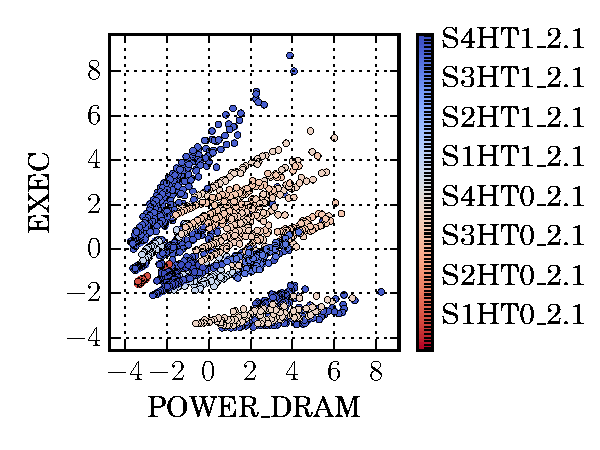
\includegraphics[width=0.3\columnwidth]{figs/classifiers/training_space_noclassifier.pdf}
\label{fig:feat-space-none}
% \vspace{ -1.5em }
}
\hspace*{0.1cm}
% \vskip -1.5em
\subfloat[SVM (Linear kernel), recall=0.456.]
{\centering 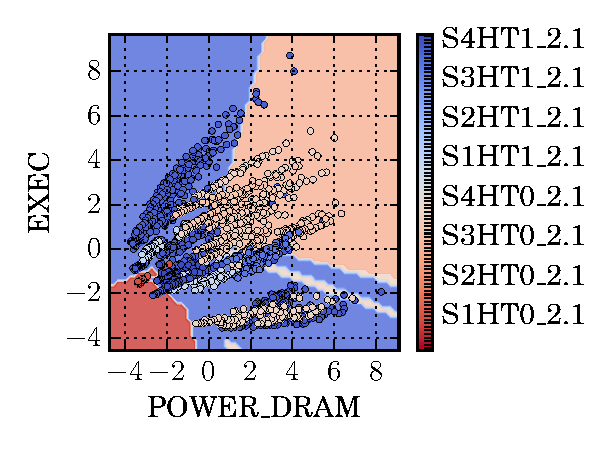
\includegraphics[width=0.3\columnwidth]{figs/classifiers/training_space_svm_kern_lin.pdf}
\label{fig:feat-space-svm-kern-lin}
% \vspace{ -1.5em }
}
\hspace*{0.1cm}
\subfloat[SVM (RBF kernel), recall=0.710.]
{\centering 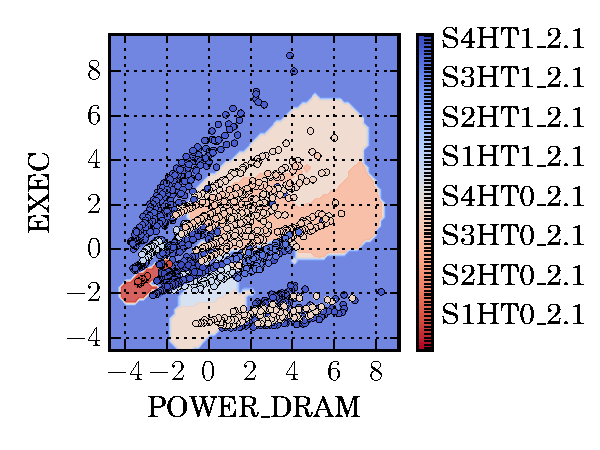
\includegraphics[width=0.3\columnwidth]{figs/classifiers/training_space_svm.pdf}
\label{fig:feat-space-svm}
% \vspace{ -1.5em }
}
\caption{Training data and learned decision boundaries for two SVM classifiers using two primary features.}
\label{fig:feat-space-intro}
% \vskip -1.0em
\end{figure}

We briefly illustrate this complexity using just two features---the performance counters \pc{POWER\_DRAM} (a measure of memory usage) and \pc{EXEC} (a measure of CPU usage).
\figref{feat-space-none} visualizes the behavior of our training data (21 common HPC benchmarks) with respect to normalized performance counter values.
Each data point is the average recorded \pc{POWER\_DRAM} and \pc{EXEC} behavior for a training application running in a single resource configuration on our evaluation system.
There are 88 unique resource configurations, or possible \emph{labels}, accounting for different combinations of the socket count \texttt{S}, whether HyperThreads \texttt{HT} are used, and the DVFS frequency (\eg 2.1\GHz).
% Thus, each application has 88 data points.
All 88 data points belonging to a particular application are assigned \emph{the same label}---the resource configuration with the best average energy efficiency for that application; \ie all 88 data points for an application have the same color.
With this labeling, a good learner will recognize suboptimal behavior and produce the most energy-efficient settings to use instead.
The problem is clearly complex---no intuitive pattern emerges that obviously maps CPU and memory usage into the most energy-efficient system settings.

To successfully map these features into accurate predictions, the learner must be able to handle this complexity, which not all learning mechanisms can.
Consider \figref{feat-space-svm-kern-lin}, which illustrates the accuracy of a Support Vector Machine (SVM) classifier using a linear kernel.
The shaded regions indicate the label (system settings) that the SVM classifier predicts for a range of feature values; the training data is overlaid for comparison.
This linear SVM's \emph{recall}---the fraction of system settings that are accurately predicted when simply replaying the training data---is only 45.6\%, a clear indication that this classifier is not effective.
In contrast, \figref{feat-space-svm} demonstrates a SVM with a radial basis function (RBF) kernel, which achieves 71.0\% recall---better, though perhaps still with room for further improvement.
Note that recall is simpler than cross-validation, since the classifier already saw the same input during supervised training.
If a classifier cannot perform accurate recall, it will likely perform even worse in deployment, when it is exposed to data it has not yet seen.

\section{Classifying System Settings}
\label{sec:classifiers-framework}

We propose to predict energy-efficient settings at runtime, without the overhead of estimating the behavior of all possible system settings before producing a result.
As with many prior works in managing power/energy in HPC systems, we use hardware performance counters to measure application and system behavior.

\begin{figure}[t]
  \begin{centering}
    \tikzset{%
  app/.style    = {draw, thin, rectangle, minimum height = 2em,
    minimum width = 2em, fill=black!25},
  block/.style    = {draw, thick, rectangle, minimum height = 2.5em,
    minimum width = 2.5em},
  blockres/.style    = {draw, thick, rectangle, minimum height = 2.5em,
    minimum width = 2.5em, fill=green!25},
  biblock/.style  = {draw, thick, rectangle, minimum height = 5.5em,
    minimum width = 6em, fill=red!25},
  sum/.style      = {draw, circle, node distance = 2cm}, % Adder
  input/.style    = {coordinate}, % Input
  output/.style   = {coordinate} % Output
}

\begin{tikzpicture}[scale=1.0,transform shape, auto, thick, node distance=1.5cm, >=triangle 45]

\draw
  % Drawing the top blocks
  % node [input, name=goalaccuracy] {} 
  % node [left of=goalaccuracy, node distance=0.35mm]{}
  % node [sum, right of=goalaccuracy] (sumaccuracy) {} % negative feedback
  node [block, align=center] (featureselection) 
    {Feature\\Selection}
  node [block, right of=featureselection, align=center, node distance=3.9cm] (classifier) 
    {Classifier}
  node [blockres, above of=classifier, align=center, node distance=1.8cm] (trainingdata) 
    {Training\\Data}
;
  % Connectng lines
% \draw[->](goalaccuracy) -- node[align=center] {Timing\\Goal}(sumaccuracy);
% \draw[->](sumaccuracy) -- node[align=center] {Timing\\Error}(featureselection);
\draw[->](featureselection) -- node[align=center] {Processed\\Data}(classifier);
\draw[->](trainingdata) -- (classifier);

% Draw software system
\draw
  node [biblock, right of=classifier, node distance=5.2cm, align=center] (system)
    {Compute\\Node\\\\}
;
\draw
  node [app, right of=classifier, node distance=5.2cm, align=center, yshift=-0.5cm] (software)
    {Application}
;

% lines from translators to software
\draw[->](classifier.east) -- node [name=ka,align=center]{System\\Settings} (classifier.east -| system.west);

% Connectng lines
\coordinate (feedbackup) at ([yshift=-0.5cm]featureselection.south);
\draw (system.west |- feedbackup) -| node [near end,align=center] {PCM\\Sample} (feedbackup);
\draw[->](feedbackup) -- node[pos=0.99] {} (featureselection);

\end{tikzpicture}
    \caption{Design for using machine learning classifiers to predict energy-efficient system settings based on performance counter behavior.}
    \label{fig:classifier-runtime}
  \end{centering}
% \vskip -1.0em
\end{figure}

\figref{classifier-runtime} demonstrates our proposed approach.
While an \textbf{application} runs on the \textbf{compute node}, hardware performance counters are polled in the background at regular intervals.
For our experiments, we use the PCM tool to collect performance counter data \cite{PCMGit}.
The \emph{PCM sample} data is scaled, then processed using Principal Component Analysis (PCA) to identify which fields correlate well with energy efficiency.
We also use \textbf{feature selection} to limit the number of hardware counters used by the classifier to reduce runtime overhead (evaluated in \secref{eval-clf-settings}).
Using this \emph{processed data}, the \textbf{classifier} predicts the most energy-efficient \emph{system settings} to use, which are then actuated on the system.
The process then repeats at the next time interval.


\subsection{Training Data}

% \TODO{Figure: Training approach as a pipeline diagram?}

A classifier must be trained before it can be used.
To collect training data, we characterize the behavior of various benchmark applications on the target platform by running them in all possible settings while collecting hardware performance counter results.
In other words, if there are $N$ different allowable settings, each application is executed $N$ times, or once in each setting.
If $M$ applications are used in training, then there are a total of $N \times M$ data points in the training set.
More precisely, each data point is a feature vector, composed of average performance counter values for an execution.

Characterization can be time-consuming, but only needs to be done once for a platform and can be completed in a reasonable period of time by keeping application execution times short.
Choosing applications that are representative of those that will be used on the system improves the likelihood that the classifier can accurately predict settings during runtime.
Additionally, training applications should be chosen that exercise the system hardware components in different patterns to cover a wide range of possible use cases.
% As with most statistical techniques, more data typically leads to better results.

Application energy efficiency (EE) is defined as the amount of work completed per unit of energy (J) used.
Low-level hardware performance counters do not have a metric for quantifying true application progress (work completed), but the instructions retired by the system (INST) is a suitable proxy.
The classifier then quantifies energy efficiency as:
\begin{eqnarray}
EE = \frac{INST}{J}
\label{eqn:ee}
\end{eqnarray}
Each application has a single most energy-efficient setting, so the $N$ executions for the $M$ training set applications are labeled with that setting:
\begin{eqnarray}
% Label = \argmax_{i \in \{1, \ldots, N\}}EE_i
Label[m][n] = \argmax_{i \in N}EE_i \,\,\,\,\,\,\forall m \in M,\,\,\forall n \in N
\label{eqn:label}
\end{eqnarray}
% A label can take any form, \eg a setting index or string name, so long as the actuator knows how to interpret it.
Ideally, total instruction count would be fixed for an application execution, then this proxy for computing energy efficiency would align with true application execution energy efficiency.
However, instruction count typically increases with the application execution time, \eg due to background processes like PCM or kernel tasks.
As such, it is important to note that labeling the most energy-efficient configuration using \eqnref{label} is different than using the minimum-energy execution from the training set.
There are two reasons for using instruction count in computing energy efficiency.
First, energy efficiency can be quantified at any point during an execution, making it a useful metric for runtime behavior analysis.
Second and more importantly, \eqnref{ee} is a function of events happening \emph{at the time}.
Total energy requires knowing all events that \emph{will} happen during the application execution, introducing the possibility that the classifiers might be learning something about application input rather than the way hardware events correspond to energy consumption.
Accounting for instructions helps to avoid this pitfall.


\subsection{Performance Counters}
\label{sec:perf-counters}

Performance counter metrics are available at different levels of granularity---system, socket, and core.
For simplicity, we limit ourselves to system-wide data.
\tblref{pcm} lists the performance counters that we process for our experiments \cite{PCMFields}.

\begin{table}[t]
\caption{Overview of system-level performance counters.}
\label{tbl:pcm}
\small
\centering
\begin{tabular}{cc}
  \textbf{Performance Counter} & \textbf{Description} \\
  \hline
  \hline
  EXEC & Instructions per nominal CPU cycle \\
  IPC & Instructions per cycle \\
  FREQ & Frequency relative to nominal CPU frequency \\
  AFREQ & FREQ, excluding the time when the CPU is sleeping \\
  L3MISS & L3 cache line misses \\
  L2MISS & L2 cache line misses \\
  L3HIT & L3 Cache hit ratio \\
  L2HIT & L2 Cache hit ratio \\
  L3MPI & L3 Cache misses per instruction \\
  L2MPI & L2 Cache misses per instruction \\
  READ & Memory read traffic \\
  WRITE & Memory write traffic \\
  INST & Number of instructions retired \\
  Proc Energy & Energy consumed by the processor \\
  DRAM Energy & Energy consumed by the DRAM \\
  \hline
  \hline
\end{tabular}
% \vskip -.7em
\end{table}

Performance counters are also translated into rates (as needed), which is necessary in order to vary the sampling interval without scaling values (evaluated in \secref{eval-clf-settings}).
Because we use PCM to collect performance counter metrics, we read more hardware counters than we process (\tblref{pcm}).
In practice, a fielded solution would reduce overhead by only reading and processing counters that are used.
Most prior works aggressively limit the hardware counters they access, both to reduce sampling overhead and to reduce computation in their models \cite{Alvarado,Curtis-Maury2008,Libutti2014}.
Additionally, using INST as a measure of application progress to compute energy efficiency is an imperfect solution.
However, prior works have used it successfully and some have even attempted to measure only those instructions considered useful in measuring application progress, \eg ignoring spinlocks or parallelization/synchronization instructions \cite{Paragon}.

\section{Experimental Design}
\label{sec:classifiers-usage}

This section describes our experimental setup, including the evaluation system, applications used for training and evaluation, and the classification algorithms tested.
We perform our evaluation on a quad-socket, 80-physical core system with 512 GB DRAM running Ubuntu Linux 14.04 LTS.
With HyperThreads, there are 160 compute threads available, \ie 20 physical and 20 virtual on each socket.
% Kernel is 4.4.0-93-generic (does not include patches for “Spectre” (CVE-2017-5753 and CVE-2017-5715) and “Meltdown” (CVE-2017-5754). which impact performance)
We use Linux kernel 4.4.0 with the intel\_pstate driver disabled so that we can use the userspace DVFS governor.


\subsection{Training Applications}
\label{sec:setup-training}


For classifier training, we characterize and label executions for a variety of parallel applications that exhibit a range of different behaviors.
Each application is configured to run with 160 threads to match the number of compute cores on the
evaluation system and to use NUMA memory interleaving.
Training applications are selected from the NAS Parallel Benchmarks \cite{NPB}, Lawrence Livermore Lab's Co-design benchmarks (AMG \cite{BoomerAMG}, Kripke \cite{Kripke}, LULESH \cite{LULESH2}, Quicksilver \cite{Quicksilver}), and Argonne's CESAR Proxy-apps (XSBench \cite{XSBench}, RSBench \cite{RSBench}).
Other applications include CoMD \cite{CoMDGit}, Berkeley's HPGMG-FV \cite{hpgmg}, a partial differential equation solver (jacobi), and STREAM \cite{stream}.
Additionally, we include a characterization of system idling behavior.
In total, there are 21 unique applications/characterizations used for training.

Each performance counter is used as a \emph{feature} for classification.
Performance counter values are converted to rates, normalized, then PCA is applied.
\figref{pca-evr} quantifies the percentage of variance contributed by the top 10 performance counters in the feature space for our system and training applications, accounting for 99\% of the total variance.
% When PCA is configured to use all the counters listed, these values sum to 1.
% \TODO{Why do POWER\_DRAM and EXEC appear twice in \figref{pca-evr}? If this is just a quirk, perhaps just show the top 10 features?}

\begin{figure}[t]
  \begin{centering}
    \begin{tikzpicture}

\begin{groupplot}[
    group style={
        group name=plots,
        group size=1 by 1,
        xlabels at=edge bottom,
        xticklabels at=edge bottom,
        vertical sep=5pt
    },
% axis x line* = bottom,
xlabel near ticks,
major x tick style = transparent,
xlabel={},
height=3.5cm,
width=0.95\columnwidth,
xmin=0.5,
% xmax=16.5,
xmax=10.5,
enlargelimits=false,
tick align = outside,
tick style={white},
ytick=\empty,
xticklabel shift={0pt},
x tick label style={rotate=35, anchor=east, font=\scriptsize},
xtick={1,2,3,4,5,6,7,8,9,10,11,12,13,14,15,16},
xticklabels={{POWER\_DRAM},
{EXEC},
{L3HIT},
{AFREQ},
{FREQ},
{L3MPI},
{L2HIT},
{L3HIT},
{FREQ},
{POWER\_Proc},
% {WRITE\_Rate},
% {L2MPI},
% {L3MISS\_Rate},
% {POWER\_DRAM},
% {EXEC},
% {POWER\_Total}
},
ymin=0,
ymax=.5,
ytick={0,0.1,0.2,0.3,0.4,0.5},
yticklabels={0.0,0.1,0.2,0.3,0.4,0.5},
legend cell align=left, 
legend style={ column sep=1ex },
ymajorgrids,
grid style={dashed},
ylabel={\footnotesize PCA Variance},
ylabel shift={0mm},
]
\nextgroupplot[ybar=\pgflinewidth,
bar width=8pt,
]
\addplot table[x index=0,y index=2, col sep=tab] {img/classifiers/pca_evr.txt};


\end{groupplot}

\end{tikzpicture}

    \caption{PCA Explained Variance Ratio for the top 10 performance counters, accounting for 99\% of variance.}
    \label{fig:pca-evr}
  \end{centering}
% \vskip -1.0em
\end{figure}


\subsection{Evaluation Applications}
\label{sec:setup-evaluation}

We evaluate classifier performance on four complex bioinformatic HPC applications: HipMer~\cite{georganas2015hipmer}, IDBA~\cite{peng2012idba}, Megahit~\cite{li2015megahit} and metaSPAdes~\cite{nurk2016metaspades}.
These four are the leading applications that perform \emph{de novo} genome assembly, which is one of the most computationally challenging bioinformatics problems.
The datasets can be very large (for example, metagenomes can have raw sequence datasets on the order of terabytes), and the algorithms are hard to scale efficiently.
For example, of the four applications, only HipMer scales efficiently to distributed memory systems.
Consequently, \emph{de novo} assemblers are typically run on very large shared-memory systems, with at least 0.5TB of memory.
Thus our experimental platform is typical of the sort of hardware that would be used for these kinds of applications.

Furthermore, these applications implement complex pipelines, with multiple different stages, some of which are compute-intensive, some I/O-intensive, and some communication-intensive.
Exactly which stages are used and how much they contribute to the performance depends to a large degree on the program configuration and the input datasets.
A single execution assembling a large genome could take days on our large evaluation system, making it prohibitive to exhaustively characterize the full range of allowable settings.
Even running a partial characterization (like DVFS-only) for a fixed input is unrealistic for most such applications in practice, motivating the need for a general solution.

Although these four applications are solving the same problem, they are implemented in very different ways, with different programming languages, different algorithms and different data flows.
For example, HipMer can have up to 20 different stages, whereas Megahit may have only a few.
Overall, these applications provide a broad coverage of a range of different bioinformatics approaches (frequency counting, graph traversal, alignment, sorting, etc.).

Like with training applications, we configure each evaluation application to run with 160 threads, except for metaSPAdes which uses 80 threads.
We fix the application inputs and configurations for our evaluation, but of course they support a variety of configurations and inputs which affect performance and energy consumption behavior.
% Due to the long application runtimes, it is infeasible to characterize these applications in all configurations, despite the application settings and inputs being fixed.
Solely to use as a baseline in our evaluation, we perform a time-consuming DVFS-only characterization by running them in each DVFS setting with all 160 virtual cores allocated (for metaSPAdes, all 80 physical cores are used as the baseline instead).
Note that this data is \emph{not} used in classifier training.
Based on these partial characterizations, we see that \emph{each application has a different most energy-efficient static setting}.
The applications are thus prime candidates for our approach of using classification to predict the appropriate settings at runtime.


\subsection{Classification Algorithms}

This section identifies and briefly describes the classifiers we use.
For data processing and classifier implementations, we use the Machine Learning toolkit scikit-learn, version 0.19.1 \cite{scikit-learn}.
% See the scikit-learn documentation for implementation details.
We do not attempt to optimize algorithm performance or prediction accuracy by tuning any implementation knobs.
We demonstrate the feasibility of using classification without the need for fine-tuning.

\begin{figure}[t]
  \begin{centering}
    \begin{tikzpicture}

\begin{groupplot}[
    group style={
        group name=plots,
        group size=1 by 1,
        xlabels at=edge bottom,
        xticklabels at=edge bottom,
        vertical sep=5pt
    },
% axis x line* = bottom,
xlabel near ticks,
major x tick style = transparent,
xlabel={},
height=3.5cm,
width=0.95\columnwidth,
xmin=0.5,
% xmax=16.5,
xmax=15.5,
enlargelimits=false,
tick align = outside,
tick style={white},
ytick=\empty,
xticklabel shift={0pt},
x tick label style={rotate=35, anchor=east, font=\scriptsize},
xtick={1,2,3,4,5,6,7,8,9,10,11,12,13,14,15,16},
xticklabels={
% {AdaBoost},
% {Decision~Tree},
% {Extra~Trees},
% {Gradient~Boosting},
% {Gaussian~Naive~Bayes},
% {K-Nearest~Neighbor},
% {Linear~Discriminant~Analysis},
% {MultiLayer~Perceptron},
% {Quadratic~Discriminant~Analysis},
% {Random~Forest},
% {Stochastic~Gradient~Descent},
% {SVM~Linear~Kernel},
% {SVM~Polynomial~Kernel},
% {SVMLinear},
% {SVM~RBF~Kernel},
{AB},
{DT},
{ET},
{GB},
{GNB},
{KNN},
{LDA},
{MLP},
{QDA},
{RF},
{SGD},
{SVM~(Lin)},
{SVM~(Poly3)},
{SVMLinear},
{SVM~(RBF)},
},
ymin=0,
ymax=1.1,
ytick={0,0.2,0.4,0.6,0.8,1.0},
yticklabels={0,0.2,0.4,0.6,0.8,1.0},
legend cell align=left, 
legend style={ column sep=1ex },
ymajorgrids,
grid style={dashed},
ylabel={\footnotesize Training Recall},
ylabel shift={0mm},
]
\nextgroupplot[ybar=\pgflinewidth,
bar width=8pt,
]
\addplot table[x index=0,y index=2, col sep=tab] {img/classifiers/classifier_recall.txt};


\end{groupplot}

\end{tikzpicture}

    \caption{Training data recall for 15 classification algorithm implementations.}
    \label{fig:recall}
  \end{centering}
% \vskip -1.0em
\end{figure}

With the labeled training data in \figref{feat-space-none} (\secref{challenges-learning}), it is clear that the a useful classification algorithm must handle a complex space.
We validate this hypothesis by performing an offline analysis of $15$ algorithms using our training data.
One of the metrics we looked at was training data recall, which we present in \figref{recall}.
The algorithms are: AdaBoost (AB), Decision Tree (DT), Extra Trees (ET), Gradient Boosting (GB), Gaussian Naive Bayes (GNB), K-Nearest Neighbors (KNN), Linear Discriminant Analysis (LDA), Multi-layer Perceptron (MLP), Quadratic Discriminant Analysis (QDA), Random Forest (RF), Stochastic Gradient Descent (SGD), Support Vector Machine with a linear kernel (SVM (Lin)), SVM with a degree=3 polynomial kernel (SVM (Poly3)), SVM with a different linear kernel (SVMLinear), and SVM with a radial basis function kernel (SVM (RBF)).
Some approaches have poor recall and thus are not likely to perform well in practice.

When a mis-prediction occurs, the impact on energy consumption varies---some are suboptimal but still reduce energy consumption over the naive \emph{race-to-idle} heuristic, while others actually make it worse.
We tested SVM (Lin) (\figref{feat-space-svm-kern-lin}) online---in most cases it reduced energy, but consumed 22\% \emph{more energy} than \emph{race-to-idle} with the Megahit application, demonstrating the importance of selecting a good classifier.
We choose five promising algorithms that support a range of different classification techniques to use in the evaluation:
\begin{enumerate}
\item ET -- an extremely randomized decision tree, similar to Random Forest \cite{Geurts2006ExtraTrees}.
\item GB -- fits multiple regression trees on the negative gradient of the deviance loss function \cite{scikit-learn, friedman2001GradientBoosting}.% cites scikit-learn for the definition
\item KNN -- a simple majority vote of the nearest neighbors from the training data ($k=5$, by default).
\item MLP -- a neural network optimizing the log-loss function using \emph{lbfgs}, a \emph{tanh} activation function, and four layers \cite{HintonMultiLayerPerceptron}.
\item SVM -- a maximum margin classifier using a radial basis function (RBF) kernel.
\end{enumerate}
The only classifier with non-default configurations is MLP, in order to add additional layers to better represent deep learners, and to specify the activation and solver functions.
Our evaluation compares the energy consumption of real application executions when using these five classifiers in different configurations.

\section{Evaluation}
\label{sec:classifiers-evaluation}

We now evaluate the effectiveness of using machine learning classifiers to predict energy-efficient system settings during application runtime.
First, we compare against the naive \emph{race-to-idle} heuristic, \ie all sockets allocated with HyperThreads and DVFS set to TurboBoost, and against a DVFS \emph{Oracle}.
We then quantify how varying sampling/prediction intervals and the number and types of features impacts classifier effectiveness.
We discuss how application dynamics affect the classifiers and evaluate the overhead of different parts of the classifier runtime.
Finally, we explore using separate classifiers for taskset and DVFS, then discuss limitations.


\subsection{Reducing Energy Consumption}
\label{sec:eval-first}

\begin{figure}[t]
  \centering
  \begin{tikzpicture}
\definecolor{s1}{RGB}{228, 26, 28}
\definecolor{s2}{RGB}{55, 126, 184}
\definecolor{s3}{RGB}{77, 175, 74}
\definecolor{s4}{RGB}{152, 78, 163}
\definecolor{s5}{RGB}{255, 127, 0}

\begin{groupplot}[
    group style={
        group name=plots,
        group size=1 by 1,
        xlabels at=edge bottom,
        xticklabels at=edge bottom,
        vertical sep=5pt
    },
% axis x line* = bottom,
xlabel near ticks,
major x tick style = transparent,
xlabel={},
height=3.5cm,
width=0.95\columnwidth,
xmin=0.5,
xmax=4.5,
enlargelimits=false,
tick align = outside,
tick style={white},
ylabel style={align=center},
ytick=\empty,
ymin=0.6,
ymax=1.1,
ytick={0,0.2,0.4,0.6,0.8,1.0,1.2},
yticklabels={0.0,0.2,0.4,0.6,0.8,1.0,1.2},
legend cell align=left, 
legend style={ column sep=1ex },
ymajorgrids,
grid style={dashed},
]

\nextgroupplot[ylabel={Energy \\ (Normalized)},
ybar=\pgflinewidth,
legend entries = {{ET},{GB},{KNN},{MLP},{SVM},{Oracle}},
legend style={draw=none,legend columns=6,at={(.5,1.4)},anchor=north},
bar width=8pt,
ylabel shift={0mm},
xticklabel shift={0pt},
x tick label style={rotate=35, anchor=east, font=\scriptsize},
xtick={1,2,3,4,5,6,7},
xticklabels={
{HipMer},
{IDBA},
{Megahit},
{metaSPAdes},
},
execute at end plot={
% "Race":
\draw[thin, dashed] (axis cs:\pgfkeysvalueof{/pgfplots/xmin},1) -- (axis cs:\pgfkeysvalueof{/pgfplots/xmax},1);
% "Best static DVFS":
% \draw[thick, dotted] (axis cs:\pgfkeysvalueof{/pgfplots/xmin},0.765646972) -- (axis cs:\pgfkeysvalueof{/pgfplots/xmax},0.765646972);
% hack to reset column line style (ghostscript seems to use last formatting as line style, e.g. dashed or dotted instead of solid)
\draw[thin, solid] (axis cs:\pgfkeysvalueof{/pgfplots/xmin},\pgfkeysvalueof{/pgfplots/ymin}) -- (axis cs:\pgfkeysvalueof{/pgfplots/xmax},\pgfkeysvalueof{/pgfplots/ymin});
},
]
\addplot table[x index=0,y index=2, col sep=tab] {img/classifiers/compare_apps_pca4.txt};
\addplot table[x index=0,y index=3, col sep=tab] {img/classifiers/compare_apps_pca4.txt};
\addplot table[x index=0,y index=4, col sep=tab] {img/classifiers/compare_apps_pca4.txt};
\addplot table[x index=0,y index=5, col sep=tab] {img/classifiers/compare_apps_pca4.txt};
\addplot table[x index=0,y index=6, col sep=tab] {img/classifiers/compare_apps_pca4.txt};
\addplot table[x index=0,y index=7, col sep=tab] {img/classifiers/compare_apps_pca4.txt};

\end{groupplot}

\end{tikzpicture}
  \caption{Average application energy consumption using four performance counters at 5 second prediction intervals (lower is better).}
  \label{fig:compare-apps-pca4}
  % \vskip -1.0em
\end{figure}

We first demonstrate how effective runtime classification is at reducing energy consumption.
\figref{compare-apps-pca4} demonstrates results for each application, normalized to the \emph{race-to-idle} setting (dashed line) for each.
On average across all four applications, energy consumption is reduced by 19.3\%.
The most extreme results are from the \app{IDBA} and \app{Megahit} applications.
For \app{IDBA}, each classifier outperforms the \emph{Oracle}---the average energy savings is 28.1\%, and as much as 30.2\% when using the GB classifier.
Conversely, for \app{Megahit}, the classifiers have the highest energy consumption over the \emph{Oracle}, though still always better than \emph{race-to-idle}.
\app{Megahit} saves 11\% energy on average---8.7\% in the worst case with ET, and 15\% at best with MLP.
The behavior for these applications is discussed further in \secref{eval-dynamics}.
% We note both here and in the remainder of the evaluation that there is no consistently best classifier across applications.

The \emph{Oracle} is the most energy-efficient statically-selected DVFS frequency using all sockets and HyperThreads, and it difficult to beat.
Computing the \emph{Oracle} requires expensive offline characterization to determine the best static setting for each application and its input/configuration, making it impractical to determine for most applications.
It also does not have any overhead except for running PCM in the background.
The \emph{Oracle} can only be beat when an application does not require its full taskset (socket and HyperThreads) allocation to run efficiently.
HPC applications are designed to parallelize well, meaning this is not the typical use case, but opportunities do occur, \eg during prolonged memory or I/O-intensive phases.

\begin{figure}[t]
% python ClassificationPlotUtils.py -s boggle -c boggle/characterizations/HIPMER/0xFFFFFFFFFFFFFFFFFFFFFFFFFFFFFFFFFFFFFFFF_2101000/pcm.csv boggle/classifications/5s/HIPMER_moredata/ET/pcm.csv -i 1 5
  \centering
  % \vskip -0.1em
  \subfloat[\app{HipMer} in naive static \emph{race-to-idle} heuristic.]
  % {\centering \includegraphics[width=\columnwidth]{figs/ts_hipmer_2101000_pca4.pdf}
  {\centering \begin{tikzpicture}

\definecolor{s1}{RGB}{228, 26, 28}
\definecolor{s2}{RGB}{55, 126, 184}
\definecolor{s3}{RGB}{77, 175, 74}
\definecolor{s4}{RGB}{152, 78, 163}
\definecolor{s5}{RGB}{255, 127, 0}

\begin{groupplot}[
    group style={
        group name=plots,
        group size=1 by 1,
        xlabels at=edge bottom,
        xticklabels at=edge bottom,
        vertical sep=5pt
    },
height=3.5cm,
width=0.95\columnwidth,
xmajorgrids,
ymajorgrids,
grid style={dashed},
xmin=0,
xmax=3465,
xtick={0,500,1000,1500,2000,2500,3000,3500},
ymin=0,
ymax=1.05,
ytick={0,0.2,0.4,0.6,0.8,1.0},
yticklabels={0,0.2,0.4,0.6,0.8,1.0},
yticklabel pos=left,
enlargelimits=false,
tick align = outside,
tick style={white},
xticklabel shift={-5pt},
yticklabel shift={-5pt},
ylabel shift={-2pt},
ylabel style={align=center},
legend cell align=left,
legend style={ column sep=1ex },
unbounded coords=jump,
]

\nextgroupplot[ylabel={},
yticklabel style={font=\footnotesize},
xlabel={\footnotesize $time$ [seconds]},
xlabel near ticks,
xticklabels={0,500,1000,1500,2000,2500,3000,3500},
xticklabel style={font=\footnotesize},
legend entries={{Power},{EE},{Cumulative~Energy}},
legend style={draw=none,at={(0.5,1.4)},anchor=north,legend columns=4,line width=5pt},
]
\addplot[thick, solid, color=s2] table[x index=0,y index=1,col sep=comma] {img/classifiers/ts_hipmer/ts_hipmer_2101000_pca4.csv};
\addplot[thick, solid, color=s3] table[x index=0,y index=2,col sep=comma] {img/classifiers/ts_hipmer/ts_hipmer_2101000_pca4.csv};
\addplot[thick, solid, color=s1] table[x index=0,y index=3,col sep=comma] {img/classifiers/ts_hipmer/ts_hipmer_2101000_pca4.csv};
\addplot[thin, solid, black] coordinates {(2206,0) (2206, 250)};

\end{groupplot}

\end{tikzpicture}
  \label{fig:ts-hipmer-dvfs}
  % \vspace{ -1.5em }
  }
  \\
  % \vskip -1.5em
  \subfloat[\app{HipMer} with ET classifier at 5 second intervals.]
  % {\centering \includegraphics[width=\columnwidth]{figs/ts_hipmer_et_pca4.pdf}
  {\centering \begin{tikzpicture}

\definecolor{s1}{RGB}{228, 26, 28}
\definecolor{s2}{RGB}{55, 126, 184}
\definecolor{s3}{RGB}{77, 175, 74}
\definecolor{s4}{RGB}{152, 78, 163}
\definecolor{s5}{RGB}{255, 127, 0}

\begin{groupplot}[
    group style={
        group name=plots,
        group size=1 by 1,
        xlabels at=edge bottom,
        xticklabels at=edge bottom,
        vertical sep=5pt
    },
height=3.5cm,
width=0.95\columnwidth,
xmajorgrids,
ymajorgrids,
grid style={dashed},
xmin=0,
xmax=3465,
xtick={0,500,1000,1500,2000,2500,3000,3500},
ymin=0,
ymax=1.05,
ytick={0,0.2,0.4,0.6,0.8,1.0},
yticklabels={0,0.2,0.4,0.6,0.8,1.0},
yticklabel pos=left,
enlargelimits=false,
tick align = outside,
tick style={white},
xticklabel shift={-5pt},
yticklabel shift={-5pt},
ylabel shift={-2pt},
ylabel style={align=center},
legend cell align=left,
legend style={ column sep=1ex },
unbounded coords=jump,
]

\nextgroupplot[ylabel={},
yticklabel style={font=\footnotesize},
xlabel={\footnotesize $time$ [seconds]},
xlabel near ticks,
xticklabels={0,500,1000,1500,2000,2500,3000,3500},
xticklabel style={font=\footnotesize},
legend entries={{Power},{EE},{Cumulative.~Energy}},
legend style={draw=none,at={(0.5,1.4)},anchor=north,legend columns=4,line width=5pt},
]
\addplot[thick, solid, color=s2] table[x index=0,y index=1,col sep=comma] {img/classifiers/ts_hipmer/ts_hipmer_et_pca4.csv};
\addplot[thick, solid, color=s3] table[x index=0,y index=2,col sep=comma] {img/classifiers/ts_hipmer/ts_hipmer_et_pca4.csv};
\addplot[thick, solid, color=s1] table[x index=0,y index=3,col sep=comma] {img/classifiers/ts_hipmer/ts_hipmer_et_pca4.csv};
\addplot[thin, solid, black] coordinates {(3465,0) (3465, 250)};

\end{groupplot}

\end{tikzpicture}
  \label{fig:ts-hipmer-all-et}
  % \vspace{ -1.5em }
  }
  \caption{Execution time, power, energy efficiency, and energy consumption behavior for the \app{HipMer} application (a) without and (b) with classification.}
  \label{fig:ts-hipmer}
  % \vskip -1.0em
\end{figure}

To demonstrate how energy savings are achieved, \figref{ts-hipmer} shows the runtime, power, energy efficiency, and cumulative energy consumption for executions of the \app{HipMer} application (Y values are normalized across both time series for each metric).
\figref{ts-hipmer-dvfs} runs \app{HipMer} in the \emph{race-to-idle} heuristic, and although the runtime is short, the high power also results in poor energy consumption.
In contrast, \figref{ts-hipmer-all-et} demonstrates running with the ET classifier---the execution takes longer, but the significantly lower power results in nearly 20\% less energy consumption in total, despite the increase in runtime.
Each figure shows clear phases in the execution, indicated by relatively long-term changes in both power and energy efficiency (per \eqnref{ee}, a function of instruction rate and power).
Classifiers adapt to changes in feature values like instruction rate and power by changing their predictions to run the application more efficiently, thus decreasing total energy consumption.


\subsection{Classifier Interval and Feature Selection}
\label{sec:eval-clf-settings}

\begin{figure}[t]
  \centering
  \begin{tikzpicture}
\definecolor{s1}{RGB}{228, 26, 28}
\definecolor{s2}{RGB}{55, 126, 184}
\definecolor{s3}{RGB}{77, 175, 74}
\definecolor{s4}{RGB}{152, 78, 163}
\definecolor{s5}{RGB}{255, 127, 0}

\begin{groupplot}[
    group style={
        group name=plots,
        group size=1 by 1,
        xlabels at=edge bottom,
        xticklabels at=edge bottom,
        vertical sep=5pt
    },
% axis x line* = bottom,
xlabel near ticks,
major x tick style = transparent,
xlabel={},
height=3.5cm,
width=0.95\columnwidth,
xmin=0.5,
xmax=5.5,
enlargelimits=false,
tick align = outside,
tick style={white},
ylabel style={align=center},
ytick=\empty,
ymin=0.6,
ymax=1.1,
ytick={0.6,0.7,0.8,0.9,1.0,1.1},
yticklabels={0.6,0.7,0.8,0.9,1.0,1.1},
legend cell align=left, 
legend style={ column sep=1ex },
ymajorgrids,
grid style={dashed},
]

\nextgroupplot[ylabel={Energy \\ (Normalized)},
ybar=\pgflinewidth,
legend entries = {{1~sec},{5~sec},{10~sec}},
legend style={draw=none,legend columns=5,at={(.5,1.4)},anchor=north},
bar width=8pt,
ylabel shift={0mm},
xticklabel shift={0pt},
x tick label style={rotate=35, anchor=east, font=\scriptsize},
xtick={1,2,3,4,5,6,7},
xticklabels={
{ET},
{GB},
{KNN},
{MLP},
{SVM},
},
execute at end plot={
% "Race":
\draw[thin, dashed] (axis cs:\pgfkeysvalueof{/pgfplots/xmin},1) -- (axis cs:\pgfkeysvalueof{/pgfplots/xmax},1);
% "Best static DVFS":
\draw[thick, dotted] (axis cs:\pgfkeysvalueof{/pgfplots/xmin},0.765646972) -- (axis cs:\pgfkeysvalueof{/pgfplots/xmax},0.765646972);
% hack to reset column line style (ghostscript seems to use last formatting as line style, e.g. dashed or dotted instead of solid)
\draw[thin, solid] (axis cs:\pgfkeysvalueof{/pgfplots/xmin},\pgfkeysvalueof{/pgfplots/ymin}) -- (axis cs:\pgfkeysvalueof{/pgfplots/xmax},\pgfkeysvalueof{/pgfplots/ymin});
},
]
\addplot table[x index=0,y index=7, col sep=tab] {img/classifiers/compare_interval/compare_1s.txt};
\addplot table[x index=0,y index=7, col sep=tab] {img/classifiers/compare_interval/compare_5s.txt};
\addplot table[x index=0,y index=7, col sep=tab] {img/classifiers/compare_interval/compare_10s.txt};

\end{groupplot}

\end{tikzpicture}
  \caption{Average energy consumption for different sampling/prediction intervals (lower is better).}
  \label{fig:interval}
  % \vskip -1.0em
\end{figure}

There are a variety classifier settings to configure at runtime.
This section evaluates the classifiers' ability to reduce energy consumption by varying prediction interval and the number and types of features used.

The sampling and prediction interval dictates how quickly a classifier can respond to changes in application behavior, but also incurs overhead and affects a classifier's susceptibility to noise.
\figref{interval} shows the normalized energy consumption, averaged across applications, for each classifier at 1, 5, and 10 second intervals.
The thin dotted line at 0.75 is the average normalized energy consumption for the \emph{Oracle}.
The 1 second interval is clearly the worst, only outperforming the others for the ET classifier.
It is closer to the \emph{race-to-idle} heuristic than the \emph{Oracle} for GB and SVM, but still better than \emph{race-to-idle}.
Both the 5 and 10 second intervals perform well---although the 10 second interval does better for one particular classifier (KNN), the 5 second interval is similar on average and is more responsive.
We elect to use the 5 second interval for the remainder of our experiments, as it provides a good tradeoff of energy efficiency and responsiveness to changing application behavior.

\begin{figure}[t]
  \centering
  % \vskip -0.1em
  \subfloat[Average energy consumption based on number of features.]
  {\centering \begin{tikzpicture}
\definecolor{s1}{RGB}{228, 26, 28}
\definecolor{s2}{RGB}{55, 126, 184}
\definecolor{s3}{RGB}{77, 175, 74}
\definecolor{s4}{RGB}{152, 78, 163}
\definecolor{s5}{RGB}{255, 127, 0}

\begin{groupplot}[
    group style={
        group name=plots,
        group size=1 by 1,
        xlabels at=edge bottom,
        xticklabels at=edge bottom,
        vertical sep=5pt
    },
% axis x line* = bottom,
xlabel near ticks,
major x tick style = transparent,
xlabel={},
height=3.5cm,
width=0.95\columnwidth,
xmin=0.5,
xmax=5.5,
enlargelimits=false,
tick align = outside,
tick style={white},
ylabel style={align=center},
ytick=\empty,
ymin=0.6,
ymax=1.1,
ytick={0.6,0.7,0.8,0.9,1.0,1.1},
yticklabels={0.6,0.7,0.8,0.9,1.0,1.1},
legend cell align=left, 
legend style={ column sep=1ex },
ymajorgrids,
grid style={dashed},
]

\nextgroupplot[ylabel={Energy \\ (Normalized)},
ybar=\pgflinewidth,
legend entries = {{One},{Two},{Three},{Four},{Five},{All}},
legend style={draw=none,legend columns=6,at={(.5,1.4)},anchor=north},
bar width=8pt,
ylabel shift={0mm},
xticklabel shift={0pt},
x tick label style={rotate=35, anchor=east, font=\scriptsize},
xtick={1,2,3,4,5,6,7},
xticklabels={
{ET},
{GB},
{KNN},
{MLP},
{SVM},
},
execute at end plot={
% "Race":
\draw[thin, dashed] (axis cs:\pgfkeysvalueof{/pgfplots/xmin},1) -- (axis cs:\pgfkeysvalueof{/pgfplots/xmax},1);
% "Best static DVFS":
\draw[thick, dotted] (axis cs:\pgfkeysvalueof{/pgfplots/xmin},0.765646972) -- (axis cs:\pgfkeysvalueof{/pgfplots/xmax},0.765646972);
% hack to reset column line style (ghostscript seems to use last formatting as line style, e.g. dashed or dotted instead of solid)
\draw[thin, solid] (axis cs:\pgfkeysvalueof{/pgfplots/xmin},\pgfkeysvalueof{/pgfplots/ymin}) -- (axis cs:\pgfkeysvalueof{/pgfplots/xmax},\pgfkeysvalueof{/pgfplots/ymin});
},
]
\addplot table[x index=0,y index=7, col sep=tab] {img/classifiers/compare_pca/pca1.txt};
\addplot table[x index=0,y index=7, col sep=tab] {img/classifiers/compare_pca/pca2.txt};
\addplot table[x index=0,y index=7, col sep=tab] {img/classifiers/compare_pca/pca3.txt};
\addplot table[x index=0,y index=7, col sep=tab] {img/classifiers/compare_pca/pca4.txt};
\addplot table[x index=0,y index=7, col sep=tab] {img/classifiers/compare_pca/pca5.txt};
\addplot table[x index=0,y index=7, col sep=tab] {img/classifiers/compare_interval/compare_5s.txt};

\end{groupplot}

\end{tikzpicture}
  \label{fig:compare-pca}
  % \vspace{ -1.5em }
  }
  \\
  % \vskip -1.5em
  \subfloat[Average energy consumption based on types of features.]
  {\centering \begin{tikzpicture}
\definecolor{s1}{RGB}{228, 26, 28}
\definecolor{s2}{RGB}{55, 126, 184}
\definecolor{s3}{RGB}{77, 175, 74}
\definecolor{s4}{RGB}{152, 78, 163}
\definecolor{s5}{RGB}{255, 127, 0}

\begin{groupplot}[
    group style={
        group name=plots,
        group size=1 by 1,
        xlabels at=edge bottom,
        xticklabels at=edge bottom,
        vertical sep=5pt
    },
% axis x line* = bottom,
xlabel near ticks,
major x tick style = transparent,
xlabel={},
height=3.5cm,
width=0.95\columnwidth,
xmin=0.5,
xmax=5.5,
enlargelimits=false,
tick align = outside,
tick style={white},
ylabel style={align=center},
ytick=\empty,
ymin=0.6,
ymax=1.1,
ytick={0,0.2,0.4,0.6,0.8,1.0,1.2},
yticklabels={0.0,0.2,0.4,0.6,0.8,1.0,1.2},
legend cell align=left, 
legend style={ column sep=1ex },
ymajorgrids,
grid style={dashed},
]

\nextgroupplot[ylabel={Energy \\ (Normalized)},
ybar=\pgflinewidth,
legend entries = {{All},{NoPower},{NoDramTotalExec}},
legend style={draw=none,legend columns=4,at={(.5,1.4)},anchor=north},
bar width=8pt,
ylabel shift={0mm},
xticklabel shift={0pt},
x tick label style={rotate=35, anchor=east, font=\scriptsize},
xtick={1,2,3,4,5,6,7},
xticklabels={
{ET},
{GB},
{KNN},
{MLP},
{SVM},
},
execute at end plot={
% "Race":
\draw[thin, dashed] (axis cs:\pgfkeysvalueof{/pgfplots/xmin},1) -- (axis cs:\pgfkeysvalueof{/pgfplots/xmax},1);
% "Best static DVFS":
\draw[thick, dotted] (axis cs:\pgfkeysvalueof{/pgfplots/xmin},0.765646972) -- (axis cs:\pgfkeysvalueof{/pgfplots/xmax},0.765646972);
% hack to reset column line style (ghostscript seems to use last formatting as line style, e.g. dashed or dotted instead of solid)
\draw[thin, solid] (axis cs:\pgfkeysvalueof{/pgfplots/xmin},\pgfkeysvalueof{/pgfplots/ymin}) -- (axis cs:\pgfkeysvalueof{/pgfplots/xmax},\pgfkeysvalueof{/pgfplots/ymin});
},
]

\addplot table[x index=0,y index=7, col sep=tab] {img/classifiers/compare_interval/compare_5s.txt};
\addplot table[x index=0,y index=7, col sep=tab] {img/classifiers/compare_pca/pca_nopower.txt};
\addplot table[x index=0,y index=7, col sep=tab] {img/classifiers/compare_pca/pca_nodramtotalexec.txt};

\end{groupplot}

\end{tikzpicture}
  \label{fig:compare-robustness}
  % \vspace{ -1.5em }
}
  \caption{Average energy consumption, varying the number and types of available features (lower is better).}
  \label{fig:pca}
  % \vskip -1.0em
\end{figure}

In \figref{pca-evr} (\secref{setup-training}) we quantified the variation contribution of different features (performance counters).
Now we evaluate how varying the features impacts classifier behavior, since the number and types of features contribute to runtime complexity and prediction accuracy.
We run with 5 second sampling/prediction intervals and present the results in \figref{pca}.

\figref{compare-pca} varies the number of features used.
\pc{POWER\_DRAM} is the only feature used for $One$, \pc{POWER\_DRAM} and \pc{EXEC} are used for $Two$, etc.
For $All$, all 16 features are used.
Using a single feature works surprisingly well for most classifiers, but performs poorly with KNN, which too often predicts settings that use only a single socket.
It is a little surprising that a single feature can be so effective otherwise, but \pc{POWER\_DRAM} does account for 42\% of the explained variance, and is correlated with other performance counters like cache hit and miss rates.
Using two or three features also works quite well, but four features is the best for most classifiers, accounting for 84\% of the variance.
The $Four$ configuration was previously broken down by application in \secref{eval-first}.

\figref{compare-robustness} selectively removes available features.
$NoPower$ drops the \pc{POWER\_DRAM}, \pc{POWER\_Proc}, and \pc{POWER\_Total} features.
This is a particularly important scenario, as not all systems have power/energy counters available at runtime.
When all three power-related features are ignored, \pc{L3MISS\_Rate} is used as the first feature, and \pc{EXEC} remains the second.
(If \pc{POWER\_DRAM} is excluded exclusively, \pc{POWER\_Total} becomes the primary feature instead.)
Offline analysis also shows that \pc{READ\_Rate} can be used as the primary feature, depending on the exact training data.
$NoDramTotalExec$ drops \pc{POWER\_DRAM}, \pc{POWER\_Total}, and \pc{EXEC}, making \pc{AFREQ} and \pc{WRITE\_Rate} the primary and secondary features.
In general, $All$ outperforms the other two, but $NoPower$ does slightly better for the ET classifier, as does $NoDramTotalExec$ with MLP.
None of the configurations perform poorly, demonstrating that the classification approach is robust to different numbers and types of features.


\subsection{Application Dynamics}
\label{sec:eval-dynamics}

The results thus far raise the question: why does the \emph{Oracle} often perform better than the classifiers?
First, we recall that the \emph{Oracle} requires each application to be characterized across all DVFS settings with their current input and configuration, so is not practical to discover for most applications in practice.
Additionally, the \emph{Oracle} does not incur any overhead except sampling PCM (runtime overheads are quantified next in \secref{classifiers-eval-overhead}), and can only be beat when applications do not require all sockets and HyperThreads.
In fact, for 3 of the 4 evaluation applications, classification usually achieves energy consumption close to that of the \emph{Oracle}, and sometimes better.

Energy consumption penalties are incurred primarily by two factors: (1) overhead from changing settings, and (2) running in inefficient settings.
While there is no particular threshold for determining when changes to performance counter values result in a new prediction, we quantify the difficulty in controlling applications by examining performance counters' coefficients of variation during the course of an application execution.
Since applications move through phases, a high coefficient of variation for an execution does not cause problems on its own.
The difficulty arises when performance counter values fluctuate rapidly enough to cause the classifiers to predict new system settings, constantly incurring actuation overhead and spending time in suboptimal settings.

\begin{figure}[t]
  \centering
  \begin{tikzpicture}

\definecolor{s1}{RGB}{228, 26, 28}
\definecolor{s2}{RGB}{55, 126, 184}
\definecolor{s3}{RGB}{77, 175, 74}
\definecolor{s4}{RGB}{152, 78, 163}
\definecolor{s5}{RGB}{255, 127, 0}

\begin{groupplot}[
    group style={
        group name=plots,
        group size=1 by 2,
        xlabels at=edge bottom,
        xticklabels at=edge bottom,
        vertical sep=5pt
    },
height=3.5cm,
width=\columnwidth,
xmajorgrids,
ymajorgrids,
grid style={dashed},
xmin=0,
xmax=600,
yticklabel pos=left,
enlargelimits=false,
tick align = outside,
tick style={white},
xticklabel shift={-5pt},
yticklabel shift={-5pt},
ylabel shift={-2pt},
ylabel style={align=center},
legend cell align=left,
legend style={ column sep=1ex },
unbounded coords=jump,
]

\nextgroupplot[ylabel={IDBA \\ Coeff. of Var.},
ytick={0,0.5,1.0,1.5,2.0},
yticklabels={,0.5,1.0,1.5,2.0},
yticklabel style={font=\footnotesize},
ymin=0,
ymax=2,
% xlabel={\footnotesize Time (s)},
xlabel near ticks,
xtick={0,100,200,300,400,500,600},
% xticklabels={0,100,200,300,400,500,600},
xticklabel style={font=\footnotesize},
legend entries={{POWER\_DRAM},{EXEC}},
legend style={draw=none,at={(0.5,1.4)},anchor=north,legend columns=4,line width=5pt},
]
\addplot[thick, solid, color=s1] table[x index=0,y index=2,col sep=tab] {img/classifiers/cv/coev_idba.txt};
\addplot[thick, solid, color=s2] table[x index=0,y index=1,col sep=tab] {img/classifiers/cv/coev_idba.txt};


\nextgroupplot[ylabel={Megahit \\ Coeff. of Var.},
ytick={0,0.5,1.0,1.5,2.0},
yticklabels={0,0.5,1.0,1.5,2.0},
yticklabel style={font=\footnotesize},
ymin=0,
ymax=2,
xlabel={\footnotesize $time$ [seconds]},
xlabel near ticks,
xtick={0,100,200,300,400,500,600},
xticklabels={0,100,200,300,400,500,600},
xticklabel style={font=\footnotesize},
]
\addplot[thick, solid, color=s1] table[x index=0,y index=2,col sep=tab] {img/classifiers/cv/coev_megahit.txt};
\addplot[thick, solid, color=s2] table[x index=0,y index=1,col sep=tab] {img/classifiers/cv/coev_megahit.txt};

\end{groupplot}

\end{tikzpicture}
  \caption{Runtime coefficient of variation over a 5 second sliding window (lower values indicate more stable application behavior).}
  \label{fig:cv}
  % \vskip -1.0em
\end{figure}

% Actuation overhead limits how frequently settings can reasonably be changed (observed in \secref{eval-clf-settings} and quantified next in \secref{classifiers-eval-overhead}).
% Even so, a very real penalty is also incurred when new settings turn out not to be energy-efficient due to the application rapidly changing its behavior before another prediction is made and actuated.
In \figref{cv}, we examine \pc{POWER\_DRAM} and \pc{EXEC} performance counter behaviors without any runtime actuation, with all sockets/cores allocated and using the maximum DVFS frequency without TurboBoost (to avoid fluctuations incurred when temporarily running in higher DVFS frequencies).
For the first 10 minutes of each execution, we compute coefficient of variation over 5 second windows to demonstrate the variability that our classifiers see.
We present results for \app{IDBA}, which in most cases outperforms the \emph{Oracle}, and for \app{Megahit}, which exhibits rapid fluctuations and consistently performs worse than the \emph{Oracle} (but still better than \emph{race-to-idle}).
While \app{IDBA} does exhibit fluctuations, they are typically short-lived---most of the time the performance counter values are relatively stable.
In contrast, \app{Megahit} is constantly noisy, resulting in frequent changes to system settings.

\begin{table}[t]
\caption{Frequency of settings changes for ET classifier in the $All$ configuration.}
\label{tbl:classifiers-actuation}
\small
\centering
\begin{tabular}{cccc}
  \textbf{Application} & \textbf{Prediction} & \textbf{Taskset} & \textbf{DVFS} \\
  \hline
  \hline
  HipMer     & 32.7\% & 25.6\% & 23.1\% \\
  IDBA       & 39.9\% & 37.4\% & 18.8\% \\
  Megahit    & 46.6\% & 37.9\% & 39.8\% \\
  metaSPAdes & 41.9\% & 32.9\% & 28.6\% \\
  \hline
  \hline
\end{tabular}
% \vskip -.7em
\end{table}

For example, \tblref{classifiers-actuation} quantifies how frequently predictions and system settings change when using the ET classifier in the $All$ configuration.
\app{Megahit} has the highest frequency of changing predictions, but more importantly (and difficult to quantify), is how extreme the fluctuations' impacts	 are.
With \app{IDBA}, the classifier prefers to switch between one socket and four sockets, always with HyperThreads enabled; DVFS is typically around 1.8 GHz, other times running in TurboBoost.
With \app{Megahit}, the classifier chooses four sockets with HyperThreads, four sockets without HyperThreads, and one socket with HyperThreads; DVFS is consistently around 1.7 or 1.8 GHz, periodically running in TurboBoost when all cores also being used.
\app{Megahit} also poses an additional technical challenge---it appears to constantly destroy and spawn threads, which sometimes makes managing its taskset difficult.

In short, the dynamic behavior that applications exhibit can make predicting energy-efficient settings at runtime a challenge.
Handling variability is not something the classifiers learn during training.
However, any resource management system that is dependent on runtime feedback must find a good balance between responsiveness and susceptibility to noisy data---a challenge not limited to using classification.
% For practical purposes, a fielded solution might address this problem by applying smoothing or other noise reduction techniques to the performance counter data.


\subsection{Overhead}
\label{sec:classifiers-eval-overhead}

For classification to be practical, the runtime overhead must be reasonable.
This section quantifies the overhead of different components/stages of the classification pipeline.

\begin{table}[t]
\caption{Classification runtime overheads.}
\label{tbl:classifiers-overhead}
\small
\centering
\begin{tabular}{cc}
  \textbf{Stage} & \textbf{Average Overhead (ms)} \\
  \hline
  \hline
  Init -- Scaling/PCA & 4.50 \\
  Init -- ET          & 29.01 \\
  Init -- GB          & 3456.34 \\
  Init -- KNN         & 3.50 \\
  Init -- MLP         & 1278.30 \\
  Init -- SVM         & 68.92 \\
  \hline
  PCM Sampling        & 14.70 \\
  Scaling/PCA         & 0.08 \\
  Predict -- ET       & 0.75 \\
  Predict -- GB       & 0.36 \\
  Predict -- KNN      & 0.39 \\
  Predict -- MLP      & 0.14 \\
  Predict -- SVM      & 0.13 \\
  % \hline
  Actuation & $\approx 100$ \\
  \hline
  \hline
\end{tabular}
% \vskip -.7em
\end{table}

\tblref{classifiers-overhead} breaks down the runtime overhead on our evaluation system.
First, the data transformation (Scaling/PCA) and classifier must be initialized.
Initialization incurs the highest overhead, but of course only needs to be performed once and is trivial compared to total application runtime.
All classifiers we evaluated initialize within a few seconds, and some are much faster, initializing within a few dozen milliseconds.

To estimate the overhead incurred by reading the performance counters (PCM Sampling), we configure PCM to poll counters 1000 times at an interval that is faster than achievable (so it does not wait between reads), and time the execution.
As a result, the average value for PCM also accounts for its initialization and teardown time.

Transforming the PCM data (Scaling/PCA) prior to running the classifier is extremely fast, averaging about 80\us.
Prediction overheads vary by classifier, but the average overheads for each are strictly less than 1\ms.
The actuation overhead, while high compared to sampling and prediction, is a task that any runtime resource allocator that manages DVFS and taskset has to incur.
Although dependent on application behavior, in half to three-fourths of cases we find that no actuation overhead is incurred since the classifier's prediction does not change at each sampling interval (\tblref{classifiers-actuation}).
When there is a change, the overhead is on the order of 100\ms, which is consistent with observations on other server-class systems \cite{POETMCSoC}.

It is also import to note that PCM, the classifier, and the actuator run in parallel with the application under control, so the application does not stop making progress while the resource management components work.

As mentioned previously, we have not attempted to optimize any of these overhead results.
We expect that it is readily possible to reduce overhead, particularly in reading performance counters (PCM samples more performance counters than we actually use) and integrating with other tools for managing taskset \cite{Sridharan2013}.
Additionally, if initialization time is a concern, classifier state could be stored and reloaded between executions, or the classifier could just run continuously on the system.


\subsection{Using Separate Classifiers}
\label{sec:eval-separate-classifiers}

Our analysis thus far has used a single classifier to predict a label that is a combination of both taskset (socket allocation, including HyperThreads) and the DVFS frequency (including TurboBoost).
With 8 taskset options and 11 DVFS settings, there are 88 total possible labels for the classifier to choose from.
After labeling the training data, only a subset of these 88 will actually be used, but the size of that subset could increase with additional training data.

\begin{figure}[t]
  % \vskip -1.0em
  \centering
  \subfloat[Taskset only, recall=0.869.]
  {\centering 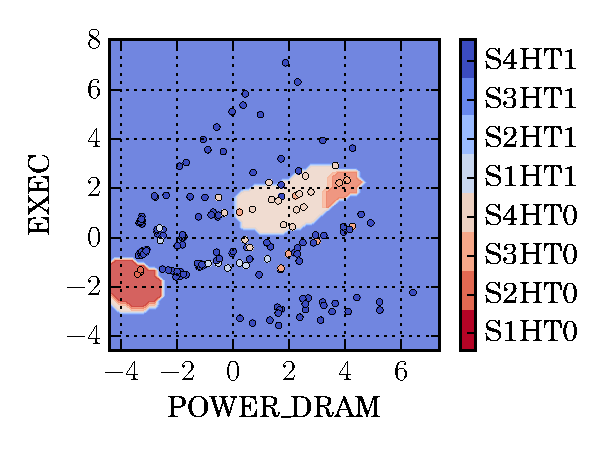
\includegraphics[width=0.3\columnwidth]{figs/classifiers/training_space_svm_ts.pdf}
  \label{fig:feat-svm-ts}
  % \vspace{ -1.5em }
  }
  % \\
  % \vskip -1.5em
  \hspace*{0.1cm}
  \subfloat[DVFS only, recall=0.645.]
  {\centering 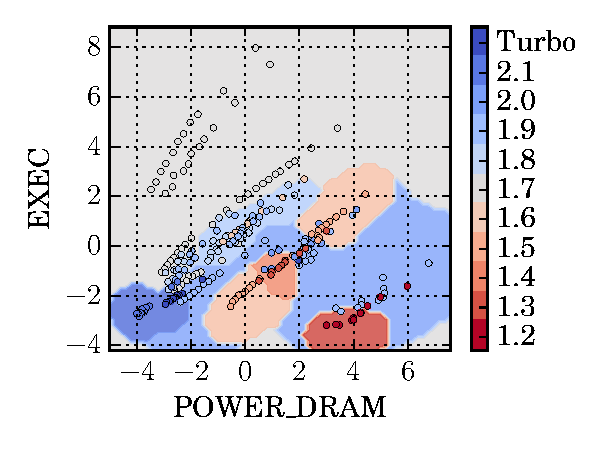
\includegraphics[width=0.3\columnwidth]{figs/classifiers/training_space_svm_dvfs.pdf}
  \label{fig:feat-space-svm-dvfs}
  % \vspace{ -1.5em }
}
\caption{Training data and learned decision boundaries for SVM when classifying for taskset and DVFS separately.}
\label{fig:feat-space-svm-separate}
% \vskip -1.0em
\end{figure}

An alternative approach is for one classifier to predict the taskset, and a separate classifier to predict the DVFS frequency.
\figref{feat-space-svm-separate} visualizes the training and recall for SVM (like \figref{feat-space-svm} in \secref{challenges-learning}) using separate classifiers.
Note that there are fewer data points, as DVFS is fixed at TurboBoost when training for taskset, and taskset is fixed at all sockets and HyperThreads when training for DVFS.
Taskset's recall is quite good, while DVFS is not as good as before.
There is, of course, additional overhead in running two classifiers instead of one, but \secref{classifiers-eval-overhead} demonstrated that data processing overhead is not significant, and there is still only a single instance of PCM and the actuators running.

\begin{figure}[t]
  \centering
  \begin{tikzpicture}
\definecolor{s1}{RGB}{228, 26, 28}
\definecolor{s2}{RGB}{55, 126, 184}
\definecolor{s3}{RGB}{77, 175, 74}
\definecolor{s4}{RGB}{152, 78, 163}
\definecolor{s5}{RGB}{255, 127, 0}

\begin{groupplot}[
    group style={
        group name=plots,
        group size=1 by 1,
        xlabels at=edge bottom,
        xticklabels at=edge bottom,
        vertical sep=5pt
    },
% axis x line* = bottom,
xlabel near ticks,
major x tick style = transparent,
xlabel={},
height=3.5cm,
width=0.95\columnwidth,
xmin=0.5,
xmax=5.5,
enlargelimits=false,
tick align = outside,
tick style={white},
ylabel style={align=center},
ytick=\empty,
ymin=0.6,
ymax=1.1,
ytick={0.6,0.7,0.8,0.9,1.0,1.1},
yticklabels={0.6,0.7,0.8,0.9,1.0,1.1},
legend cell align=left, 
legend style={ column sep=1ex },
ymajorgrids,
grid style={dashed},
]

\nextgroupplot[ylabel={Energy \\ (Normalized)},
ybar=\pgflinewidth,
legend entries = {{Single},{Separate}},
legend style={draw=none,legend columns=5,at={(.5,1.4)},anchor=north},
bar width=8pt,
ylabel shift={0mm},
xticklabel shift={0pt},
x tick label style={rotate=35, anchor=east, font=\scriptsize},
xtick={1,2,3,4,5,6,7},
xticklabels={
{ET},
{GB},
{KNN},
{MLP},
{SVM},
},
execute at end plot={
% "Race":
\draw[thin, dashed] (axis cs:\pgfkeysvalueof{/pgfplots/xmin},1) -- (axis cs:\pgfkeysvalueof{/pgfplots/xmax},1);
% "Best static DVFS":
\draw[thick, dotted] (axis cs:\pgfkeysvalueof{/pgfplots/xmin},0.765646972) -- (axis cs:\pgfkeysvalueof{/pgfplots/xmax},0.765646972);
% "ET_SVM"
\draw[thin, solid] (axis cs:\pgfkeysvalueof{/pgfplots/xmin},0.8288250669) -- (axis cs:\pgfkeysvalueof{/pgfplots/xmax},0.8288250669);
% hack to reset column line style (ghostscript seems to use last formatting as line style, e.g. dashed or dotted instead of solid)
\draw[thin, solid] (axis cs:\pgfkeysvalueof{/pgfplots/xmin},\pgfkeysvalueof{/pgfplots/ymin}) -- (axis cs:\pgfkeysvalueof{/pgfplots/xmax},\pgfkeysvalueof{/pgfplots/ymin});
},
]
\addplot table[x index=0,y index=7, col sep=tab] {img/classifiers/compare_interval/compare_5s.txt};
\addplot table[x index=0,y index=7, col sep=tab] {img/classifiers/compare_pca/sep_clfs.txt};

\end{groupplot}

\end{tikzpicture}
  \caption{Average energy consumption when using a single or separate classifiers for system knobs (lower is better).}
  \label{fig:separate-clfs}
  % \vskip -1.0em
\end{figure}

\figref{separate-clfs} quantifies the behavior when we use two separate classifiers simultaneously.
In each case, the same type of classifier is used for both taskset and DVFS prediction.
In three of five cases, $Separate$ actually outperforms the $Single$ approach.
However, it is also possible for $Separate$ to perform rather poorly, as seen with the MLP classifier.
The average MLP behavior is representative of the applications tested, \ie not caused by an outlier---in three of the four applications evaluated, MLP classifying taskset and DVFS separately performed worse than the \emph{race-to-idle} heuristic.
Of course, taskset and DVFS prediction may benefit from using different classification algorithms.
We tested taskset-only and DVFS-only classifiers in isolation and empirically determined that, for our system and applications, the ET classifier works best for taskset prediction and the SVM classifier works best for DVFS prediction.
The solid horizontal line indicates the energy consumption for this ET/SVM classifier mix.
While this avoided the poor results seen with MLP, it actually performed slightly worse than three of the four remaining $Single$ classifier approaches.
Using a single, unified classifier that learns both taskset and DVFS together ultimately produces more reliable predictions.


\subsection{Discussion of Results and Limitations}
\label{sec:eval-discuss}

Our evaluation demonstrates that machine learning classification driven by low-level features is an effective approach for improving energy efficiency.
In fact, a variety of different classifiers are useful for predicting energy-efficient system settings at runtime, even without classifier tuning.
No single classifier appears to have a clear advantage over others, though future work on fine-tuning the training data and classifiers, combined with evaluations on other platforms, may eventually produce a near-optimal implementation.

We also did not attempt to optimize the runtime's overhead---reading performance counters, data transformations, or system actuation.
Although low, there is still room for improvement, which could support faster sampling and prediction intervals and further improve energy consumption.

We currently only manage socket/core allocation at system-level.
Because applications are launched with a fixed number of threads, those threads are forced to share compute cores when we bind applications to fewer sockets or disable HyperThreads during runtime.
This over-subscription is usually not as efficient as matching the thread count to the available cores, \eg running 80 threads on our 80 physical cores is more efficient that binding 160 threads to those 80 cores.
Integration with application-level parallelism can further improve energy efficiency and reduce resource contention when binding applications to smaller tasksets \cite{Sridharan2013}.
% \TODO{Anything on memory allocation/interleaving? We really don't have a solution to this problem when using dynamic taskset.}

On large systems such as our evaluation platform, the processor and DRAM consume the majority of system power, which we are able to measure \cite{RAPL,PCMGit}.
There are other components like hard disks and network interfaces that are not currently accounted for.
While it is not common practice to instrument these other components for power/energy monitoring, such feedback could help resource management solutions achieve better total energy efficiency.


\chapter{Conclusion}

This dissertation addresses balancing application performance and system energy consumption in computing systems.
The first two projects, POET and CoPPer, are adaptive control-theoretic approaches for meeting soft performance constraints which simultaneously minimize energy consumption.
The third project uses machine learning classification techniques, driven by hardware performance counters, to predict energy-efficient system settings at runtime to optimize the performance/energy tradeoff.
Unlike static resource allocation techniques, our solutions dynamically adjust resource allocations based on runtime feedback to adapt to changing application and system behavior.

Our early work demonstrates that heuristic approaches for meeting timing constraints and reducing energy consumption are not portable between applications and systems, \eg the classic \emph{race-to-idle} heuristic can be completely the wrong approach to use.
Therefore, we propose POET, a portable approach to resource management that functions independent of platform timing/energy tradeoffs or particular system knobs.
POET uses control theory to meet soft performance (or latency) goals and mathematical optimization to minimize energy consumption.
We demonstrate POET's ability to meet soft performance constraints and achieve near-optimal energy consumption on two very different embedded systems---a Vaio tablet with an Intel Haswell processor, and an ODROID-XU+E with a heterogeneous ARM big.LITTLE SoC.
We then demonstrate POET's effectiveness on a dual-socket server-class system with an order of magnitude more knob settings and significantly more compute power than the embedded platforms.
In addition, we briefly discuss Bard, a follow-on project which modifies POET to allow switching between performance or power goals while optimizing energy or performance respectively.
% Furthermore, POET has been used as the foundation for other researchers' projects.

Software management of DVFS is becoming deprecated, necessitating a replacement for the abundance of controllers that previously relied on DVFS to meet performance constraints.
We respond to this demand with CoPPer, which also uses adaptive control-theoretic techniques to meet soft performance goals while optimizing energy.
CoPPer actuates hardware power caps instead of DVFS, but leaves the optimization to the hardware, which can adapt to changing resource demands more quickly than software.
CoPPer addresses new challenges that arise from power capping, without requiring an explicit behavior model.
We evaluate CoPPer on a dual-socket system using Intel RAPL, demonstrate that it meets soft performance constraints, and outperforms a state-of-the-art DVFS controller (a modified version of POET) in achieving low energy consumption.
Additionally, CoPPer introduces a novel \emph{gain limit} to prevent over-allocating power when it is not beneficial, \eg for memory-bound applications or unachievable performance goals.

Finally, we shift focus to the High Performance Computing (HPC) domain and propose optimizing energy efficiency to minimize the runtime cost of computation.
Beyond the obvious cost savings achieved from reducing energy, we extrapolate from our single-system results to show that optimizing energy efficiency in hardware over-provisioned, power-constrained clusters (as we expect future exascale HPC systems to be) increases the total throughput of the cluster to complete more science for the same runtime costs.
To avoid modifying applications, we map low-level hardware performance counters (features) to energy-efficient system knob settings.
We propose using machine learning classification techniques to predict energy-efficient settings in-situ on compute nodes, since they are low-overhead compared to existing estimation approaches used in HPC resource management.
The complexity of the feature space mappings makes simple classification approaches insufficient for solving this resource allocation problem.
We evaluate five of the most promising classifiers and demonstrate that they dramatically reduce the energy consumption of production HPC genome assembly applications on a large shared-memory compute node with low overhead and robustness to the availability of different performance counters.


\section{Future Work}

While this dissertation is on performance and power/energy consumption, there are other tradeoffs available in computing systems.
For example, tuning application accuracy is an ongoing area of research.
A resource allocation scheme could dynamically choose from a set of functions that offer different performance and computation precision, or a configurable hardware component can increase performance or reduce energy consumption at the expense of less accurate results.
Computation accuracy could be a goal or optimization in any of the three major projects presented in this dissertation and would be useful on systems ranging from embedded platforms to HPC clusters.
It is a particularly challenging area of research because different applications have different concepts of what it means to be accurate.
Accuracy can also be difficult to quantify, especially when such values are dependent on human perception, \eg for various types of multimedia.
Furthermore, the range of acceptable accuracies is context-dependent, \eg by application and/or deployment scenario.

Our control-theoretic projects support meeting a single constraint and optimizing in another dimension.
However, software must often manage multiple constraints, \eg meet a performance goal but also respect a power cap.
Combining multiple controllers is a logical next step, but they must be coordinated so as not to conflict with each other.
In simple cases, controllers tune knobs that do not affect each other, in which case little or no direct coordination is needed, \eg one controller tunes application-level knobs while another tunes system knobs.
Otherwise the controllers must either communicate directly or be configured such that they can still adapt correctly, \eg by using different pole values and/or window periods.
In either case, they should not be tuning the same knobs, otherwise their internal state would be inaccurate---they would fail to meet their constraints and any optimization they attempt to provide could suffer as well.

Our machine learning classification framework currently optimizes energy efficiency on individual compute nodes for single-node jobs.
To actually maximize the throughput of hardware over-provisioned, power-constrained clusters, the solution must be adapted to scale out to multiple nodes.
Naively deploying the current solution on all nodes in a cluster will not achieve this, and could result in less-than-optimal energy efficiency and violations of the global power constraint.
First, a component to schedule jobs while respecting the cluster power constraint is needed, likely in coordination with accurate predictions of how much power individual nodes require while running their assigned jobs energy-efficiently (keeping in mind that the power consumption fluctuates as applications move through phases).
Additionally, tighter coordination between nodes is needed to support jobs that scale across multiple nodes, so that one node does not slow down the rest, resulting in reduced total energy efficiency.
A scaled-out approach will need to account for other components like network switches and consider the location of different compute nodes---individual racks have their own power constraints, and the distance between communicating nodes impacts application performance.
% Our machine learning classification framework optimizes energy efficiency, but can be easily adapted to support different goals derived from performance counters.

System resources other than CPU and DRAM should be coordinated since they also impact performance/power tradeoffs---GPUs and other accelerators are particularly interesting.
Data storage (\eg hard disks, SSDs, future non-volatile memories) and network interfaces are also critical, particularly in low-power environments like embedded systems and high-throughput and communication-intensive environments like HPC.

Unfortunately, power/energy sensors on modern computing systems are relatively rare, with the exception of Intel processors.
Model-based approaches are too inaccurate and cannot provide runtime guarantees, and custom/ad-hoc instrumentation requires special equipment and does not scale well in production.
To better enable energy-aware applications, more hardware needs to include power/energy instrumentation---not just on processors and SoCs, but on other hardware components as well, \eg DRAM, disks, and networking components.
Such capabilities would more easily enable both research and development of practical solutions for coordinating a wide variety of system resources in an energy-aware manner.
Similarly, datacenters and HPC clusters can benefit from instrumenting external components like network switches and network-attached storage devices.

Finally, the availability of runtime feedback from which to make informed decisions is a fundamental requirement of self-aware systems.
Applications and users want to specify contextual goals, \eg frames processed in a video encoder, not low-level metrics like instructions retired.
Hardware performance counters are the de facto standard today, but do not provide high-level metrics like a true measure of application progress.
Few such mechanisms are currently available, and typically require modifying applications to provide appropriate instrumentation, \eg using Heartbeats.
Language constructs or operating system interfaces could provide more portable approaches for applications to report metrics.
Some measurements could potentially be inferred from the software design, or at least only require a developer to specify a few attributes in their code without linking to additional libraries.
A self-aware system can then rely on these portable metrics rather than requiring the developer to provide instrumentation.


\appendix
\chapter{Tools for Self-aware Systems Research}
\label{app:tools}

Tool building is often under-appreciated by the computer science research community, yet is crucial to enabling practical systems research.
The projects in this dissertation led to the development of a variety of portable tools that we make available to the community at large.
Links to published code are available in \appref{urls}.

In \secref{intro-description}, we described the \emph{observe}, \emph{decide}, and \emph{act} framework that Hoffmann proposed in his ``self-aware'' computing model \cite{HoffmannPhD}.
While the core research in this dissertation focuses on the \emph{decide} phase, the tools described in this chapter are relevant to the \emph{observe} and \emph{act} phases.


\section{Runtime Instrumentation and Profiling}
\label{app:profiling}

The control-theory based projects presented in this dissertation (POET, Bard, CoPPer) are designed for applications that have high-level loops for which we enforce predictable timing behavior.
For applications to capture performance and power/energy data, they need a mechanism to capture and record metrics.
Application developers often create their own instrumentation and profiling tools, which is mostly unnecessary and means that data is stored in a variety different formats, making it troublesome to process.
Hoffmann \etal proposed \interface{Heartbeats} to specify and record performance goals for self-aware applications \cite{icac2010heartbeats}.
We extended this work in POET and Bard and released \interface{Heartbeats 2.0}, which includes a primitive interface for portably capturing energy metrics.

We later developed a simplified interface, aptly called \interface{Simple Heartbeats}, which allows more flexibility in recording application behavior.
For example, it can record performance and power behavior for discontinuous loops or separate application code phases and is more portable across operating systems.
Java and Rust language bindings and abstractions are also available for Simple Heartbeats, some of which are integrated with Servo, Mozilla's parallel web browsing engine \cite{servo}.
These code bases are also used in other projects not described in this dissertation.

We also created \interface{Heartbeats Simple Classic} which wraps Simple Heartbeats and EnergyMon (described in the next section) while behaving more like Heartbeats 2.0.
This interface benefits from the simplicity of the original Heartbeats design while maintaining portability, and is used in CoPPer's evaluation.


\section{EnergyMon: A Portable Interface for Runtime Energy Monitoring}
\label{app:energymon}

There is a growing need for software to access power and energy data in-situ, like for the projects in this dissertation.
Designing and evaluating POET and Bard led us to conclude that a portable software interface for accessing energy metrics at runtime is necessary.
The primitive interface in Heartbeats 2.0 is not as portable as needed and does not allow capturing power/energy data in isolation.
In response, we designed \interface{EnergyMon}.

Accessing power/energy data requires writing system-specific code which is challenging for researchers and engineers, and results in applications that are not portable across platforms.
The diversity in sensor properties and current ad-hoc approaches for using them presents a significant challenge.
The problem is more complex than simply locating and reading the correct files, hardware registers, or memory addresses.
A portable interface must account for other factors:
\begin{itemize}
\item \textbf{Data Type:} Whether sensors expose \emph{power} or \emph{energy} data.
\item \textbf{Access:} Privileges/constraints, \eg \emph{exclusive access}, particularly for external devices.
\item \textbf{Units of measurement:} The power or energy units that sensors expose measurements in, and also their \emph{level of precision}.
\item \textbf{Overflow:} Maximum values for sensor counters.
\item \textbf{Refresh Interval:} How frequently sensors update.
\item \textbf{Interface:} System abstractions, protocols, and data formats.
\end{itemize}
Sensors which only report power data \emph{must be polled} at their refresh interval so as not to lose data after the sensor refreshes.
Power/energy readings may need to be \emph{extracted from other data} or \emph{transformed} before they are meaningful~\cite{WattsUp,OSP,SandyBridge}.
Developers may even have to implement different \emph{protocols} and \emph{data formats}~\cite{WattsUp,OSP}.
Furthermore, even a single system equipped with power or energy monitoring can offer multiple approaches to obtain it~\cite{RAPL,ina231,SandyBridge}.
Correctly and accurately collecting power and energy data requires understanding and properly managing sensor properties and behavior.

The first important design decision is which \emph{data type} to expose in a common interface.
We choose energy, which unlike power, is not explicitly a function of time and can be recorded cumulatively, simplifying the interface.
With an energy provider that records total energy consumed since some time $\tau = 0$, a power-aware application can simply record energy $E$ at the beginning and end of a time interval and compute the average power as $\Delta E / \Delta \tau$.
In this way, the interface easily supports applications interested in energy or power.

Next, a common interface can expose energy metrics in a standard and sufficiently precise \emph{unit of measurement} at a large enough data length to avoid \emph{overflow}.
Applications therefore do not need to track various unit types and do conversions.
A deceptively simple but important insight is not our choice of units or data length, but rather that counter overflow is one of the diverse sensor properties that applications should not have to worry about.
We choose microjoules as 64-bit unsigned integers which are precise enough for the use cases we anticipate and avoid the need for floating point data types.
At $100$ W of power, it would take about 5,850 years to overflow, and in our experience, modern sensors are too imprecise and models too inaccurate to justify smaller units.

The \interface{EnergyMon} C interface defines an \struct{energymon} struct that contains seven function pointers and a \variable{state} variable:
\begin{itemize}
\item \variable{finit}: Initialize the energy monitor.
\item \variable{fread}: Get the cumulative energy in microjoules.
\item \variable{ffinish}: Destroy the energy monitor.
\item \variable{fsource}: Get the name for the energy monitoring source.
\item \variable{finterval}: Get the refresh interval in microseconds.
\item \variable{fprecision}: Get the best possible precision in microjoules.
\item \variable{fexclusive}: Get if exclusive access is required.
\item \variable{state}: Pointer to a struct that the implementation uses to maintain internal state, \eg file descriptors or thread data.
\end{itemize}
This interface exposes some of the diverse properties described previously, like \emph{refresh interval} and sensor \emph{precision}, while hiding other properties that are not important to most software, like the \emph{underlying interfaces}, \emph{device protocols}, and \emph{data formats}.

For any time $\tau$, where $\tau=0$ is the energy monitor's initialization, the following invariants hold for energy readings $E(\tau)$:
\begin{eqnarray}
  \forall \tau \ge 0 && \tau_i \le \tau_j \implies 0 \le E(\tau_i) \le E(\tau_j) \label{eqn:energy-monotonic} \\
  && \tau = 0 \not \implies E(\tau) = 0 \label{eqn:energy-time-zero}
\end{eqnarray}
\eqnref{energy-monotonic} states that for any time at or after initialization, energy is always non-negative and monotonically increasing.
\eqnref{energy-time-zero} states that the initial value does not have to be zero (could be larger).
The following example of the EnergyMon C interface demonstrates computing the average power of a worker function (error checking excluded):
\lstset{emph={%  
    energymon, energymon_get_default, finit, fread, ffinish%
    },emphstyle={\color{black}\bfseries\underbar}%
}%
\begin{lstlisting}[language=C,%
  caption={Reading energy values and computing power with EnergyMon.},%
  morekeywords={uint64_t},%
  label={lst:energymon-example}]%

energymon em;
uint64_t start_uj, end_uj, start_usec, end_usec;

// get the energymon instance and initialize
energymon_get_default(&em);
em.finit(&em);

// get start time/energy
start_usec = gettime_us(); // e.g. wrap clock_gettime
start_uj = em.fread(&em);

// application-specific processing
do_work();

// get end time/energy
end_usec = gettime_us();
end_uj = em.fread(&em);

printf("Average power of do_work() in Watts: %f\n",
       (end_uj-start_uj) / (double) (end_usec-start_usec));

// destroy the instance
em.ffinish(&em);
\end{lstlisting}
Other functions provide additional information about the implementation that software can use to make runtime decisions.
For example, applications can use the name provided by \variable{fsource} for debugging or logging.
\variable{finterval} can be used to determine a lower bound on sleep time for polling the energy monitor at regular intervals.
\variable{fprecision} might inform a self-adaptive system how much noise to expect in power/energy data.
\variable{fexclusive} could be used in deciding to share energy data with other software components.
The project also includes command-line utilities for integration with shell scripts, although we do not describe them further here.

EnergyMon was integrated with Servo, Mozilla's parallel web browsing engine \cite{servo}.
A complete design and evaluation is available in the original publication \cite{energymon} and an extended technical report \cite{EnergyMonTR}.
EnergyMon is also used in CoPPer's evaluation, as well other research projects not described in this dissertation, \eg the ongoing development of the FAST language described in \secref{intro-ee}.


\section{Power Capping}
\label{app:powercap}

Evaluating Intel RAPL \cite{RAPL} ultimately led to the design and evaluation of the CoPPer project.
Again, we found a distinct lack of tools to aid us---most material we found used low-level approaches for interfacing with RAPL that were hardware-dependent and required detailed understanding of RAPL as defined in Intel's software developer's manuals \cite{intel-sdm}.

In recent years, the Linux kernel exposed some RAPL functionality via the \interface{powercap} file system interface \cite{powercap}.
Perhaps the biggest advantage of the powercap interface is that a user does not have to configure the system's model-specific registers, which have very particular platform-dependent encodings.
However, there were no software utilities available to assist in discovery of these RAPL capabilities, or in proper system actuation.
We therefore developed a \interface{Linux powercap bindings} library and collection of applications to aid software developers with these tasks.
These tools are now available in repositories for Debian-based Linux distributions, including Ubuntu 18.04 LTS ``Bionic Beaver'' and newer.
The library usage is straightforward, for example (error checking excluded):
\lstset{emph={%  
    powercap_rapl_pkg, powercap_rapl_get_num_packages, powercap_rapl_init, powercap_rapl_set_power_limit_uw, powercap_rapl_destroy%
    },emphstyle={\color{black}\bfseries\underbar}%
}%
\begin{lstlisting}[language=C,%
  caption={Setting RAPL power caps with the powercap library.},%
  morekeywords={uint32_t},%
  label={lst:powercap-example}]%

uint32_t i, npackages;
powercap_rapl_pkg* pkgs;

// get number of processor sockets
npackages = powercap_rapl_get_num_packages();

// initialize
pkgs = malloc(npackages * sizeof(powercap_rapl_pkg));
for (i = 0; i < npackages; i++) {
  // last parameter is a "read-only" flag (set to false)
  powercap_rapl_init(i, &pkgs[i], 0);
}

// set caps of 100 Watts for short_term, 50 Watts for long_term constraints on each package
for (i = 0; i < npackages; i++) {
  powercap_rapl_set_power_limit_uw(&pkgs[i], POWERCAP_RAPL_ZONE_PACKAGE, POWERCAP_RAPL_CONSTRAINT_SHORT, 100 * 1000000);
  powercap_rapl_set_power_limit_uw(&pkgs[i], POWERCAP_RAPL_ZONE_PACKAGE, POWERCAP_RAPL_CONSTRAINT_LONG, 50 * 1000000);
}

// now cleanup
for (i = 0; i < npackages; i++) {
  powercap_rapl_destroy(&pkgs[i]); {
}
free(pkgs);
\end{lstlisting}
Command-line utilities, not described further here, also make integration with scripts easy.

While the powercap interface is sufficient for many use cases, it has some limitations.
First, the configuration is not as fine-grained as it could be due to the kernel developers' choice of data units (microjoules, microwatts, and microseconds).
Second, it is only useful on systems running the Linux kernel.
We address these limitations with \interface{RAPLCap}, a more general interface for accessing RAPL that provides multiple implementations.
The two primary implementations are for Linux---the first wraps the Linux powercap bindings library; the second accesses the system model-specific registers which allows more fine-grained configuration, but must be updated as new hardware becomes available.
The RAPLCap interface is also straightforward to use, for example (error checking excluded):
\lstset{emph={%  
    raplcap, raplcap_limit, powercap_rapl_init, raplcap_destroy, raplcap_set_limits%
    },emphstyle={\color{black}\bfseries\underbar}%
}%
\begin{lstlisting}[language=C,%
  caption={Setting RAPL power caps with RAPLCap.},%
  morekeywords={uint32_t},%
  label={lst:raplcap-example}]%

raplcap rc;
raplcap_limit rl_short, rl_long;
uint32_t i, nsockets;

// get the number of RAPL packages/sockets
nsockets = raplcap_get_num_sockets(NULL);

// initialize
raplcap_init(&rc);

// set caps of 100 Watts for short_term, 50 Watts for long_term constraints on each socket
// a time window of 0 leaves the time window unchanged
rl_short.watts = 100.0;
rl_short.seconds = 0.0;
rl_long.watts = 50.0;
rl_long.seconds = 0.0;
for (i = 0; i < nsockets; i++) {
  raplcap_set_limits(&rc, i, RAPLCAP_ZONE_PACKAGE, &rl_long, &rl_short);
}

// cleanup
raplcap_destroy(&rc);
\end{lstlisting}

Using a common interface allows software to link against different library implementations, depending on the target hardware platform or operating system, without requiring changes to application code.
Work is ongoing to implement RAPLCap on other operating systems like Apple OSX and Microsoft Windows, which expose different methods for configuring RAPL.
RAPLCap also includes command-line utilities, which are not described further here.

\chapter{Published Code}
\label{app:urls}

This appendix provides links for much of the source code developed as part of this dissertation.
Note that locations may change with time, and APIs may change from their presentation in this dissertation as demands evolve.
Projects generally contain usage instructions and citation information.
In general, bug reports and code patches (\eg pull requests) are welcome.

\tblref{project-code} provides URLs for the core research code in this dissertation.

\begin{table}[ht]
\scriptsize
\centering
\caption{Project code URLs.}
\begin{tabular}{lcr}
  \textbf{Project} & \textbf{Language} & \textbf{URL} \\
  \hline
  \hline
  POET/Bard Resources & -- & http://poet.cs.uchicago.edu \\
  POET & C & https://github.com/libpoet/poet \\
  Bard & C & https://github.com/libpoet/bard \\
  \hline
  CoPPer & C & https://github.com/powercap/copper \\
  CoPPer Evaluation Helper \& Resources & C & https://github.com/powercap/copper-eval \\
  \hline
  \hline
\end{tabular}
\label{tbl:project-code}
\end{table}

\tblref{tool-code} provides URLs for code developed to assist the research in this dissertation that may be useful for wider audiences.

\begin{table}[ht]
\scriptsize
\centering
\caption{Tool code URLs.}
\begin{tabular}{lcr}
  \textbf{Tool} & \textbf{Language} & \textbf{URL} \\
  \hline
  \hline
  Heartbeats 2.0 & C & https://github.com/libheartbeats/heartbeats \\
  Simple Heartbeats & C & https://github.com/libheartbeats/heartbeats-simple \\
  Simple Heartbeats Classic & C & https://github.com/libheartbeats/heartbeats-simple-classic \\
  Simple Heartbeats Rust Bindings & Rust & https://github.com/libheartbeats/heartbeats-simple-sys \\
  Simple Heartbeats Rust Abstractions & Rust & https://github.com/libheartbeats/heartbeats-simple-rust \\
  Simple Heartbeats Java Bindings/Abstractions & Java & https://github.com/libheartbeats/heartbeats-simple-jni \\
  \hline
  EnergyMon & C & https://github.com/energymon/energymon \\
  EnergyMon Rust Bindings & Rust & https://github.com/energymon/energymon-sys \\
  EnergyMon Rust Abstractions & Rust & https://github.com/energymon/energymon-rust \\
  EnergyMonitor Rust Trait & Rust & https://github.com/energymon/energy-monitor-rs \\
  EnergyMon Java Bindings/Abstractions & Java & https://github.com/energymon/energymon-jni \\
  \hline
  Linux powercap bindings & C & https://github.com/powercap/powercap \\
  RAPLCap & C & https://github.com/powercap/raplcap \\
  \hline
  \hline
\end{tabular}
\label{tbl:tool-code}
\end{table}


% Format a LaTeX bibliography
\printbibliography
%\makebibliography

\end{document}
